The main challenge, in this analysis, is to achieve reliable predictions of the low Standard Model background 
leading to the same-sign leptons + jets final state. 
This background is composed partly of rare processes such as the associate production of a top quark pair with a massive boson, 
or the production of multiple bosons. 
The other contribution consists in experimental backgrounds originating from the imperfect discrimination between prompt leptons and other objects, 
or the occasional misreconstruction of the electron charge. 
The following sections provide more details about the nature of these different categories of background, 
and the foreseen methods that will be used to estimate their contributions to the signal regions. 

%%%%%%%%%%%%%%%%%%%%%%%%%%%%%
\subsection{Backgrounds with prompt SS dilepton or three leptons}
\label{sec:bkg_prompt}

There are two main sources of Standard Model background leading to pairs of same-sign prompt leptons: 
\begin{itemize}
\item[$\bullet$] The associate production of top quark(s) and massive bosons, where the same-sign leptons pair 
originates from leptonic decays of one of the top quarks and of the boson. 
These processes are characterized by a large jet multiplicity, the presence of $b$-jet(s), 
and always have intrinsic missing momentum. 
Therefore they generally represent the largest contribution to the signal regions. 
The dominant processes are $pp\to t\bar{t}W(j)$, $pp\to t\bar{t}Z(j)$ and $pp\to t\bar{t}H$, 
while there are also minor contributions from $pp\to tZbj,\,t\bar{t}WW$, and $pp\to t\bar{t}t\bar{t}$. 
\item[$\bullet$] The production of multiple massive bosons. 
These processes have generally low jet multiplicities. 
However, due to their larger cross-sections, they contribute in a significant way to the background entering signal regions without $b$-jets requirements. 
The dominant processes include $pp\to W^\pm W^\pm jj,\,WZ,\,ZZ$, 
with minor contributions from $pp\to\,WH,\,ZH,\,VVV$ and $H\to\,ZZ\to\,\ell\ell\ell\ell$ or $H\to\,WW\to\,\ell\nu +X$. 
\end{itemize}

We estimate the contributions of these various processes to the signal regions by relying on the Monte-Carlo predictions, 
normalized with the best known theoretical cross-sections: these processes are too rare to allow use of control regions until a significant integrated luminosity will be collected. 
For example, in~\cite{Ducu:2021084} which establishes projections of the sensitivity 
to the $ttH$ signal strength in a final state very similar to this analysis, 
the impact of adding control regions for $t\bar t+V$ processes was found to be favorable only after collecting $\sim 100$~\ifb~of data. 

Processes containing top quarks ($\ttbar + X$) have cross-sections below 1~pb, which have consequently not yet been much constrained experimentally. On the theoretical side, uncertainties on the cross sections are typically large: 30\% for $t\bar{t}W$ and 50\% for $t\bar{t}Z$ for the same-sign $\sqrt{s}=7$~TeV analysis~\cite{NoteSS3L_7TeV}, 22\% for both $t\bar{t}W$ and $t\bar{t}Z$ for the $\sqrt{s}=8$~TeV analysis~\cite{noteSS3L}. 

Cross-sections for diboson processes are known with a rather good accuracy, but only for the inclusive processes, 
while we are mostly interested in processes where several additional partons are produced, 
which carry subsequent additional uncertainties. 

The validation regions described in section~\ref{sec:bkg_VR} help us to ensure that our understanding of these processes is sufficiently reliable, and that the systematic uncertainties assigned to the estimated rates are reasonable. 

%%%%%%%%%%%%%%%%%%
%
\subsection{Charge flip leptons}
\label{sec:bkg_chflips}

The lepton charge mis-measurement commonly referred to as ``charge flip'' background, 
is an experimental background strongly associated to analyses relying on same-sign leptons final states. 
In those events, the electric charge of one of the two leptons forming an opposite-sign (OS) pair, coming from an abundant SM process ($pp\to Z,\,t\bar{t},\,W^+W^-$\ldots), is mis-identified leading to a much rarer SS pair event. 
The most frequent origin of this mis-identification is the following: 
when an electron goes through a medium (in this case, the ATLAS inner detector), it can produce a hard photon by Bremsstrahlung radiation which can then convert in an $e^+e^-$ pair. If the converted electron with the largest $\pt$ has an opposite charge compared to the original electron (the one that emits the hard photon), wrong sign will be assigned to the initial electron track, leading to a charge-flip event. Errors on the track charge assignment itself may occur as well, but they are much rarer. 

We rely on a purely data-driven method to estimate yields of events with charge flipped electrons. 
Assuming one knows the electron charge flip rates $\xi(\eta,p_T)$, a simple way to predict these yields is to select 
events with pairs of opposite-sign leptons in data and assign them a weight: 

\begin{align}
w = \xi\left(\eta^{1},p_T^{1}\right)\left[1-\xi\left(\eta^{2},p_T^{2}\right)\right] 
+ \xi\left(\eta^{2},p_T^{2}\right)\left[1-\xi\left(\eta^{1},p_T^{1}\right)\right] 
\end{align}
where $\xi=0$ for muons. 

The advantages of this method are a good statistical precision since the charge flip rate is quite small, 
and the lack of dependency on the simulation and related uncertainties. 
Obviously, it requires a precise measurement of the rates, which is described in the next paragraph. 
A slight inconvenient is that the reconstructed electron energy, for charge flipped electrons, 
tends to be negatively biased (too low by a few~\GeV), because of the hard Bremsstrahlung at the origin of the charge flip. 
Simply reweighting electrons from opposite-sign lepton pairs therefore does not predict correctly the charge-flip background shape 
for variables strongly dependending on the electron momentum. 
But we do not rely on such discriminant variables, therefore we simply neglect this effect for the moment. 

In order to correctly define this background and to estimate the number of charge flip events in our signal regions, one has to measure the rate (probability) of electron charge mis-measurement. The probability of mis-identifying a muon was found to be negligible, at least for the $\pt$ range considered in this analysis. 
This section is organized as follows: first the procedure to extract the charge flip rate is explained and then, 
the charge flip rates measured with the 2015 dataset are presented. 
A dedicated study of the charge flip rates in different MC productions (MC12, DC14, MC15) can be found in Appendix~\ref{app:flips}.


\par{\bf Measurement of the charge flip rates}

The charge flip rate is extracted with a data-driven technique using a likelihood fit, within a $Z$ boson control sample defined by requiring a pair of SS or OS electrons with invariant mass between 75 and 100 GeV. Since the amount of material the electrons pass through is related to $\eta$, the probability of mis-measuring the charge will depend on $\eta$. Moreover, since the inner detector track curvature is used to measured the charge, the charge flip rate will also be dependent on the electron $\pt$.  
The extraction of charge flip rates will then be performed for a specific ($\eta, \pt$) binning in order to take into account those effects. In the following, the total number of bins is defined as the product of number of $\eta$ bins and number of $\pt$ bins: \# (total bins) = \# ($\eta$ bins) $\times$ \# ($\pt$ bins). The notation "bin $A$", where $A$ can take any values between 0 and \# (total bins), refer to one specific combination of ($\eta,\pt$) bins.

The likelihood fit used to measure the charge flip rate maximizes the function

\begin{equation}
\label{eq:llh}
L = \prod_{I, J} L_{\epsilon(I),\epsilon(J)},
\end{equation}

where $L_{\epsilon(I),\epsilon(J)}$ is the following Poisson distribution:

\begin{equation}
\label{eq:pois}
L_{\epsilon(I),\epsilon(J)} = P(N_{SS}^{obs} | \epsilon(I), \epsilon(J)) = \frac{(N_{SS}^{exp})^{N_{SS}^{obs}} e^{-N_{SS}^{exp}} } {N_{SS}^{obs} !}.
\end{equation}

At this point, we set that the leading electron coming from $Z$ boson falls into bin $I$ while the subleading electron falls into bin $J$. In eq. \ref{eq:llh} and \ref{eq:pois}, $\epsilon(I)$ ($\epsilon(J)$) is then the probability of mis-measuring the charge of an electron that falls into bin $I$ ($J$). The variable $N_{SS}^{obs}$ stands for the observed number of SS events while $N_{SS}^{exp}$ is the expected number of SS events and is defined as:

\begin{equation}
\label{eq:nss}
N_{SS}^{exp} = N ( (1-\epsilon(I))\epsilon(J) + (1-\epsilon(J))\epsilon(I) ),
\end{equation}

with $N$ the total number of events. 
This likelihood fit method is performed with a {\tt TMinuit} routine 
and returns a charge flip rate values for each different ($\eta,\pt$) bin 
as well as the associate statistical errors.

\par{\bf Charge flip rate results}

The comparison of charge flip rates extracted from Monte Carlo simulation and data is important in order to validate our choice of control region. 
In this section, the first results of charge flip rates measured in data are compared to the rates from an MC15 $Z\to e^+e^-$ sample.
To extract the \textit{nominal} charge flip rates, both electrons forming the SS or OS pair must pass the signal selections. 
As explained further in section~\ref{sec:bkg_matrix_method}, the method used to predict the yields of fake leptons requires estimates of the charge flip background 
also for baseline electrons failing the signal requirements. 
A similar methodology is used to extract the charge flip rates for pre-selected (non-signal) electrons 
albeit modified according to the specificities of the measurement (larger background, asymmetry between the definitions of the two selected electrons). 
For this last measurement, the definition of the binning in eq. \ref{eq:llh} to \ref{eq:nss} is different. Instead of referring to the leading and sub-leading electron, $I$ will refer to the bin where the signal electron falls, while $J$ refer to the bin where the non-signal electron falls. Then, $\epsilon(I)$ ($\epsilon (J)$) becomes the probability of mis-measuring the charge of a signal (non-signal) electron that falls into bin $I$ ($J$). In other words, there is no requirement for the leading electron to be neither the signal nor the non-signal electron of the pair.

Figure~\ref{fig:ptsig} shows kinematic $\pt$ distributions, before the background subtraction, 
for nominal measurement on left and loose measurement on right while the $\eta$ distributions are shown on Figure~\ref{fig:etasig}. 
In those plots, the electrons forming an OS (black filled dots for data, blue area for MC) and a SS pair (black circle for data, green area for MC) 
are shown separately and the MC areas are normalized (scaled) to the data luminosity.
% For both Figure~\ref{fig:ptsig} and~\ref{fig:etasig}, the agreement between data and MC is good. 
% -> commented out because it's not tru for loose electrons, because of the background (no mll cut applied in the figure -> large bkg...)
The small discrepancies at low $\pt$ may be due to some Drell-Yan processes that are not considered here 
and to the presence of fake electrons in the loose distributions. The discrepancies in the central region for the loose SS distribution on the right plot of Figure \ref{fig:etasig} can also be attributed to the presence of fake electrons in the sample. 


%------------------------------------------------
\begin{figure}[!htb]
\centering
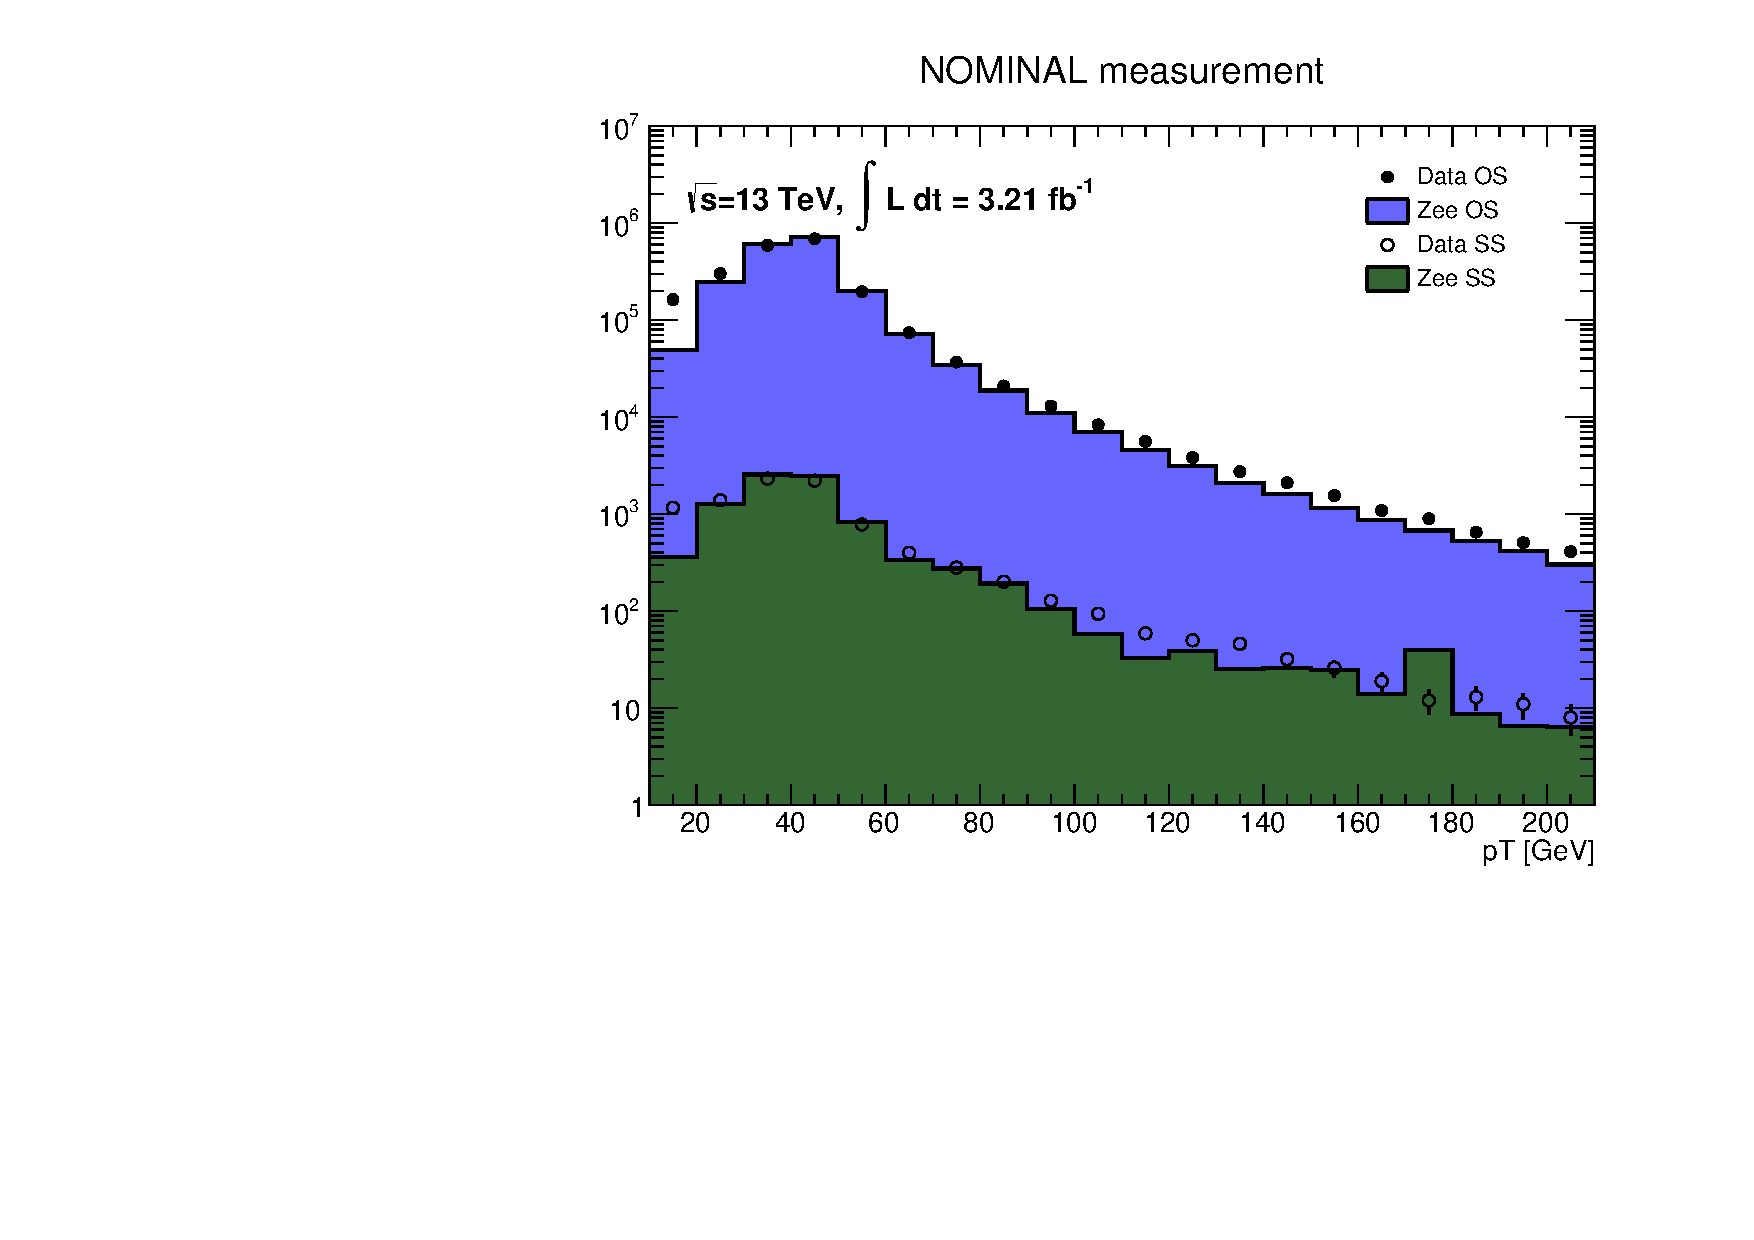
\includegraphics[width=0.4\textwidth]{FIGURES/BKG/chargeFlip/pt_nominal_v28.pdf}
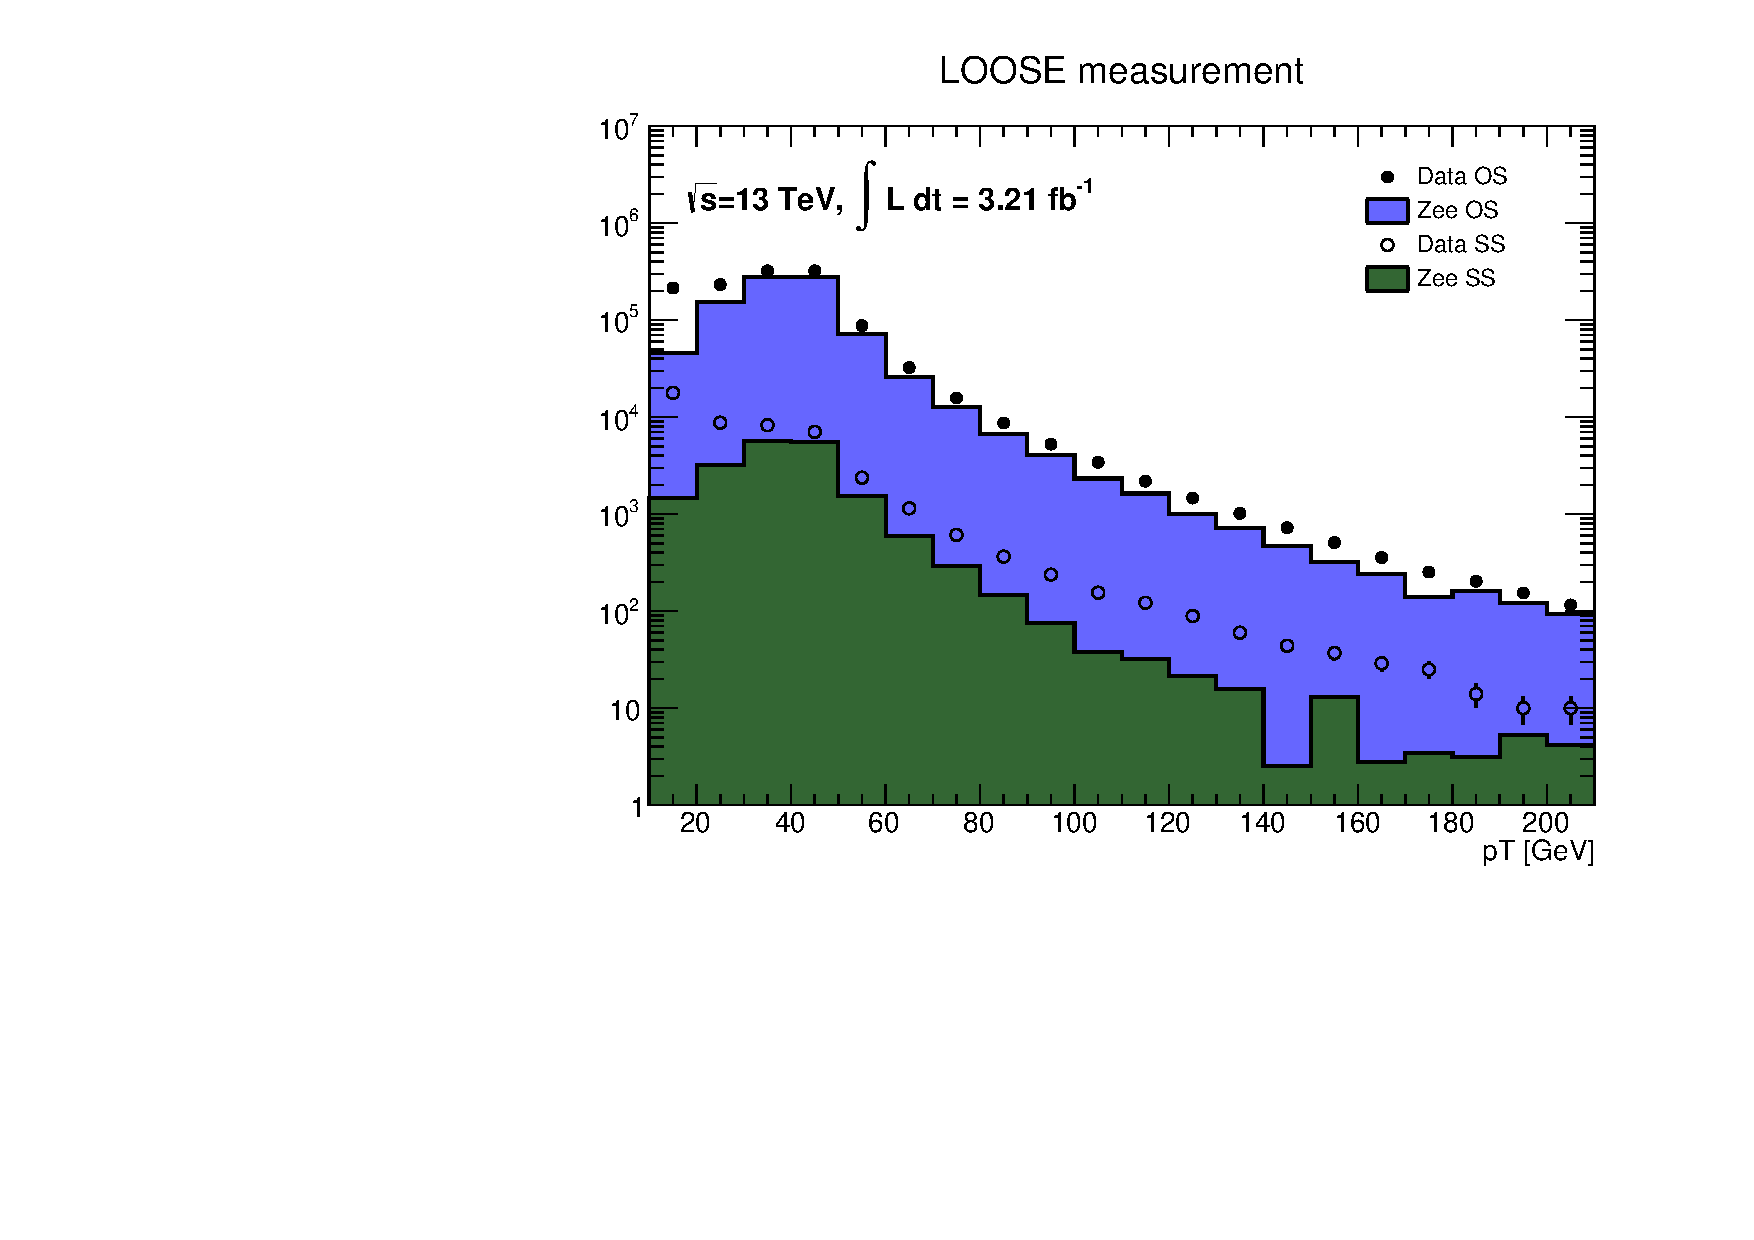
\includegraphics[width=0.4\textwidth]{FIGURES/BKG/chargeFlip/pt_loose_v28.pdf}
\caption{\label{fig:ptsig} $\pt$ distributions for nominal (left) and loose (right) measurements for signal electrons forming an OS pair (filled dots for data, blue area for MC) and a SS pair (empty circles for data, green area for MC). Only statistical uncertainties are shown.}
\end{figure}
%------------------------------------------------

%------------------------------------------------
\begin{figure}[!htb]
\centering
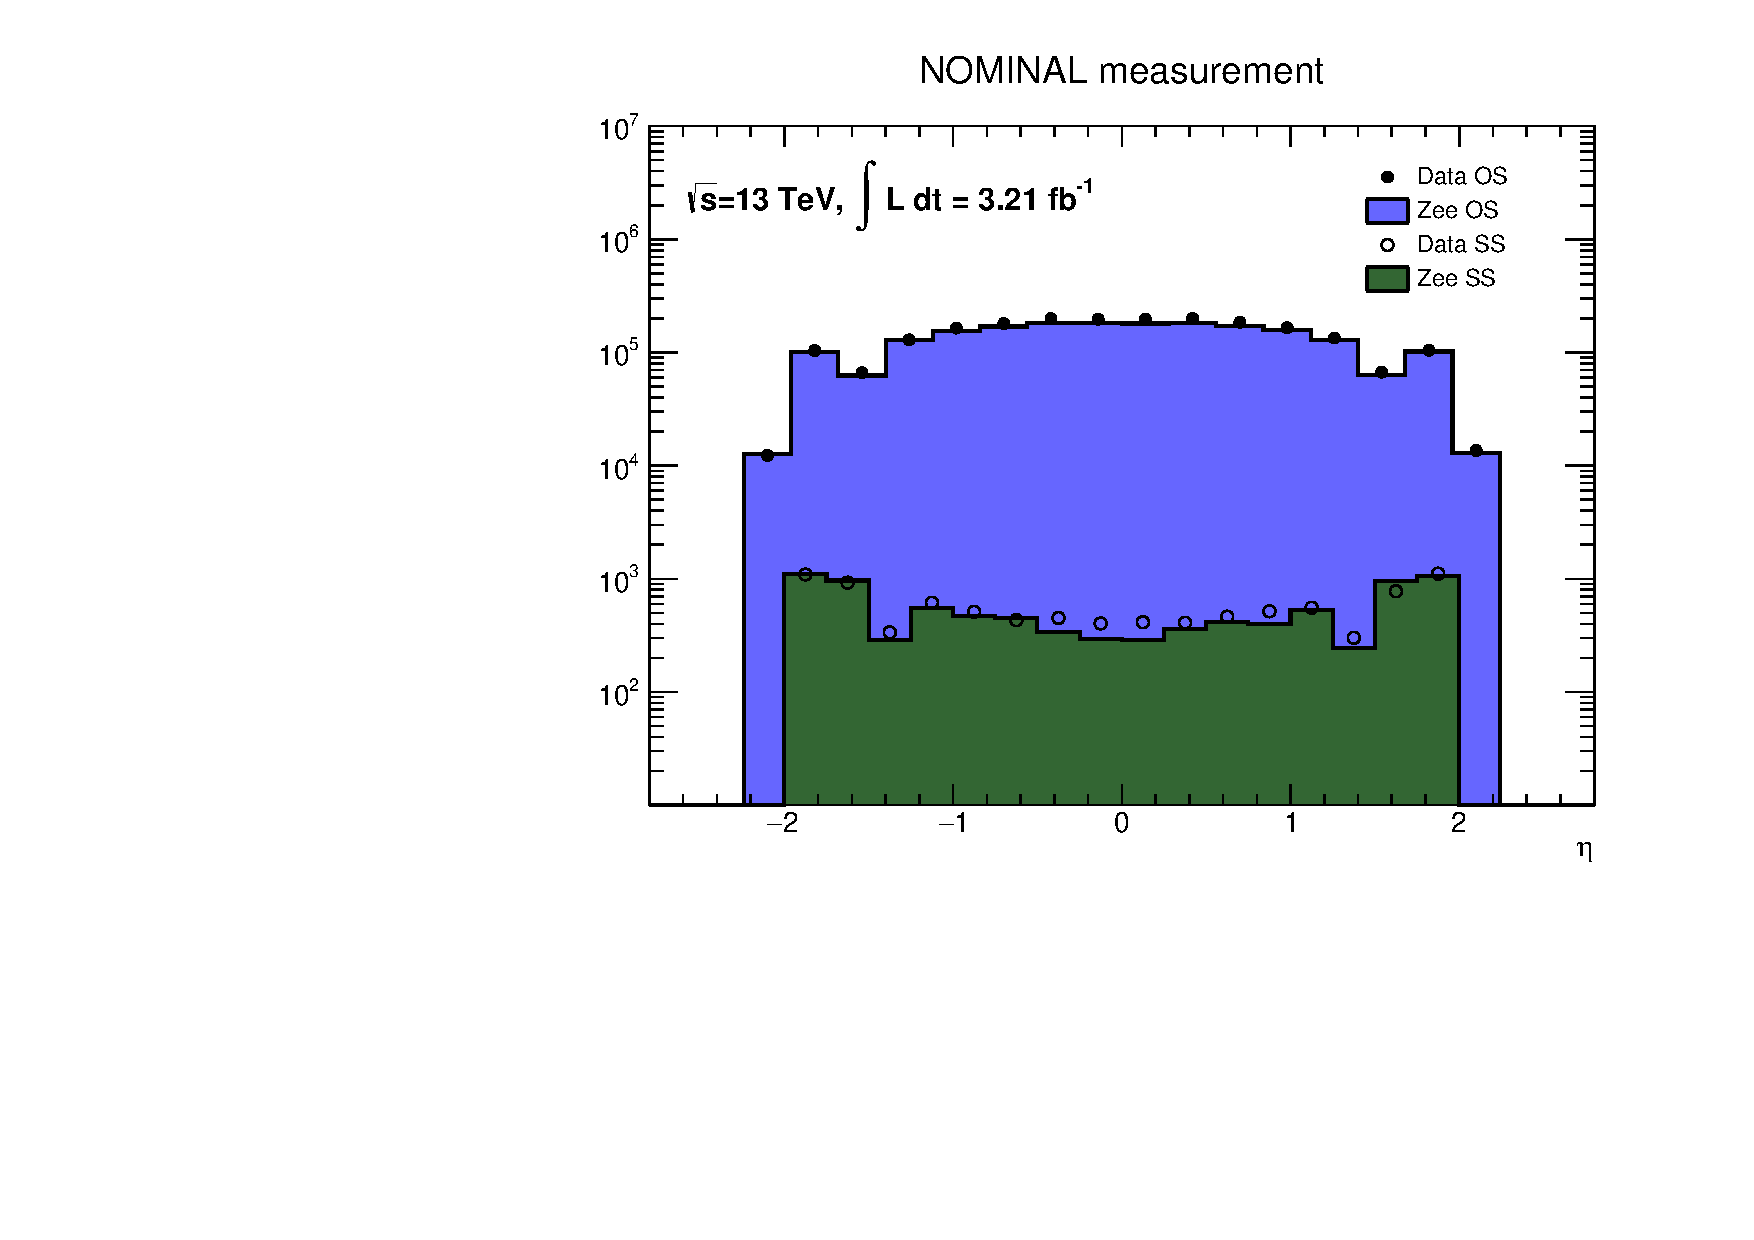
\includegraphics[width=0.4\textwidth]{FIGURES/BKG/chargeFlip/eta_nominal_v28.pdf}
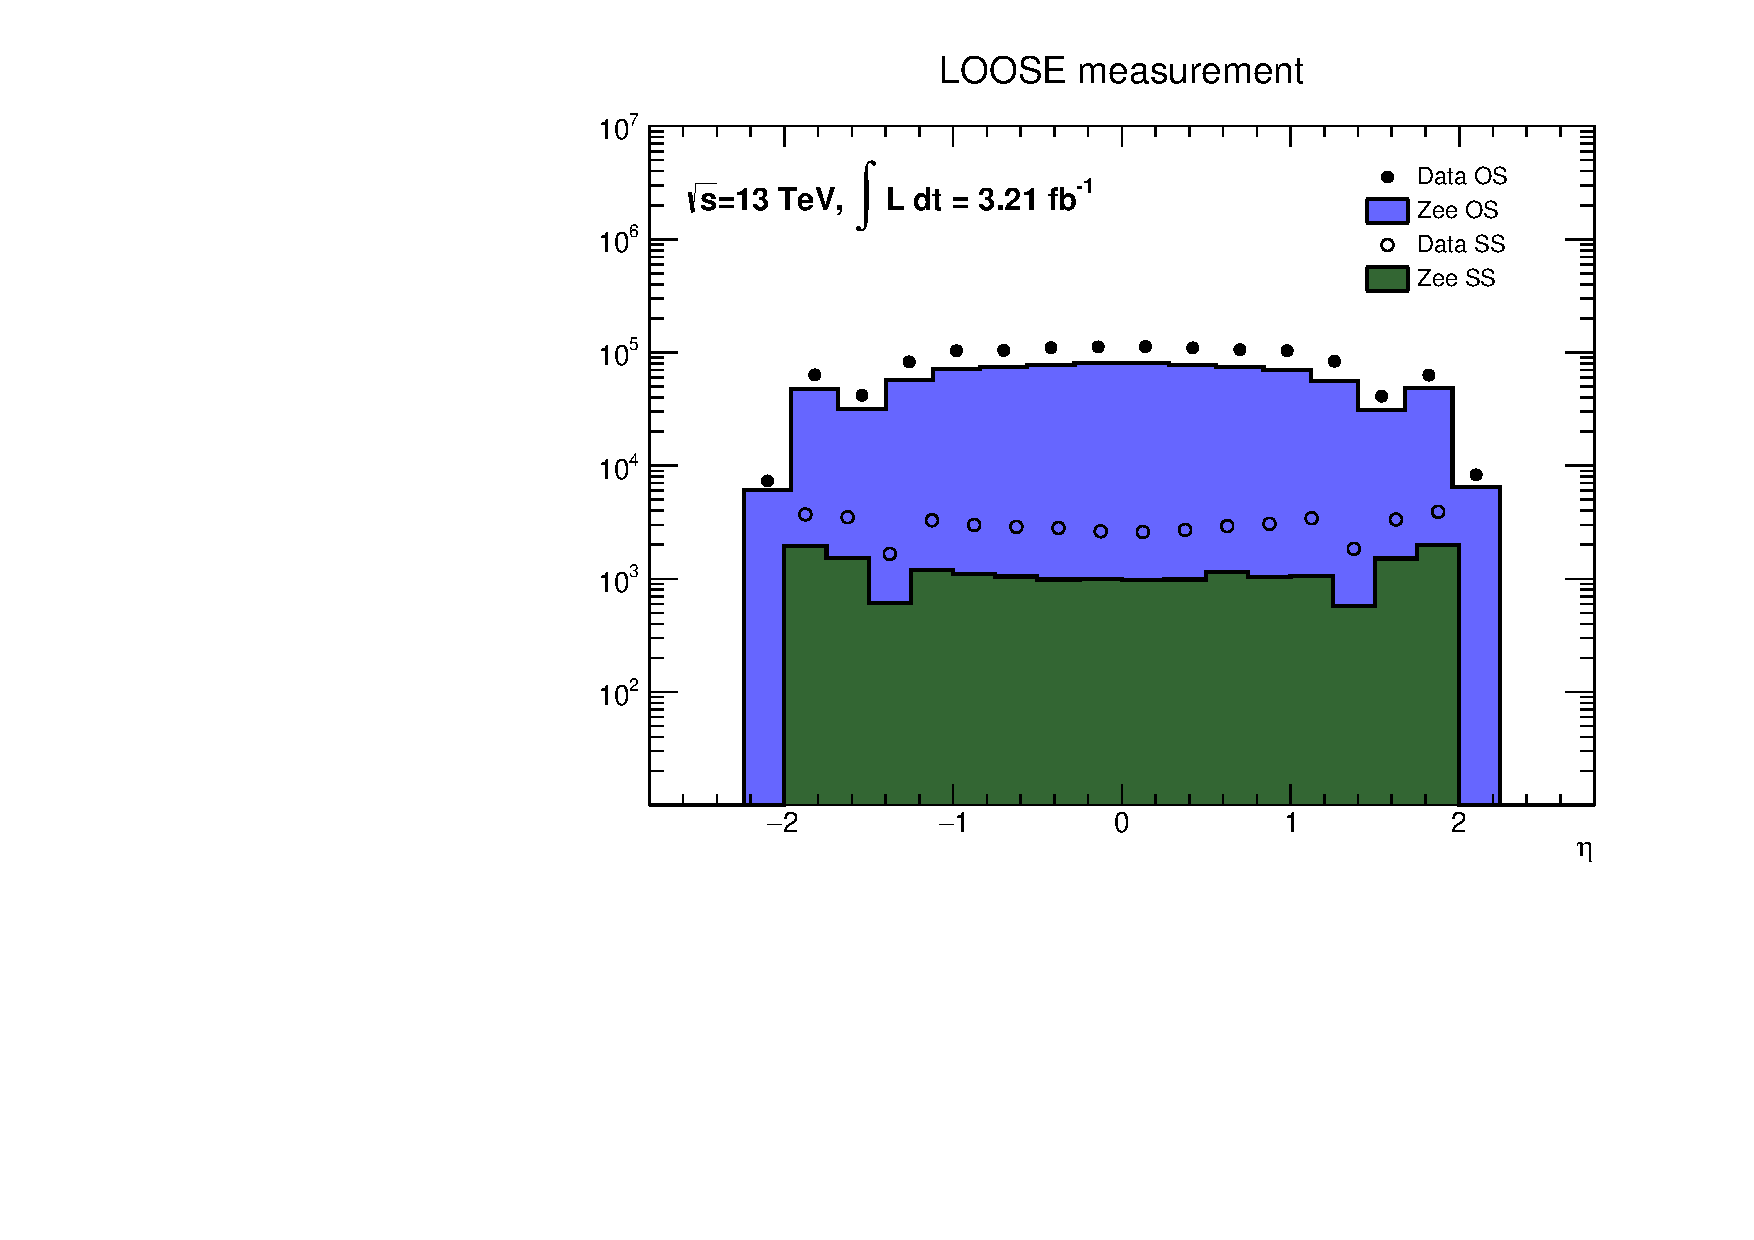
\includegraphics[width=0.4\textwidth]{FIGURES/BKG/chargeFlip/eta_loose_v28.pdf}
\caption{\label{fig:etasig} $\eta$ distributions for nominal (left) and loose (right) measurements for signal electrons forming an OS pair (filled dots for data, blue area for MC) and a SS pair (empty circles for data, green area for MC). Only statistical uncertainties are shown.}
\end{figure}
%------------------------------------------------


The invariant mass of electrons forming the pair is also an important quantity to look at and it is shown on Figure \ref{fig:mll}, where the left plot is the nominal measurement while the right plot correspond to the loose measurement. Again, the electrons forming an OS (black filled dots for data, blue area for MC) and a SS pair (black circle for data, green area for MC) are shown separately and the MC areas are normalized to data luminosity. The background is not subtracted in these plots.

%------------------------------------------------
\begin{figure}[!htb]
\centering
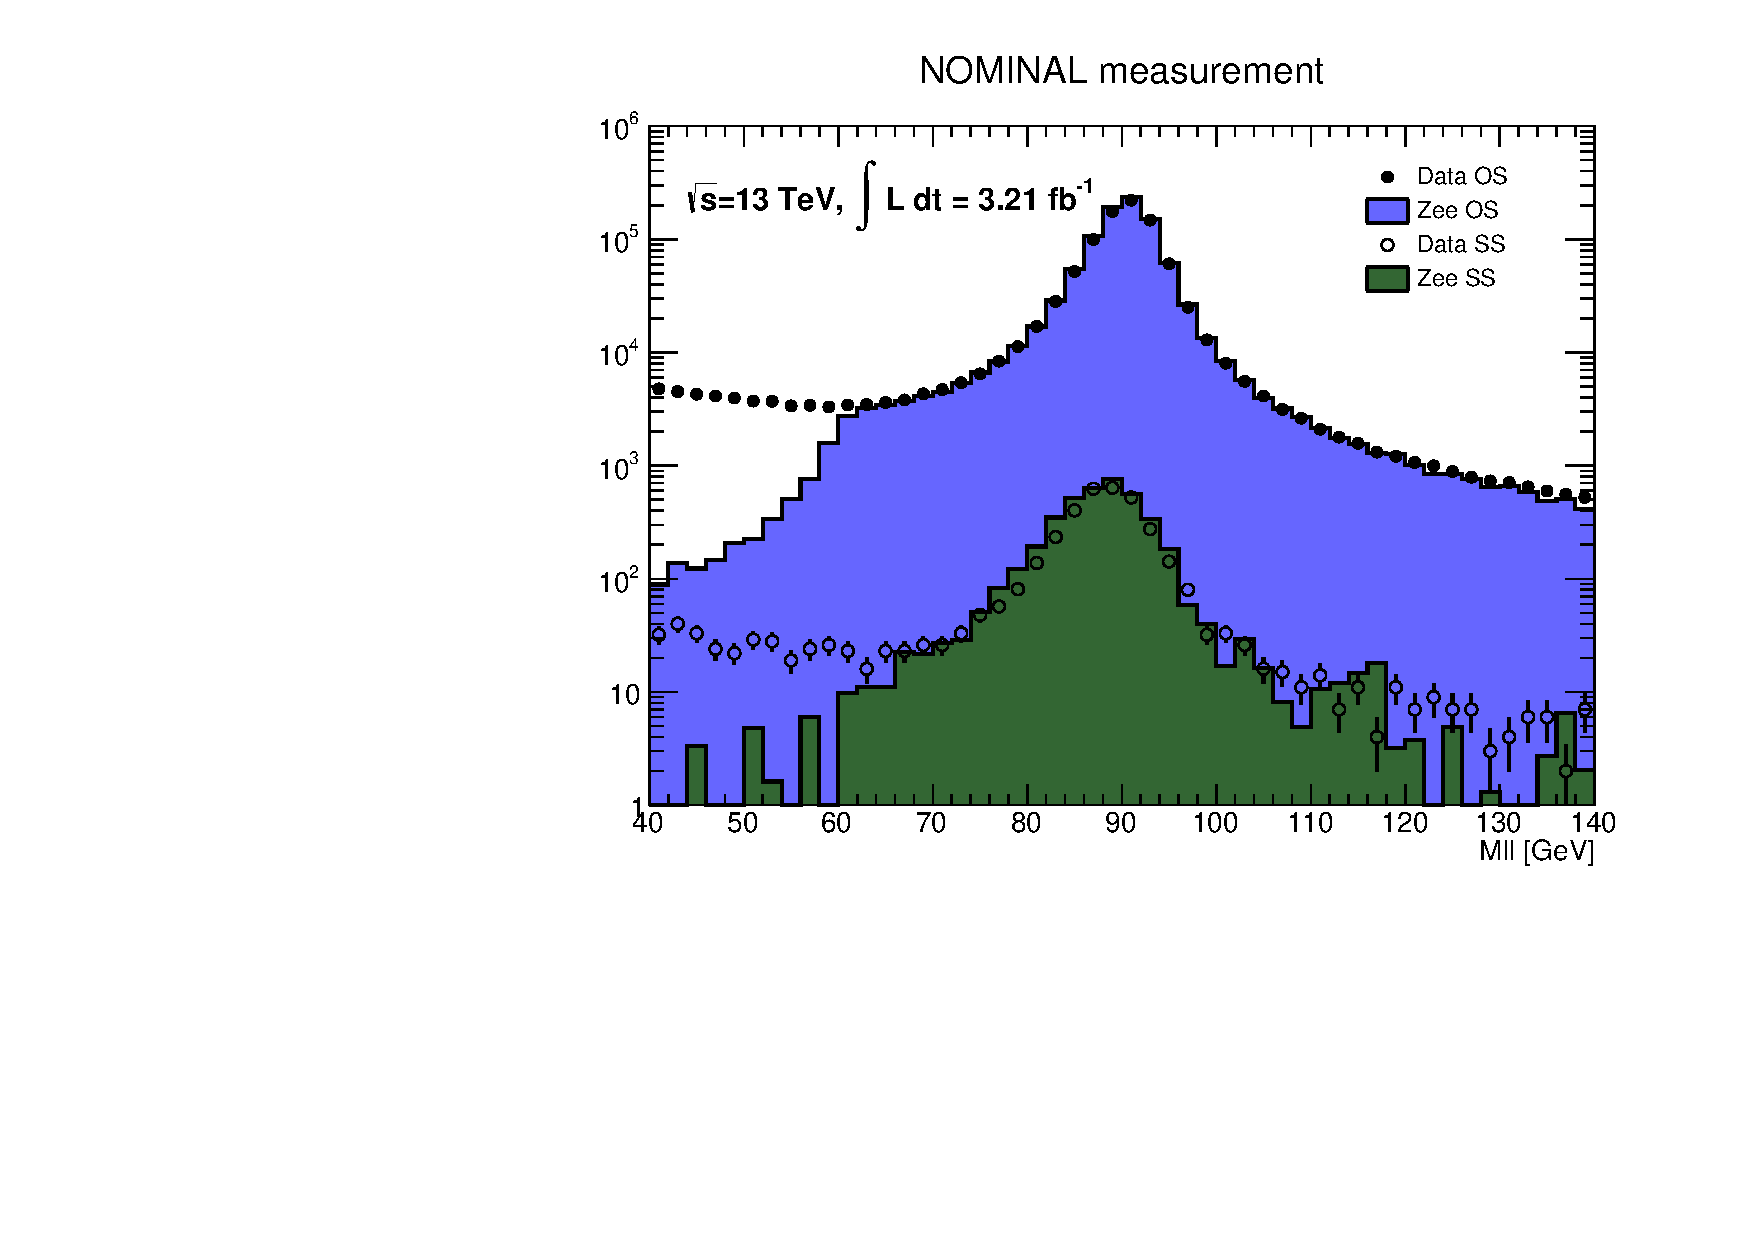
\includegraphics[width=0.4\textwidth]{FIGURES/BKG/chargeFlip/mll_nominal_v28.pdf}
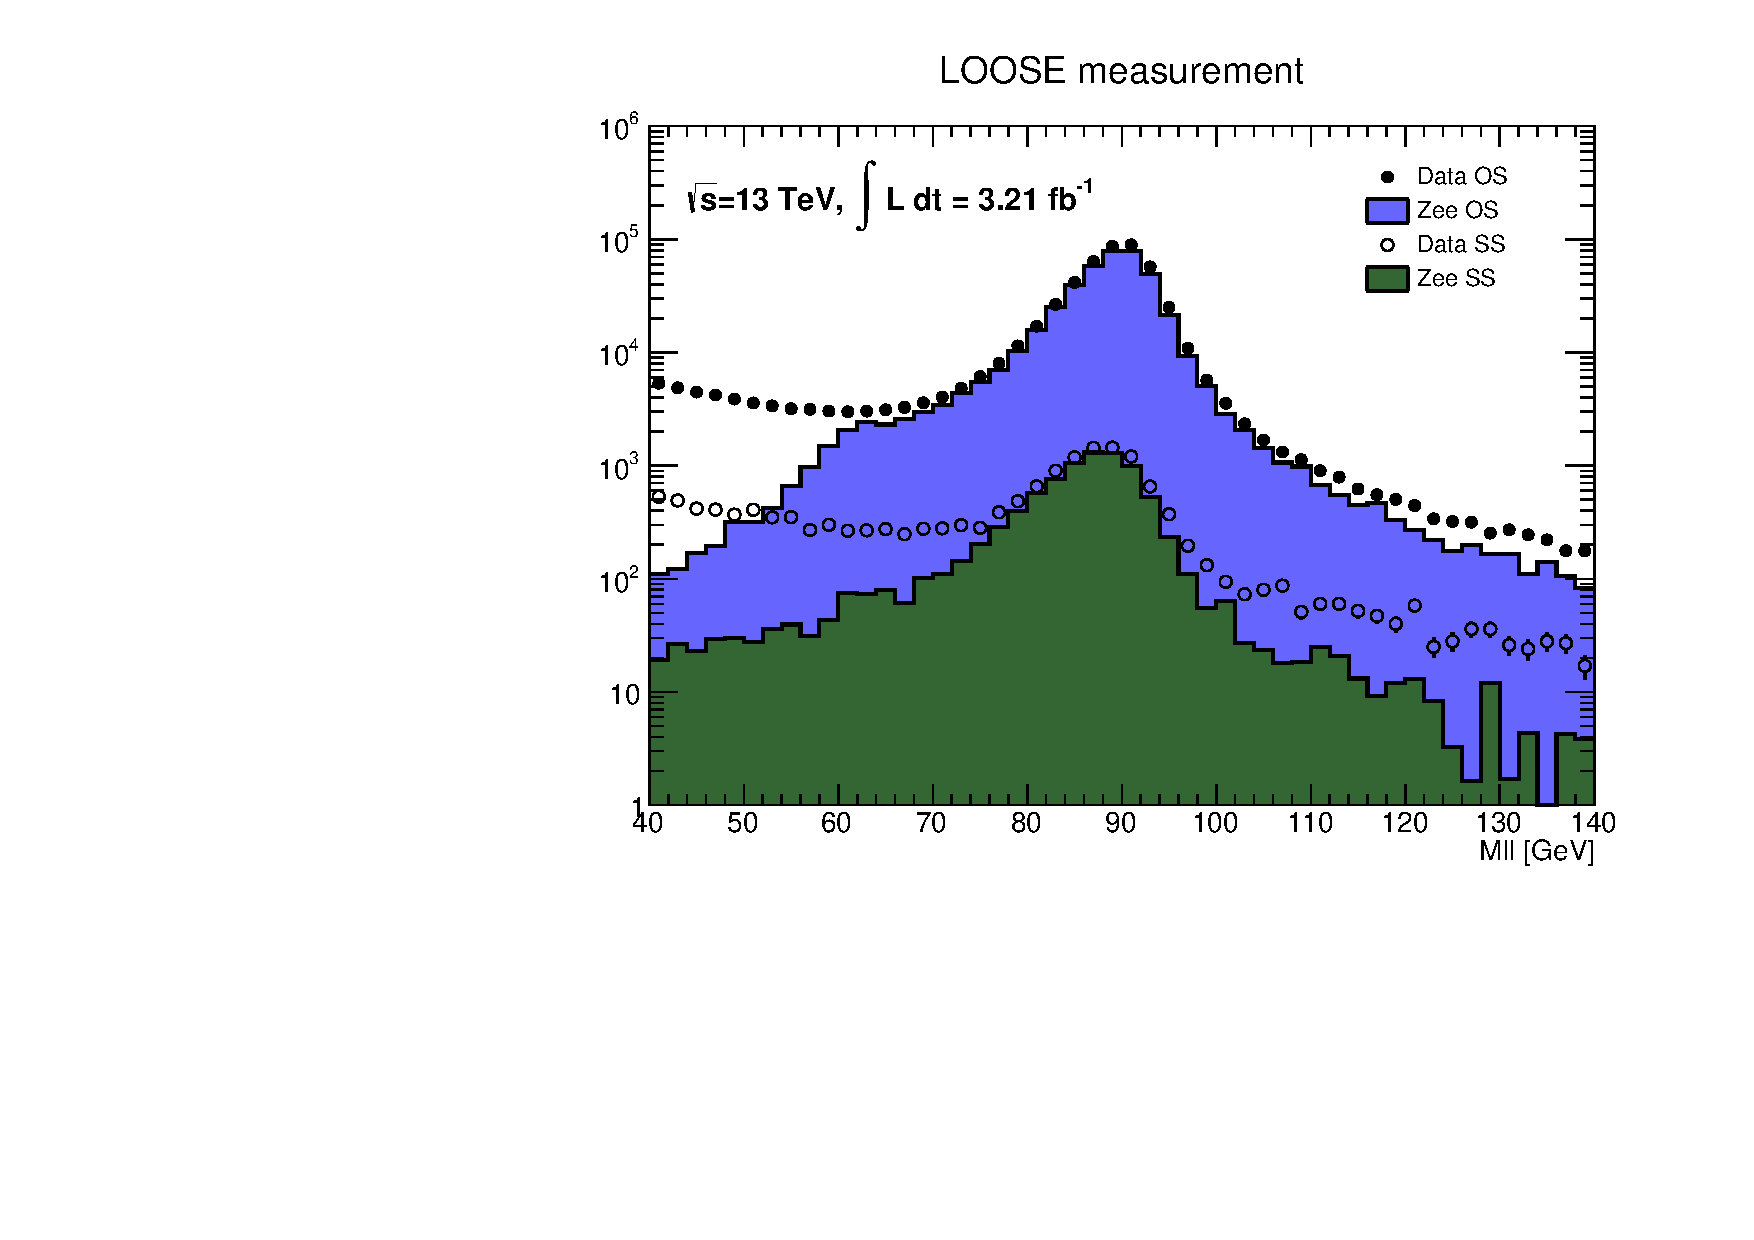
\includegraphics[width=0.4\textwidth]{FIGURES/BKG/chargeFlip/mll_loose_v28.pdf}
\caption{\label{fig:mll} Invariant mass distributions for nominal (left) and loose (right) measurements for signal electrons forming an OS pair (filled dots for data, blue area for MC) and a SS pair (empty circles for data, green area for MC). Only statistical uncertainties are shown.}
\end{figure}
%------------------------------------------------


Despite the small shift toward lower energies in the SS distribution, which is due to the loss of energy during the radiation process, 
one can see that there is a nice agreement between OS and SS pairs within the Z peak. 
Outside the peak, especially at low energy, one can see a large discrepancy in all distributions which comes from the fact 
that $Z\to e^+e^-$ was the only background considered. 
Again Drell-Yan processes and fake electrons (in the loose measurement cases) are the main causes of those differences. 
One can also see on Figure~\ref{fig:mll} that the amount of SS events (empty circles) for loose measurements is greater 
than the number of SS events in the nominal measurement while it is the opposite for the OS distributions (filled dots). 
This is expected since the cuts required to pass the signal requirements were designed to reject as much as possible detector backgrounds such as charge-flip electrons, 
so by requiring that one electron in the pair fails one of these requirements, the effect is clearly to raise the number of SS events and in the same time, 
lower the number of OS events. 
A background subtraction procedure using a side-band method is used to estimate the amount of background events in the measurement region. 
This method uses the number of observed events that fall in the side-band regions, $50<M_{ee}<75$~GeV and $100<M_{ee}<125$~GeV, 
to correct the number of events inside the central-band defined as $75<M_{ee}<100$~GeV. The systematic uncertainties related to those chosen values of central and side bands width are further discussed in the next section.


Finally, the nominal charge flip rates were computed following the procedures explained above for the following set of bins: $\pt$ bins = \{10, 20, 30, 40, 50, 60, 70, 80, 90, 100, 7000\} GeV, $|\eta|$ bins \{0.0, 0.8, 1.37, 2.0\}. In order to reduce the charge mis-identification background, events with an electron within the crack region ($1.37<|\eta|<1.52$) are vetoed as well as events where an electron from the pair has $|\eta|>2.0$. To be sure we got enough statistics in each bin, the number of electrons forming a SS events for the nominal and loose measurements are shown respectively on the top and bottom of Figure~\ref{fig:NSSdata}, where the higher $\pt$ bin contains the overflow. On those plots, one can see that most of the bins contain more than 20 electrons (except some bins at high $\pt$ values), which is enough to produce trustable charge flip rate results. By comparing those two figures, one can also see that the number of SS electrons ($N_{SS}$) is greater in the loose measurement case, but the distribution of $N_{SS}$ over the bins is similar between both measurements.

%-----------------------------------------------
\begin{figure}[!htb]
\centering
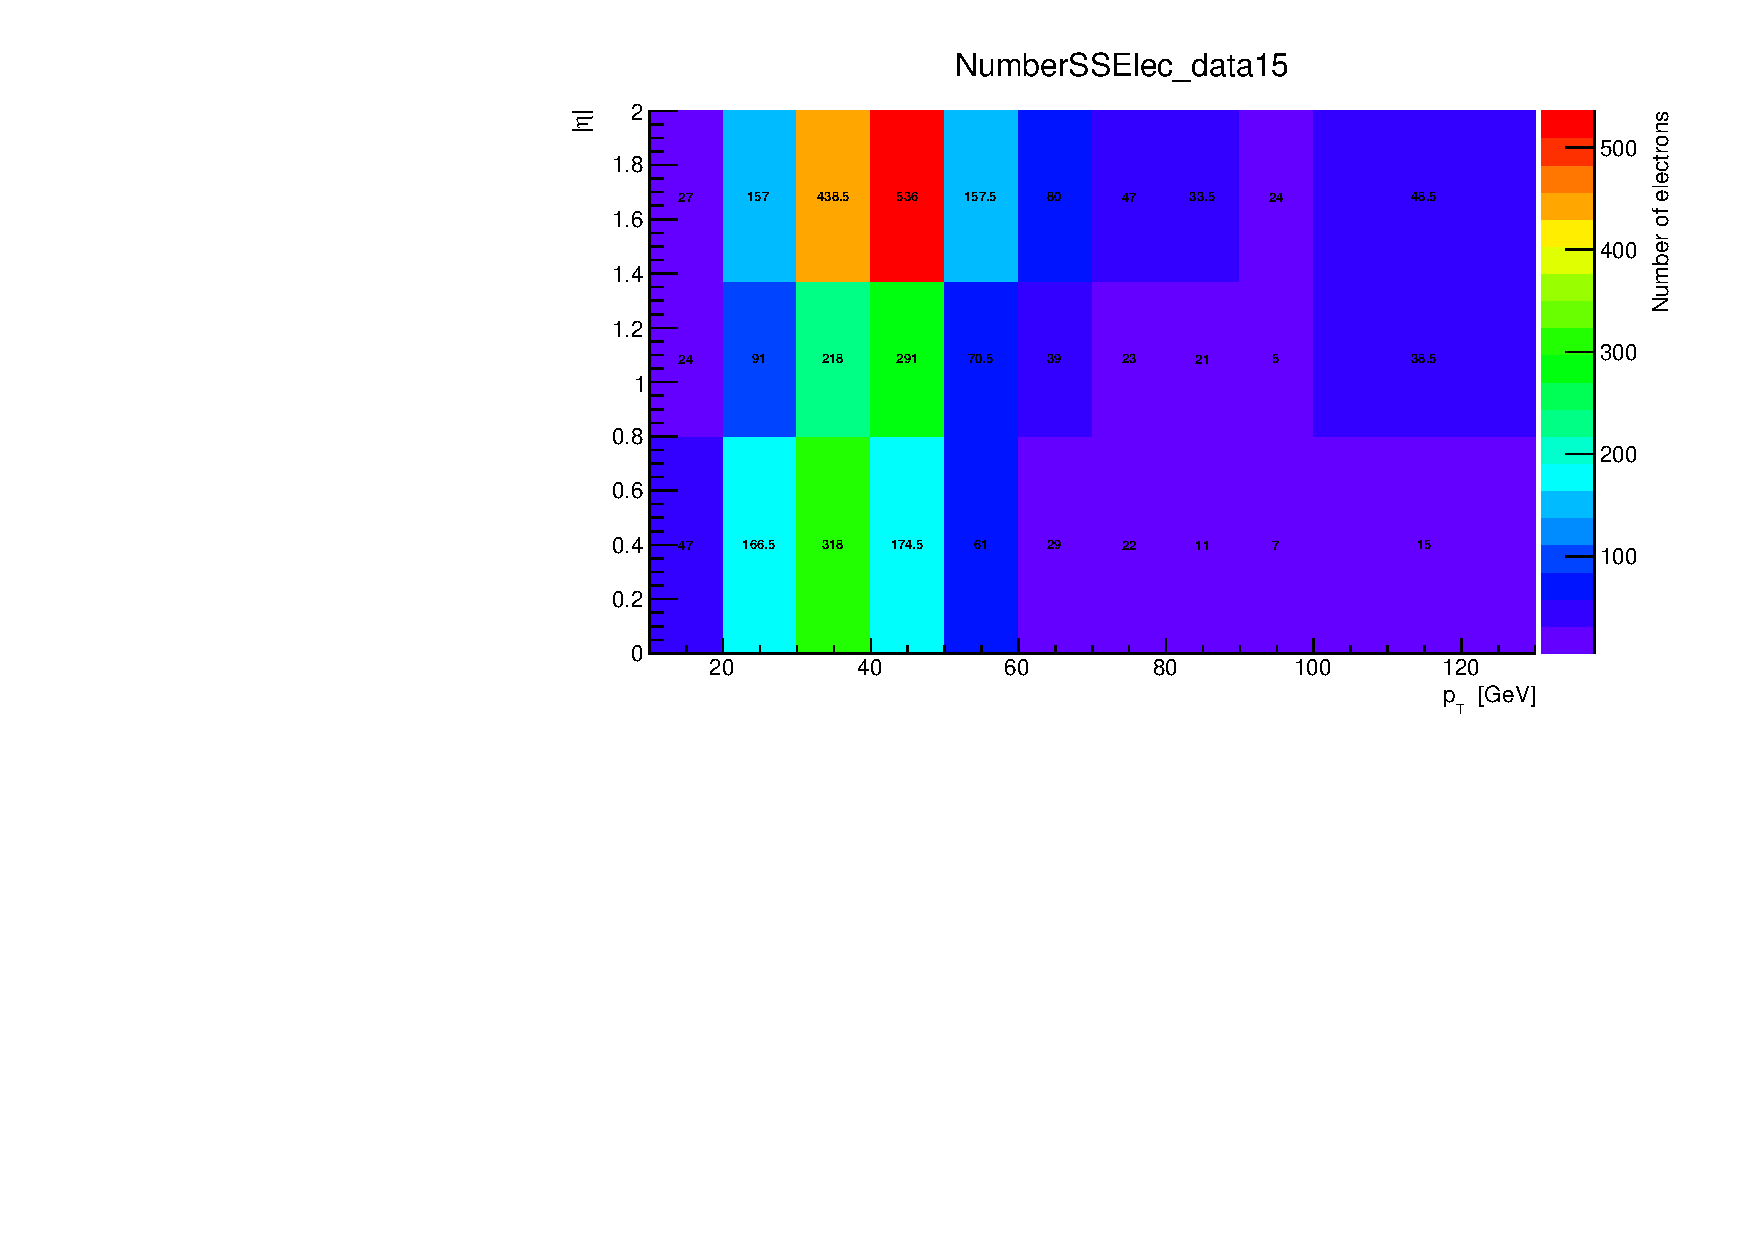
\includegraphics[width=0.65\textwidth]{FIGURES/BKG/chargeFlip/2D_histo_NumberSSElec_data15.pdf}
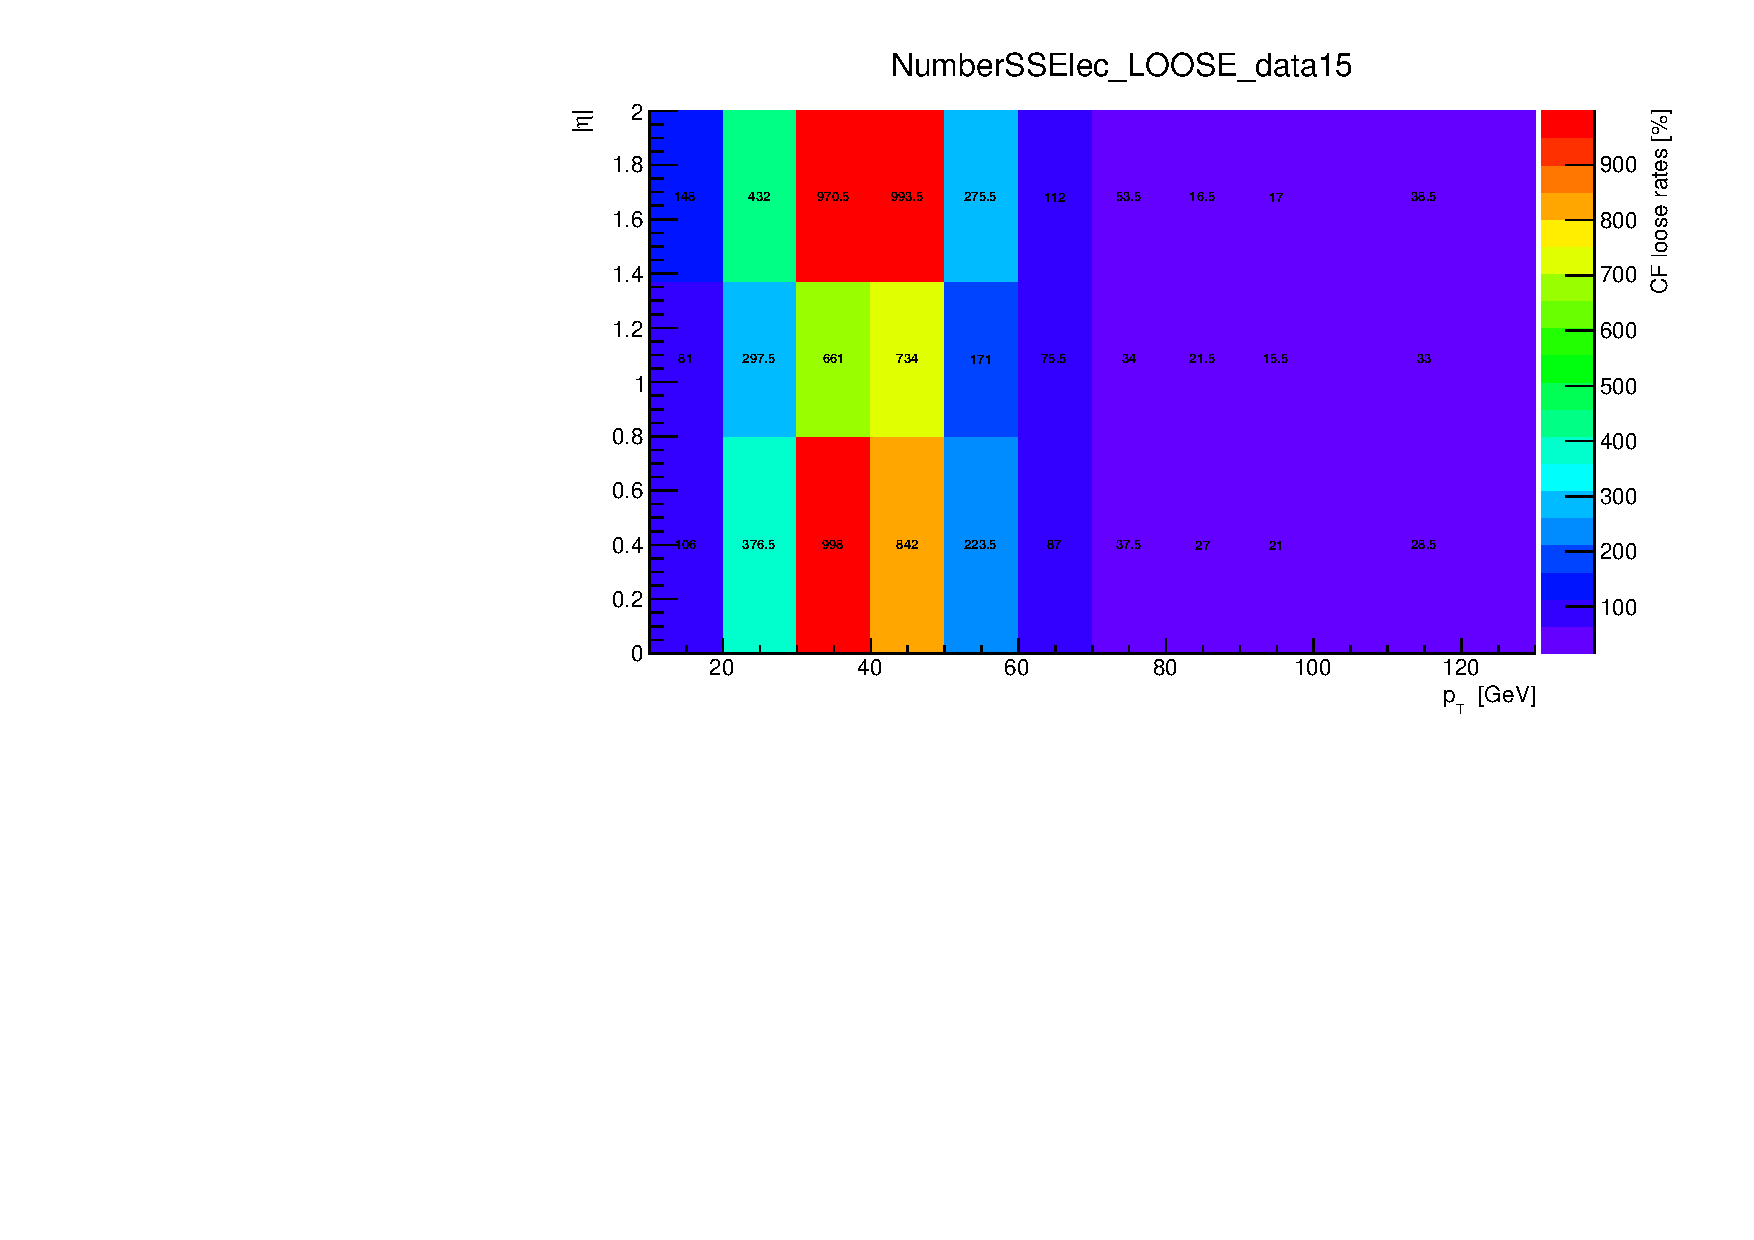
\includegraphics[width=0.65\textwidth]{FIGURES/BKG/chargeFlip/2D_histo_NumberSSElec_LOOSE_data15.pdf}
\caption{\label{fig:NSSdata} Number of electrons which form a same-sign event in 40 ($pt , | \eta | $) bins, used to compute the charge flip rates for the NOMINAL (top) and LOOSE (bottom) measurement  extracted from data, where the higher $\pt$ bins contain the overflow.}
\end{figure}
%------------------------------------------------

The nominal and loose rates extracted with data samples are presented respectively on Figure~\ref{fig:CFdata} extracted in data, where the higher $\pt$ bins contain the overflow. On Figure~\ref{fig:CFdata}, one can see that the expected trend, charge flip rate values are greater for higher $\pt$ and $\eta$ bins, is confirmed. On the top plot, the nominal measurement goes up to 0.75\% in the barrel region ($0.0<|\eta|<1.37$) while it goes up to 3.7\% in region $1.52<|\eta|<2.0$. On the bottom plot, the loose measurements are in general greater than the nominal ones in every bins and the rates goes up to 7.4\% in the barrel region ($0.0<|\eta|<1.37$) while it goes up to 10.8\% in region $1.52<|\eta|<2.0$. Another way to observe the charge flip dependancy on $\pt$ and $\eta$ is to plot all the rates on the same figures in function of $\pt$ as shown on Figure~\ref{fig:CFvsPt} where the $0.0<|\eta|<0.8$ range are shown in blue, the $0.8<|\eta|<1.37$ range in green and the $1.37<|\eta|<2.0$ range in orange. Despite some variations for the loose measurement in high $\pt$ bins, one can see that charge flip rates become greater when the $\pt$ value, as well as the $\eta$ value, increases.

%------------------------------------------------
\begin{figure}[!htb]
\centering
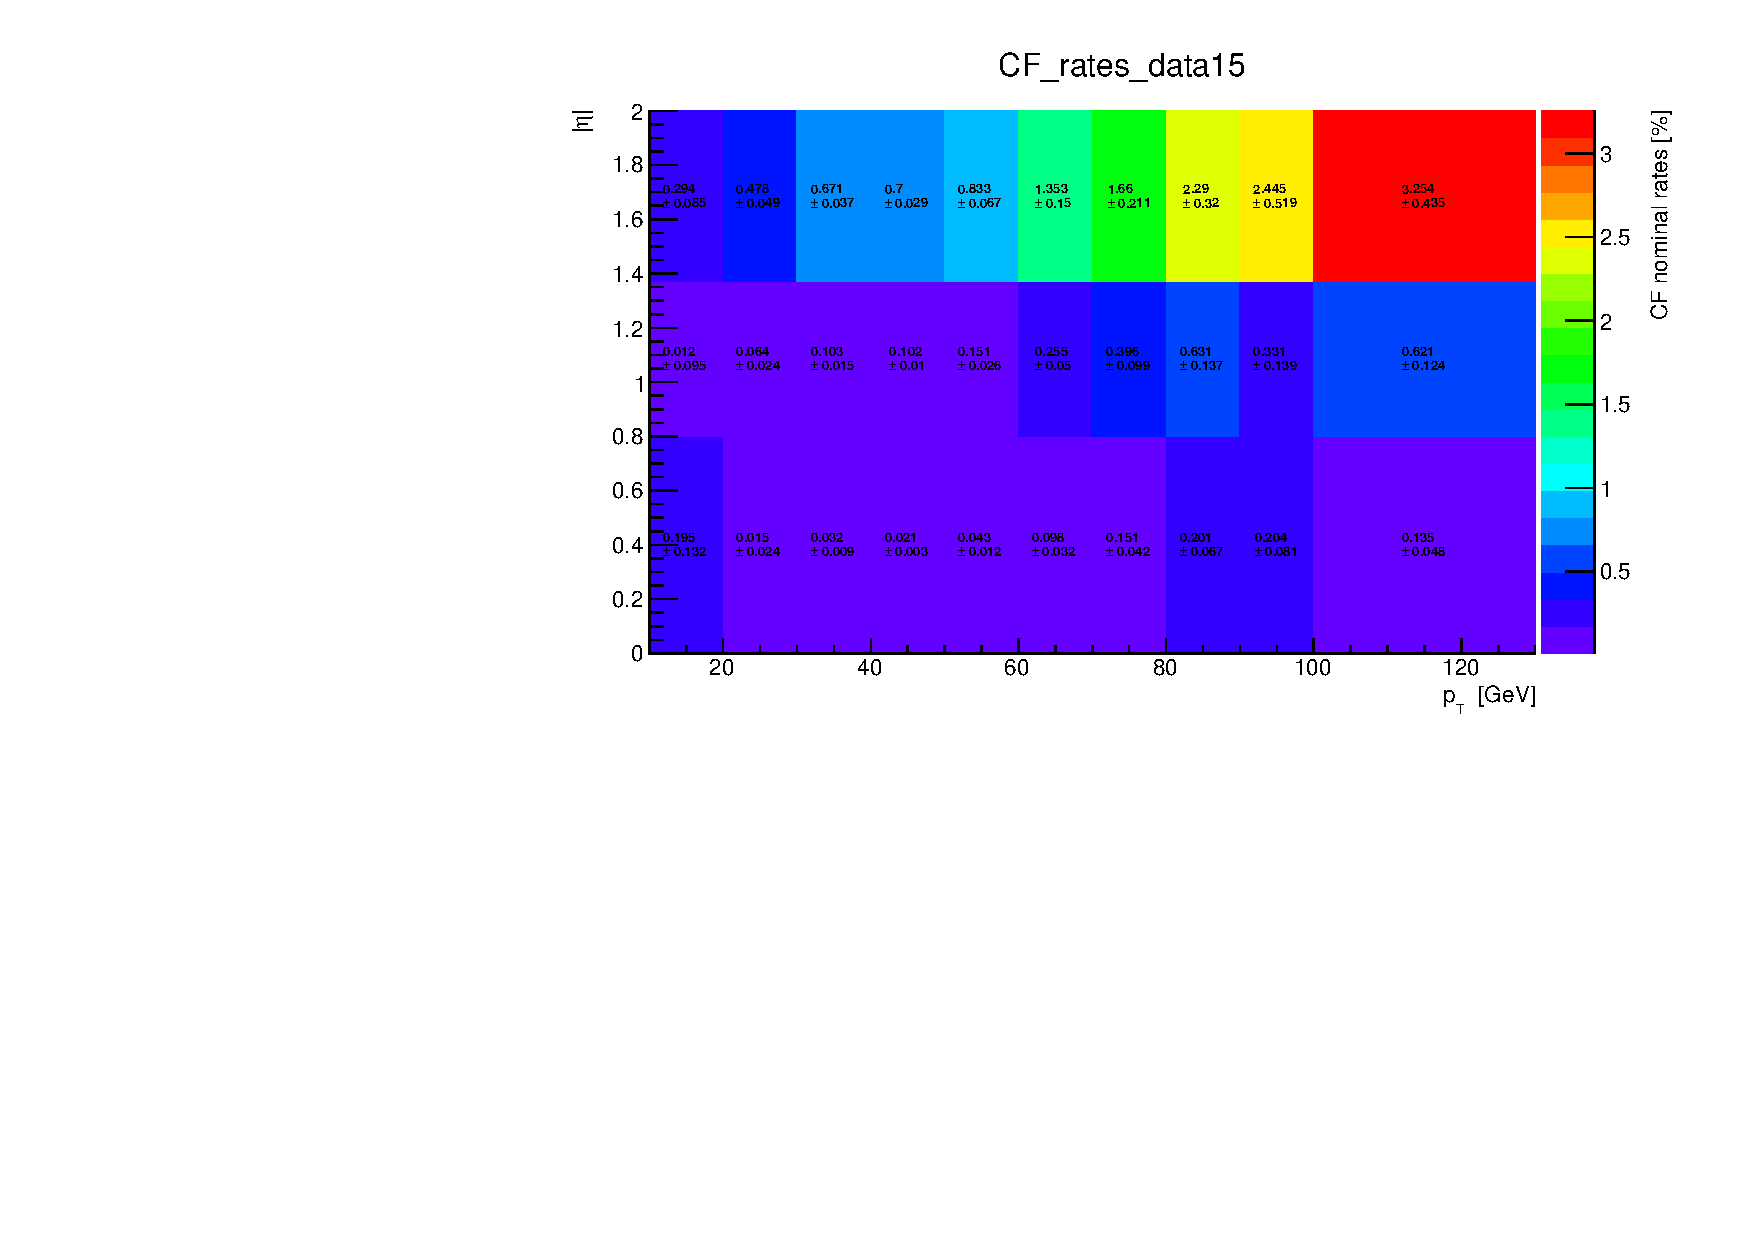
\includegraphics[width=0.65\textwidth]{FIGURES/BKG/chargeFlip/2D_histo_CF_rates_data15.pdf}

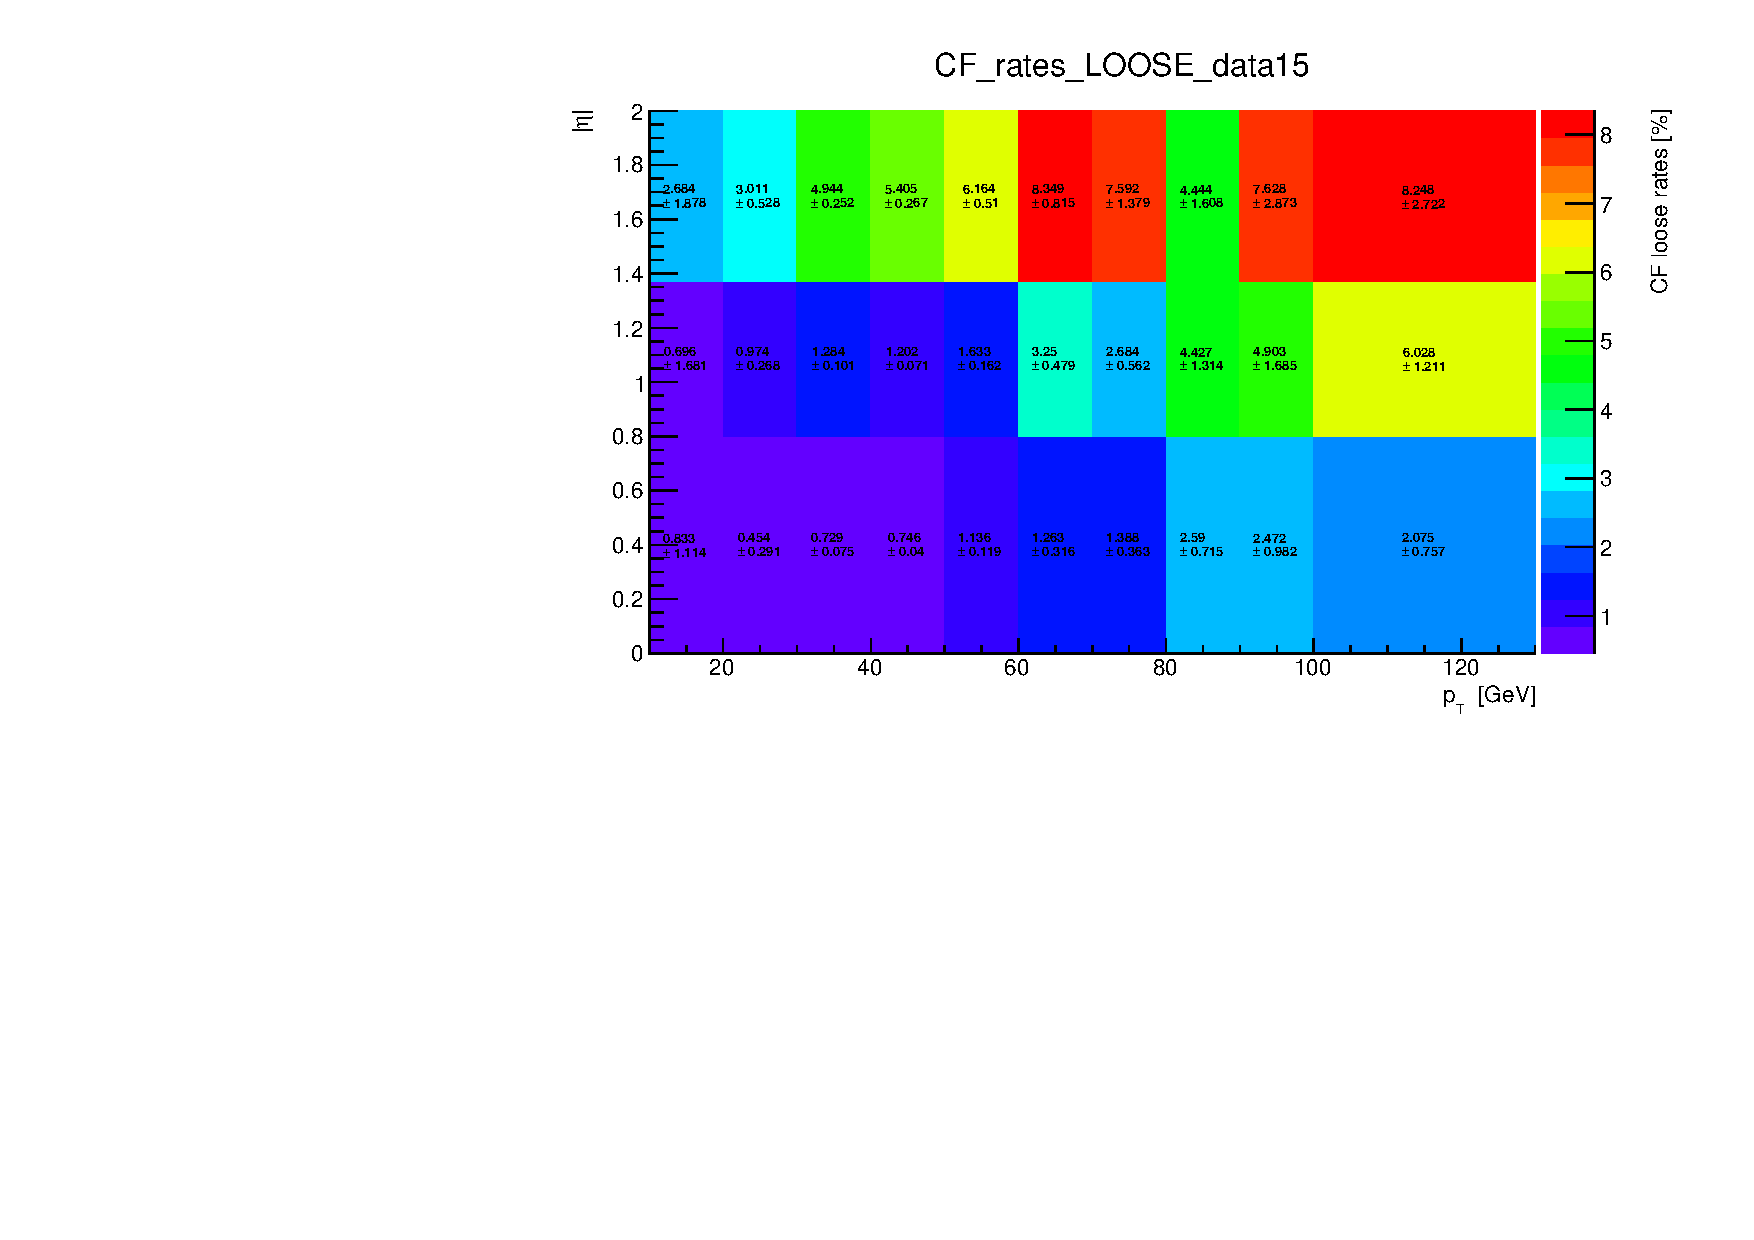
\includegraphics[width=0.65\textwidth]{FIGURES/BKG/chargeFlip/2D_histo_CF_rates_LOOSE_data15.pdf}
\caption{\label{fig:CFdata} Mis-identification rates in 40 ($pt , |\eta| $) bins with their respective statistical+systematic uncertainties for the NOMINAL (top) and LOOSE (bottom) measurement extracted in data, where the higher $\pt$ bins contain the overflow.}
\end{figure}
%------------------------------------------------

%------------------------------------------------
\begin{figure}[!htb]
\centering
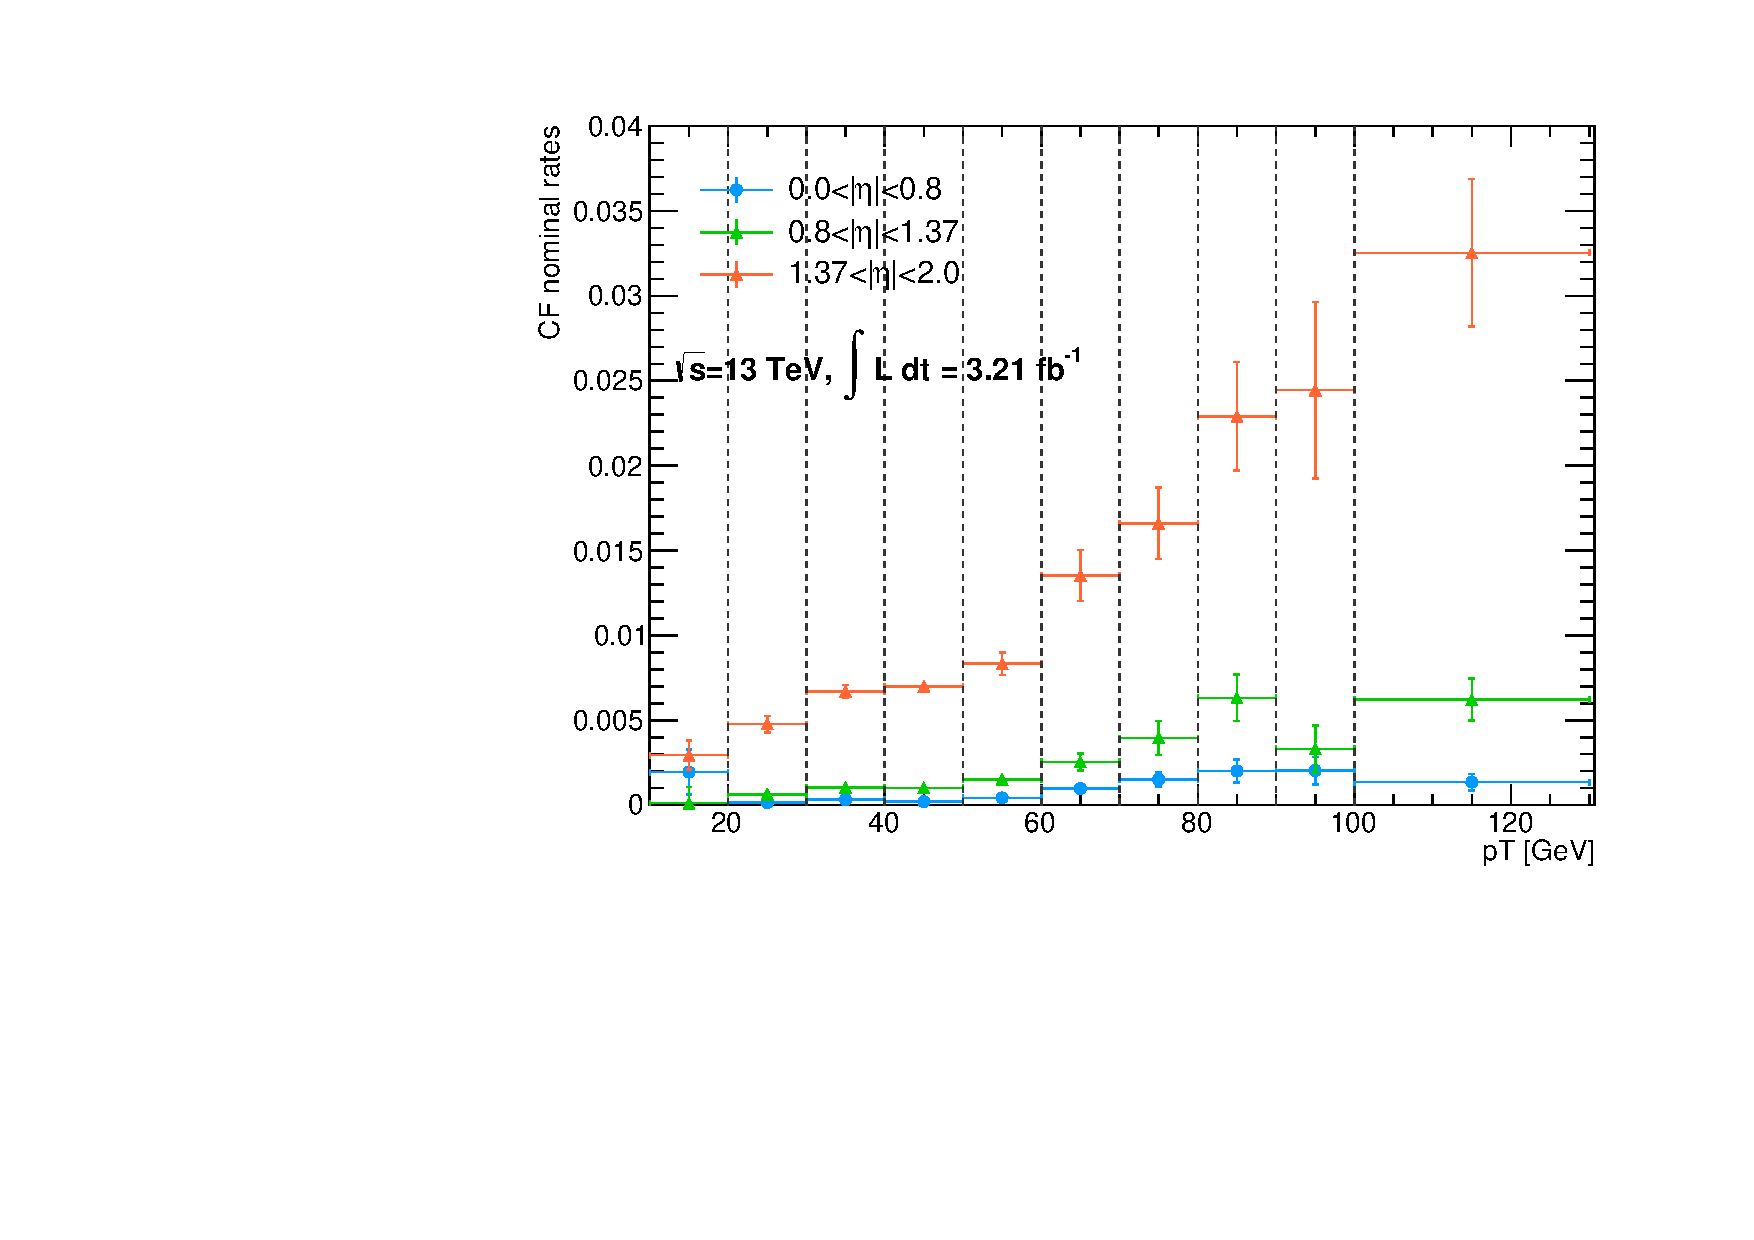
\includegraphics[width=0.65\textwidth]{FIGURES/BKG/chargeFlip/CFratesVSpt_data15.pdf}

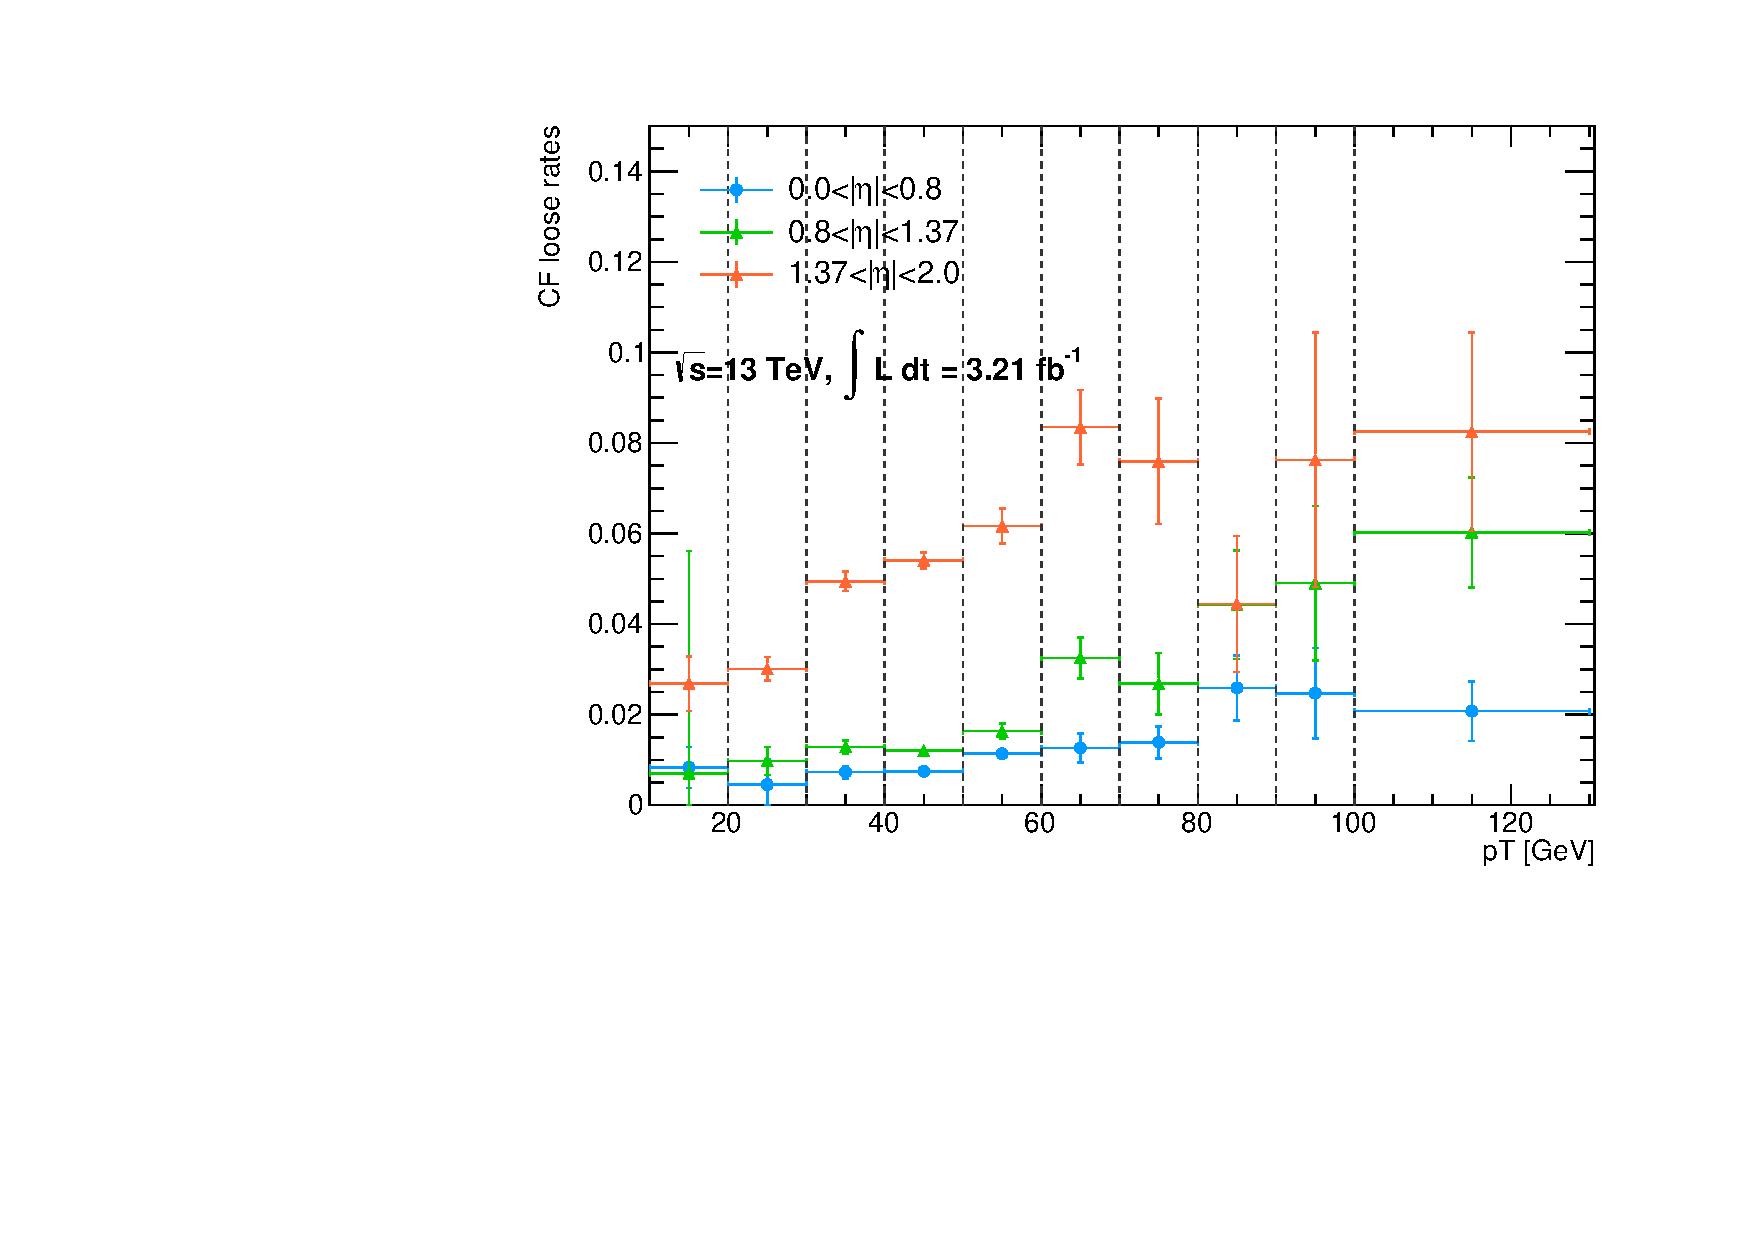
\includegraphics[width=0.65\textwidth]{FIGURES/BKG/chargeFlip/CFratesVSpt_LOOSE_data15.pdf}
\caption{\label{fig:CFvsPt} Mis-identification rates in function of the $\pt$ distribution for three different $\eta$ ranges: $0.0<|\eta|<0.8$ in blue, $0.8<|\eta|<1.37$ in green and $1.37<|\eta|<2.0$ in orange. Statistical and systematic uncertainties are include. The top (bottom) plot show nominal (loose) measurement extracted in data, where the higher $\pt$ bin contains the overflow.}
\end{figure}
%------------------------------------------------


The comparison of charge flip rates from data and from MC for nominal measurement is plotted for different $\pt$ range on Figure~\ref{fig:CFratesNominal_1}. The same comparison was done for the loose measurement, it is shown on Figure~\ref{fig:CFratesLoose_2} and are notably used in section~\ref{sec:bkg_VP_DD_estimates}. Again, one can see that the charge flip rates for the loose measurement are much larger than for the nominal measurement (typically by a factor 10), illustrating the necessity of this auxiliary measurement. From those plots, one can see a fairly good agreement between data and MC results. In low $\pt$ bins (below 40 GeV) in the nominal measurement, MC predictions seem to overestimate the charge flip rates at high $|\eta|$ ($1.52<|\eta|<2.0$). For the loose measurement, the same pattern appear in high $\pt$ region (above 60 GeV) in the last $|\eta|$ bin where one can see that MC predictions overestimate the charge flip rates obtained from data sample. Apart those small differences, the agreement between data and MC is good in general.

%------------------------------------------------
\begin{figure}[h!]
\centering
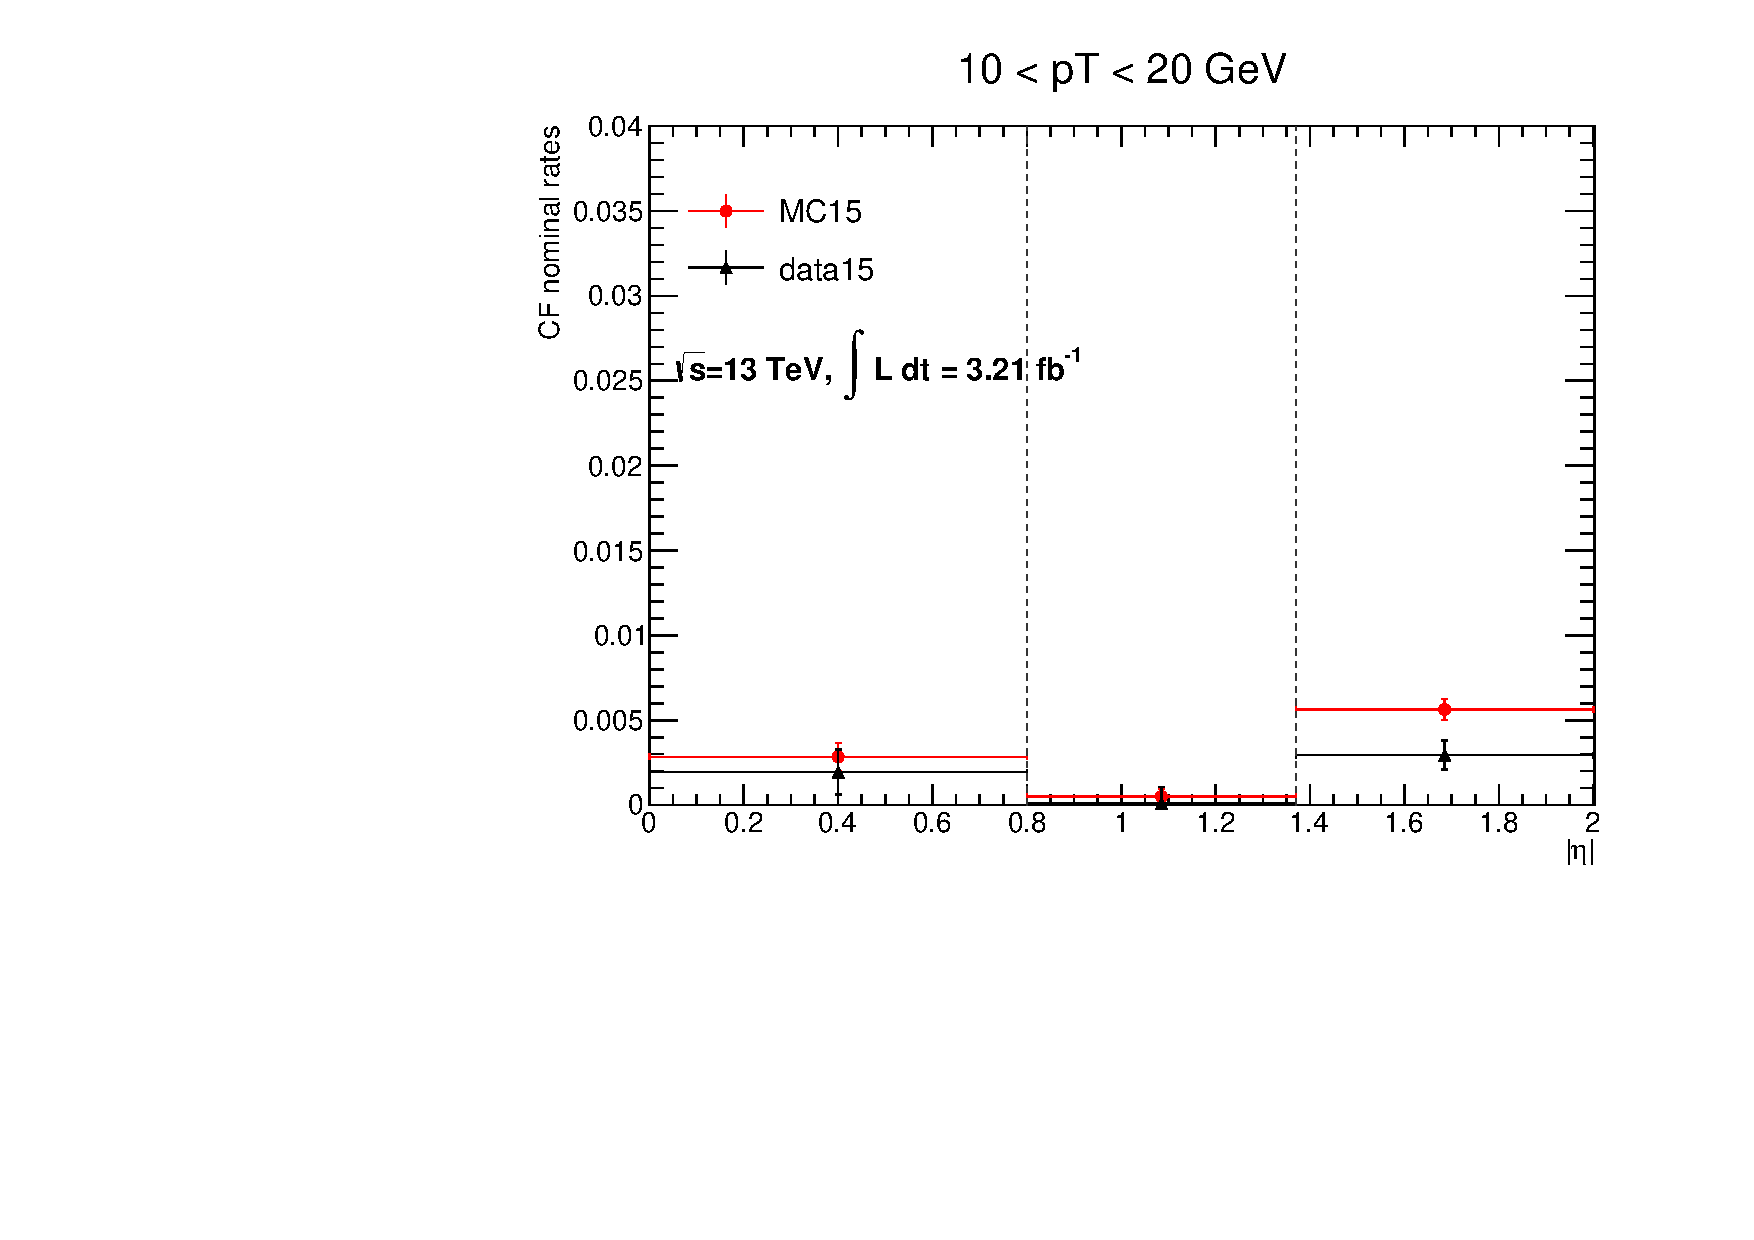
\includegraphics[width=0.4\textwidth]{FIGURES/BKG/chargeFlip/CFrates___dataVSmc___PTbin0.pdf}
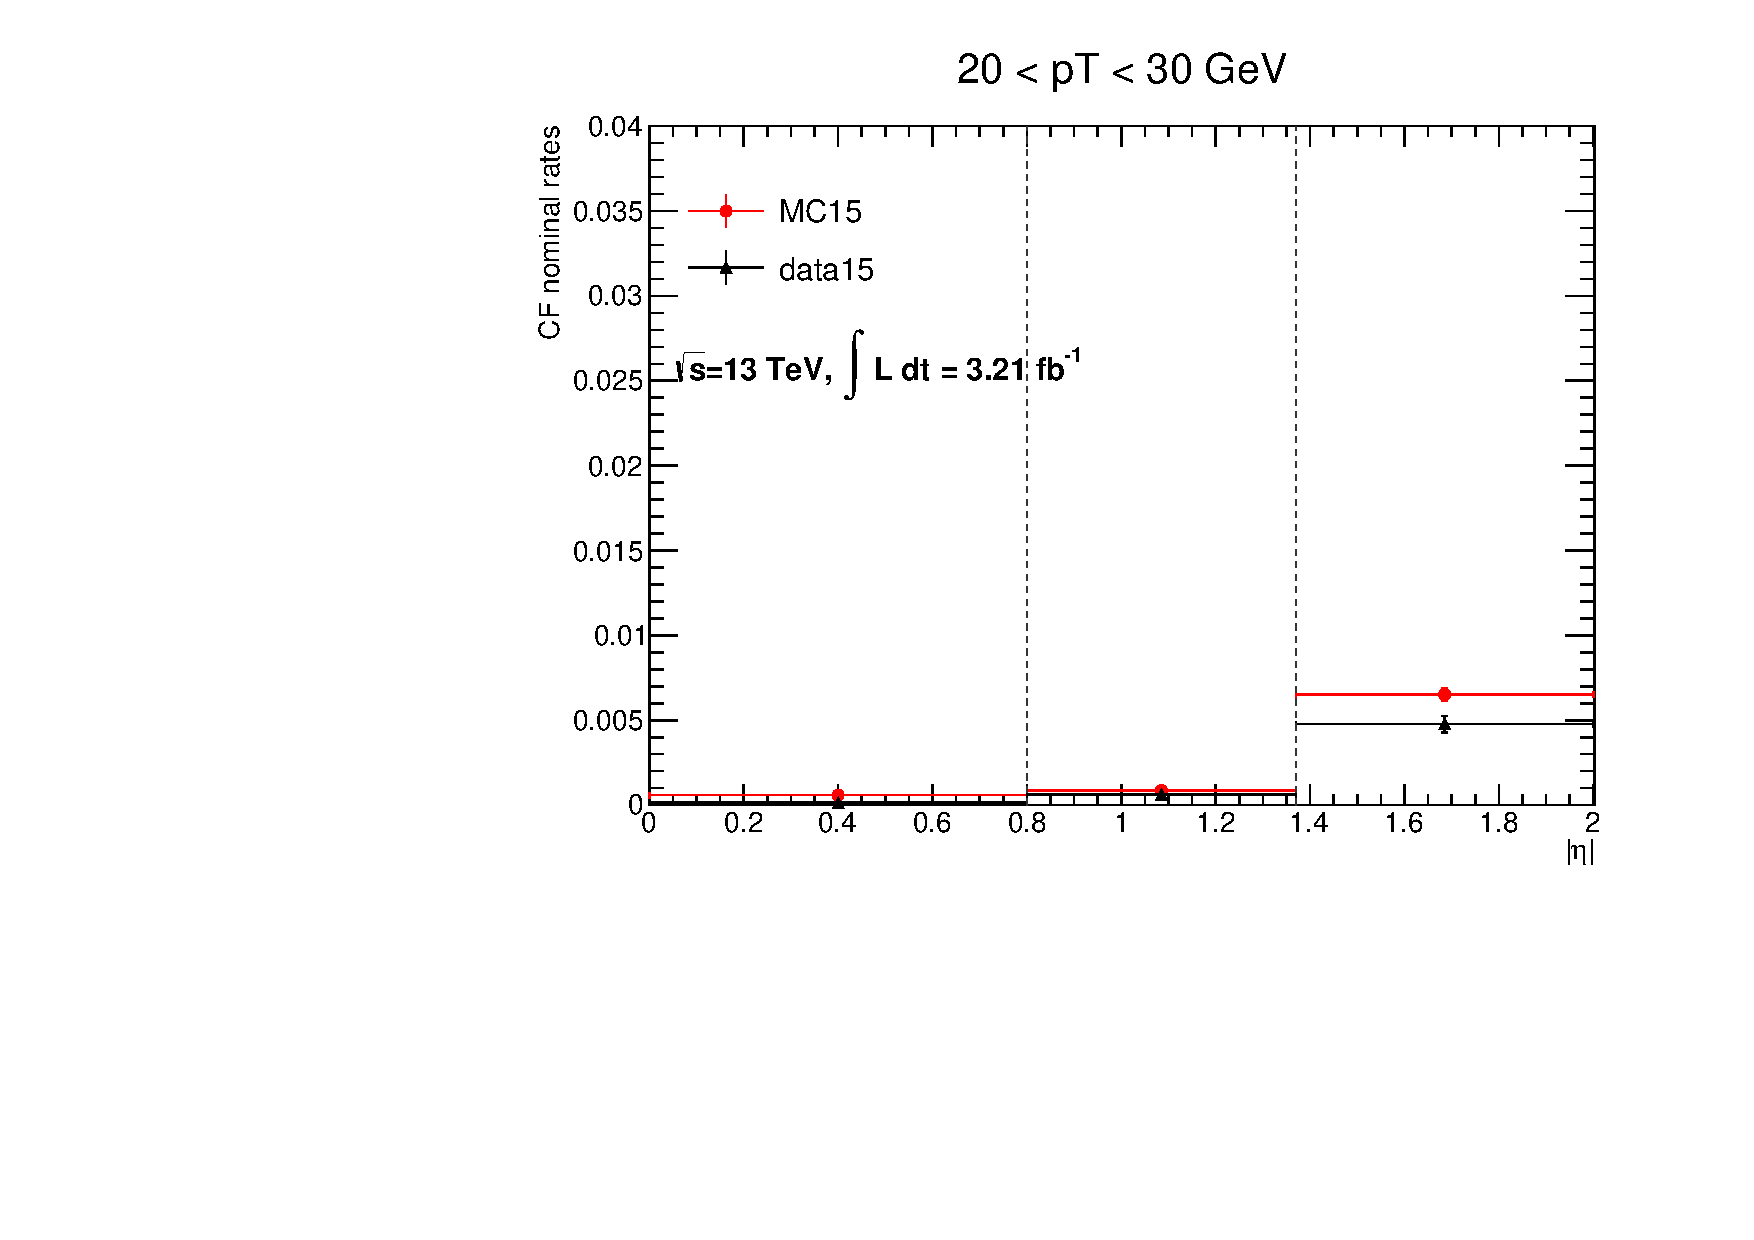
\includegraphics[width=0.4\textwidth]{FIGURES/BKG/chargeFlip/CFrates___dataVSmc___PTbin1.pdf}
\vfill
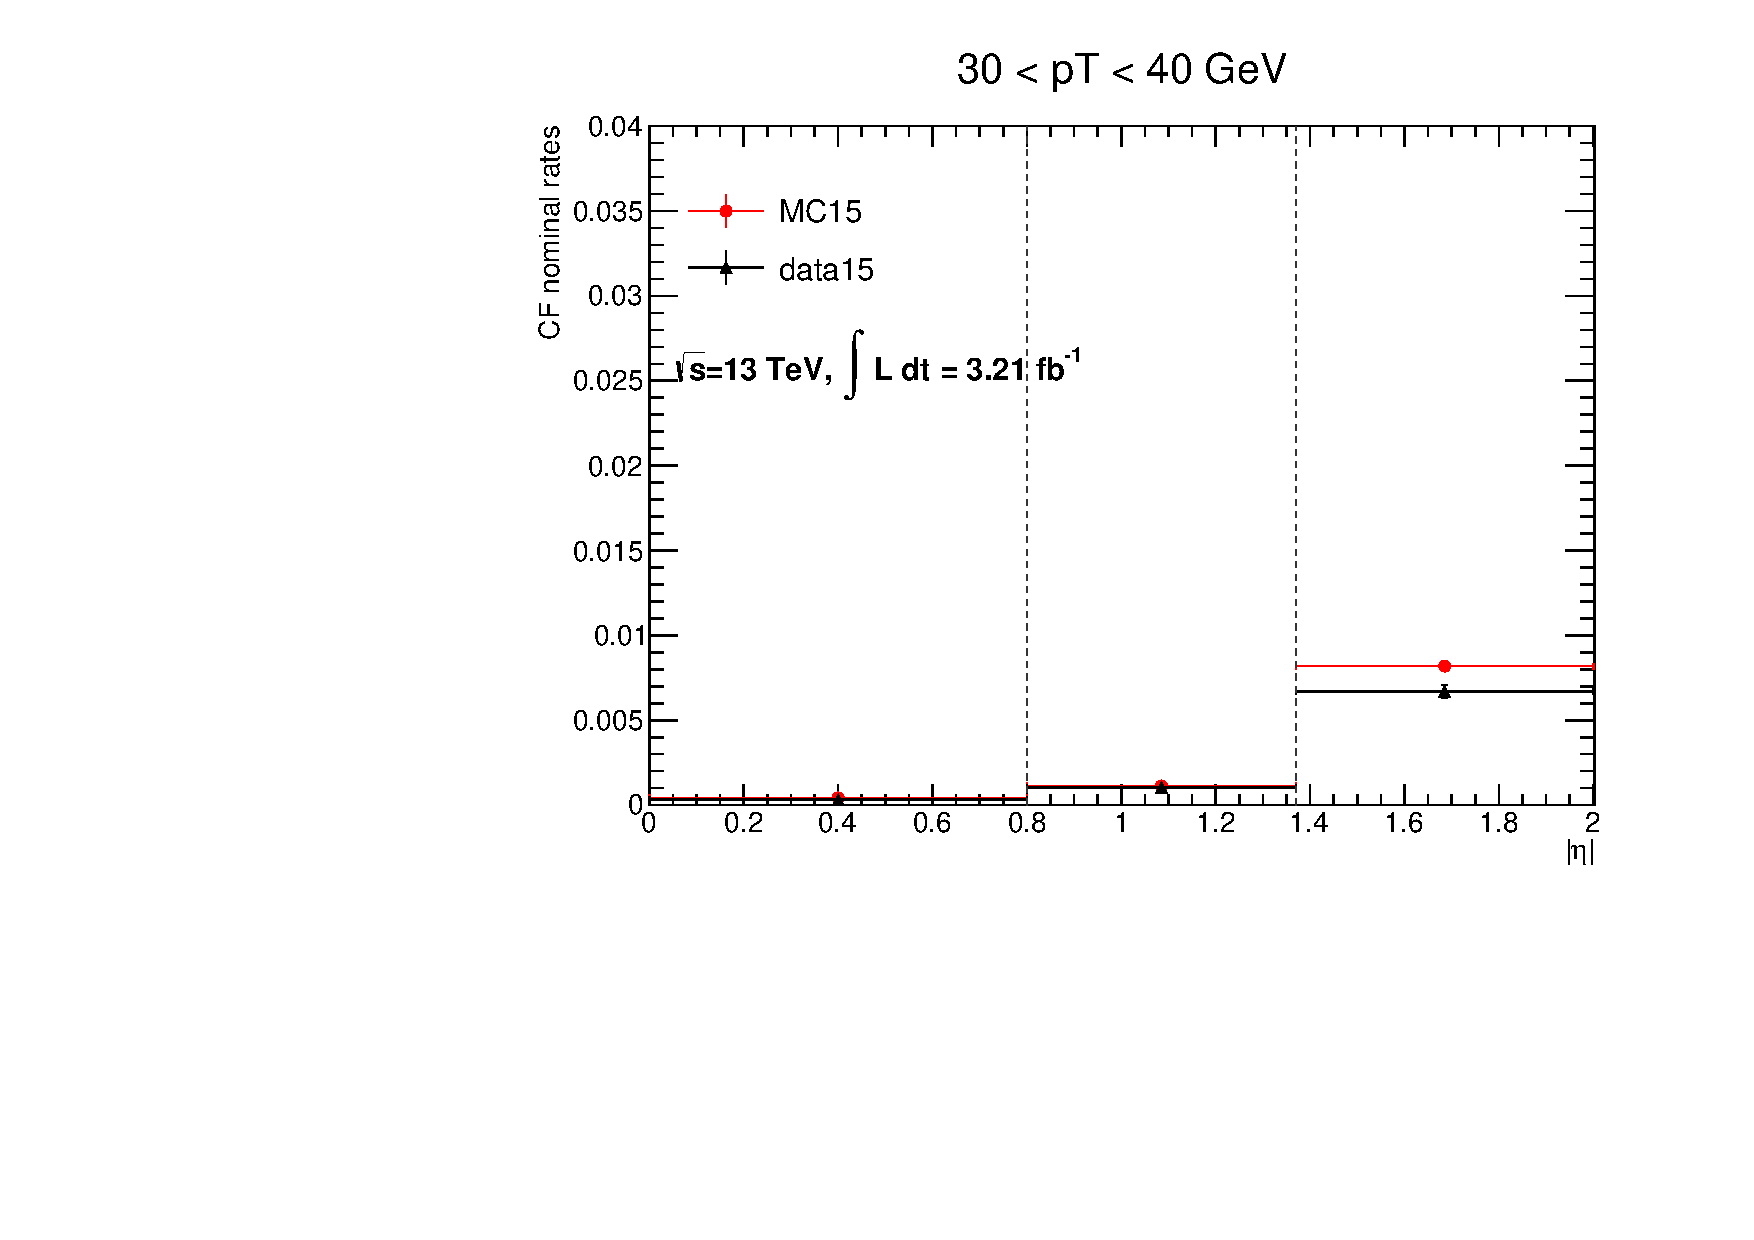
\includegraphics[width=0.4\textwidth]{FIGURES/BKG/chargeFlip/CFrates___dataVSmc___PTbin2.pdf}
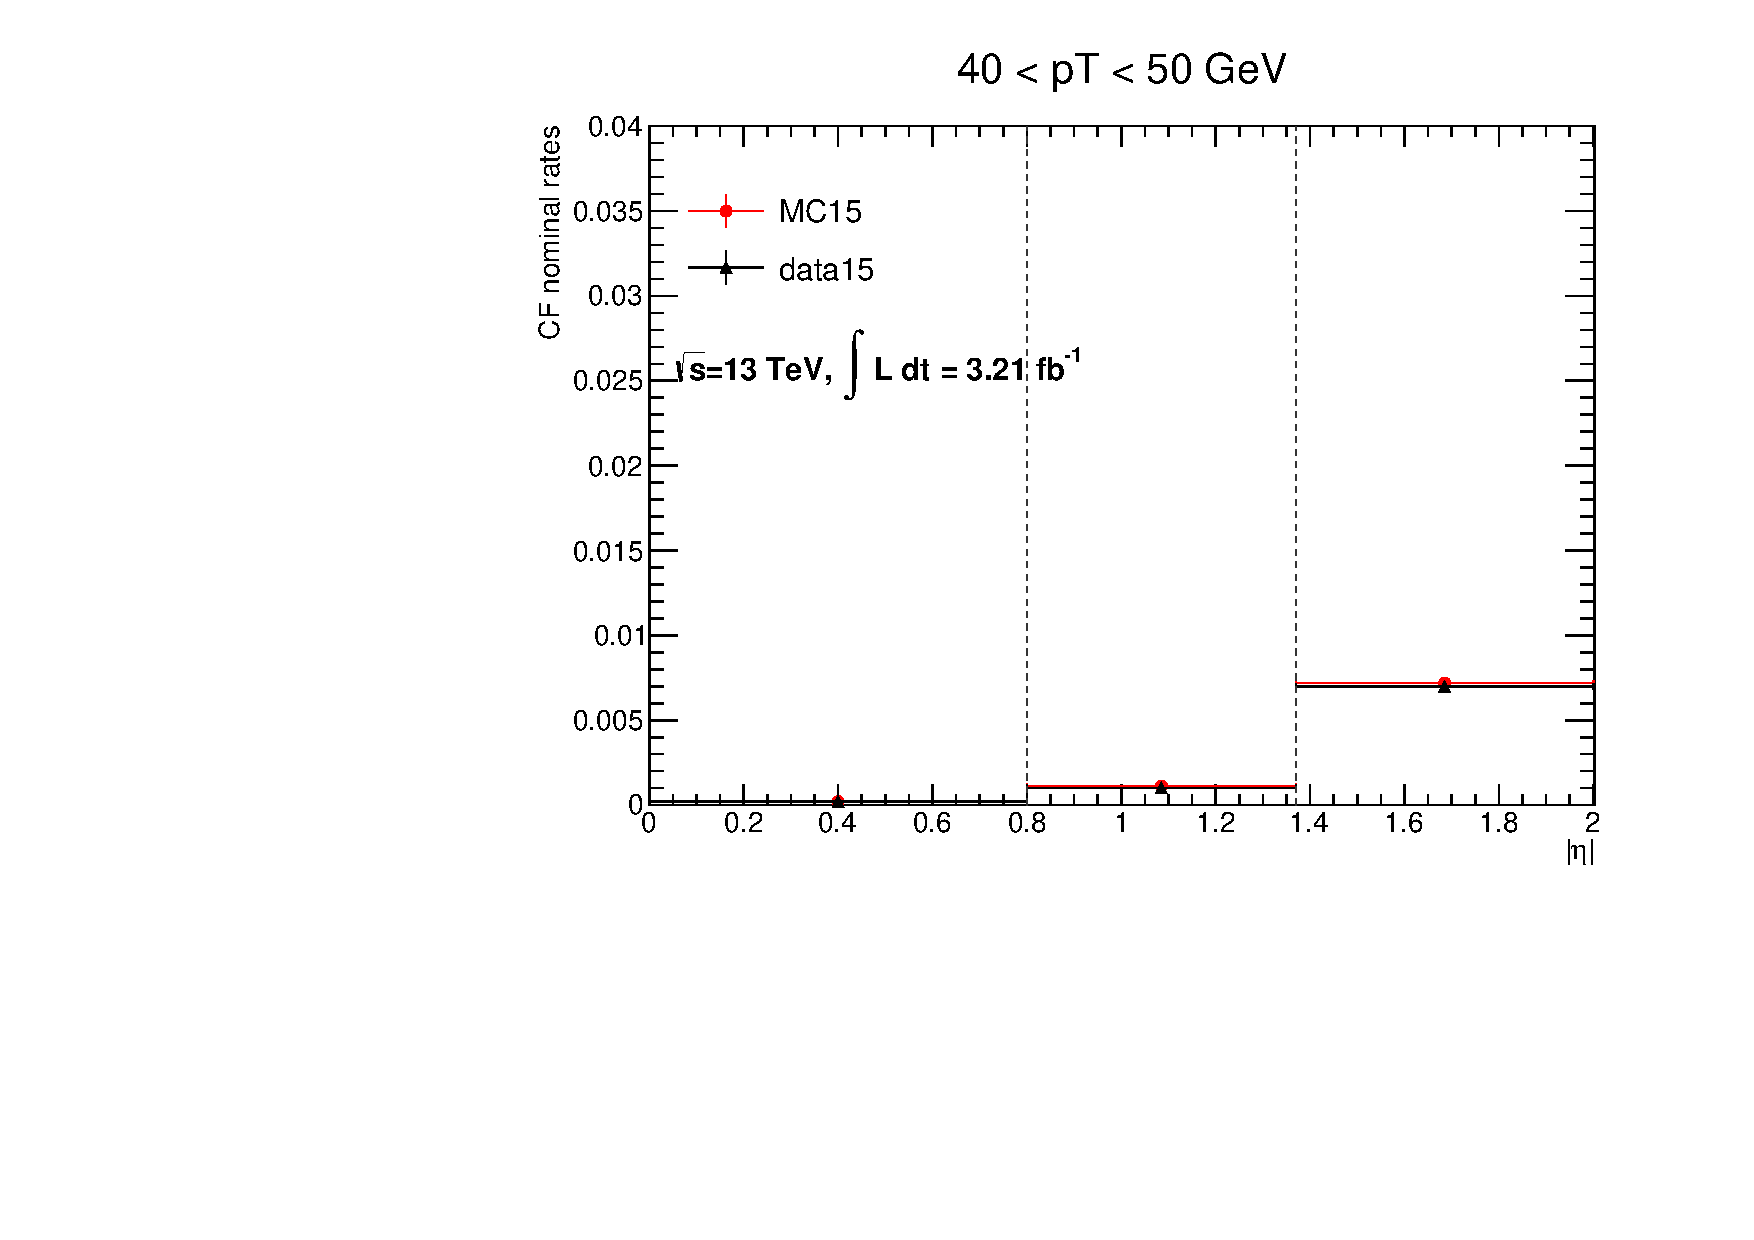
\includegraphics[width=0.4\textwidth]{FIGURES/BKG/chargeFlip/CFrates___dataVSmc___PTbin3.pdf}

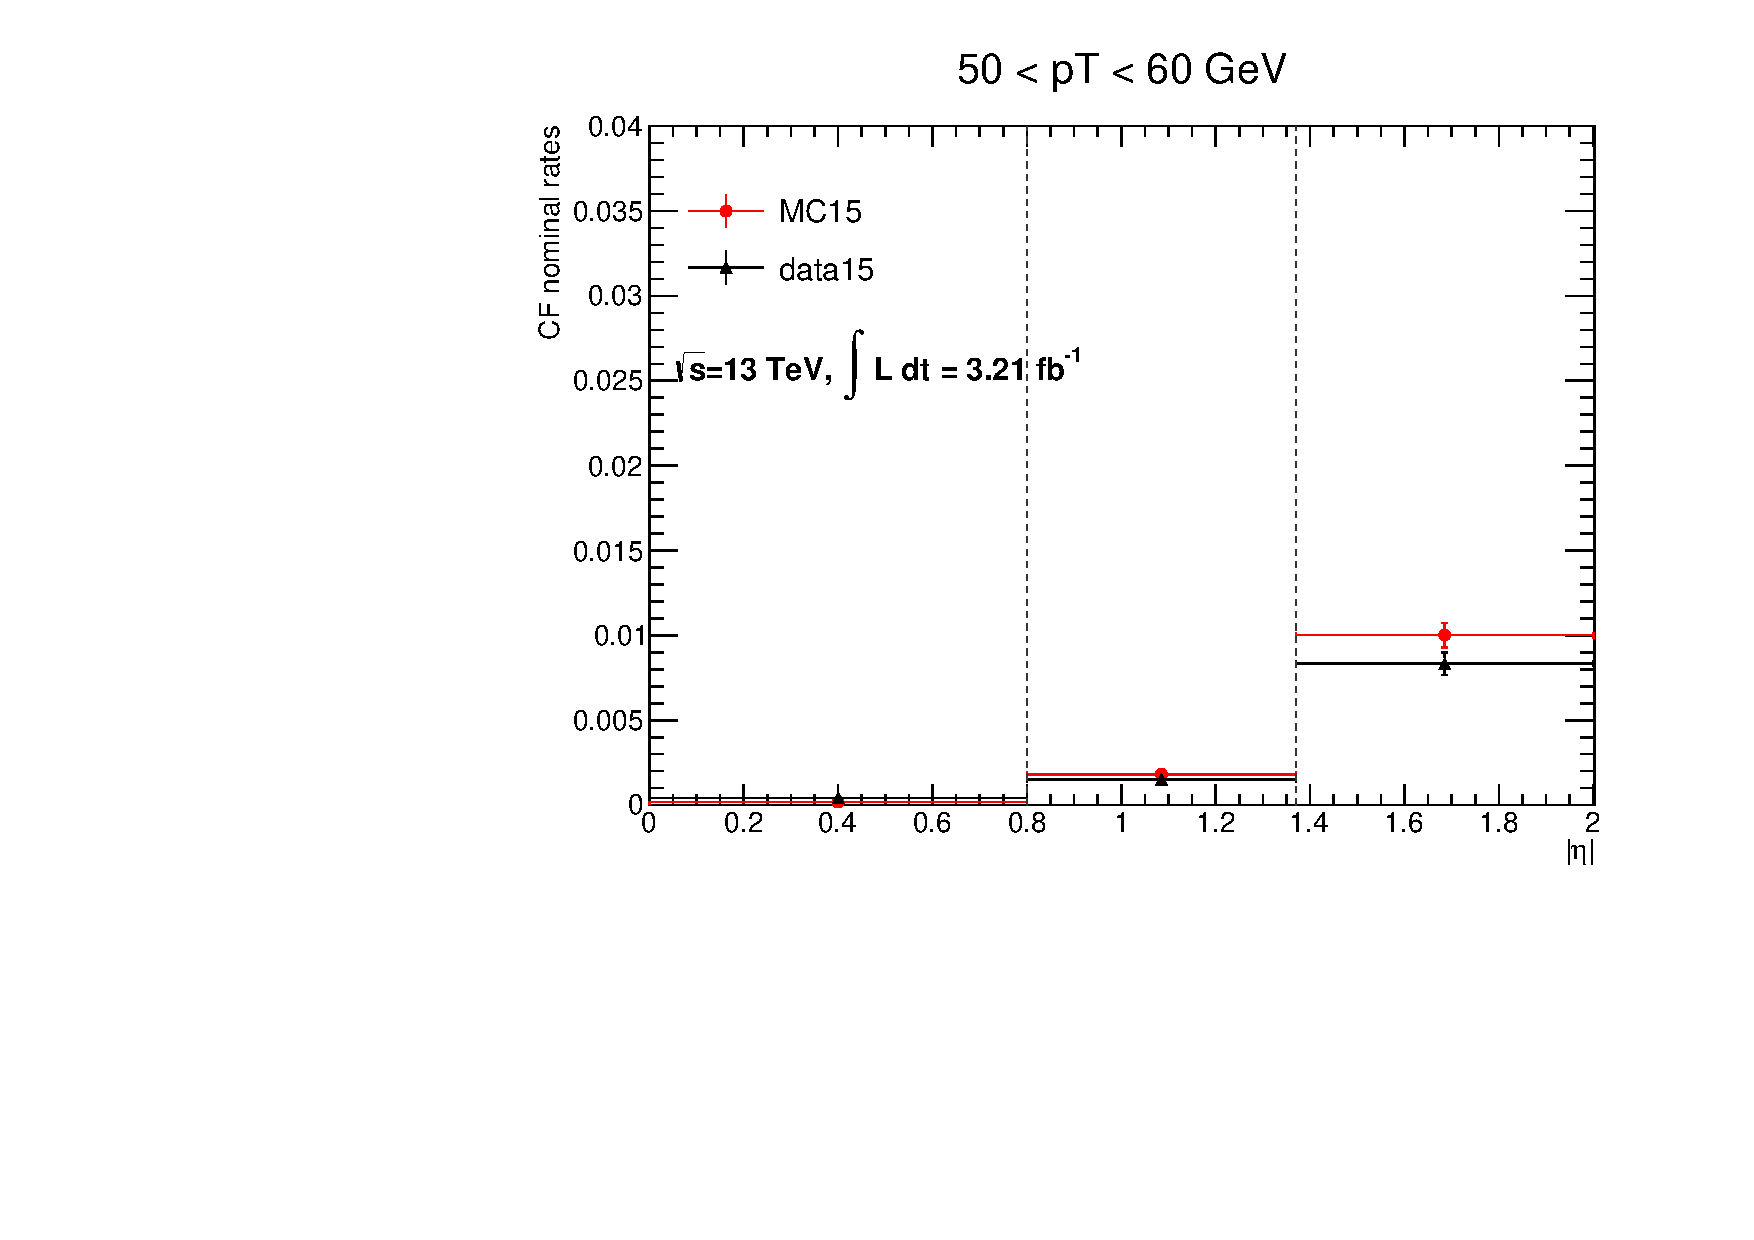
\includegraphics[width=0.4\textwidth]{FIGURES/BKG/chargeFlip/CFrates___dataVSmc___PTbin4.pdf}
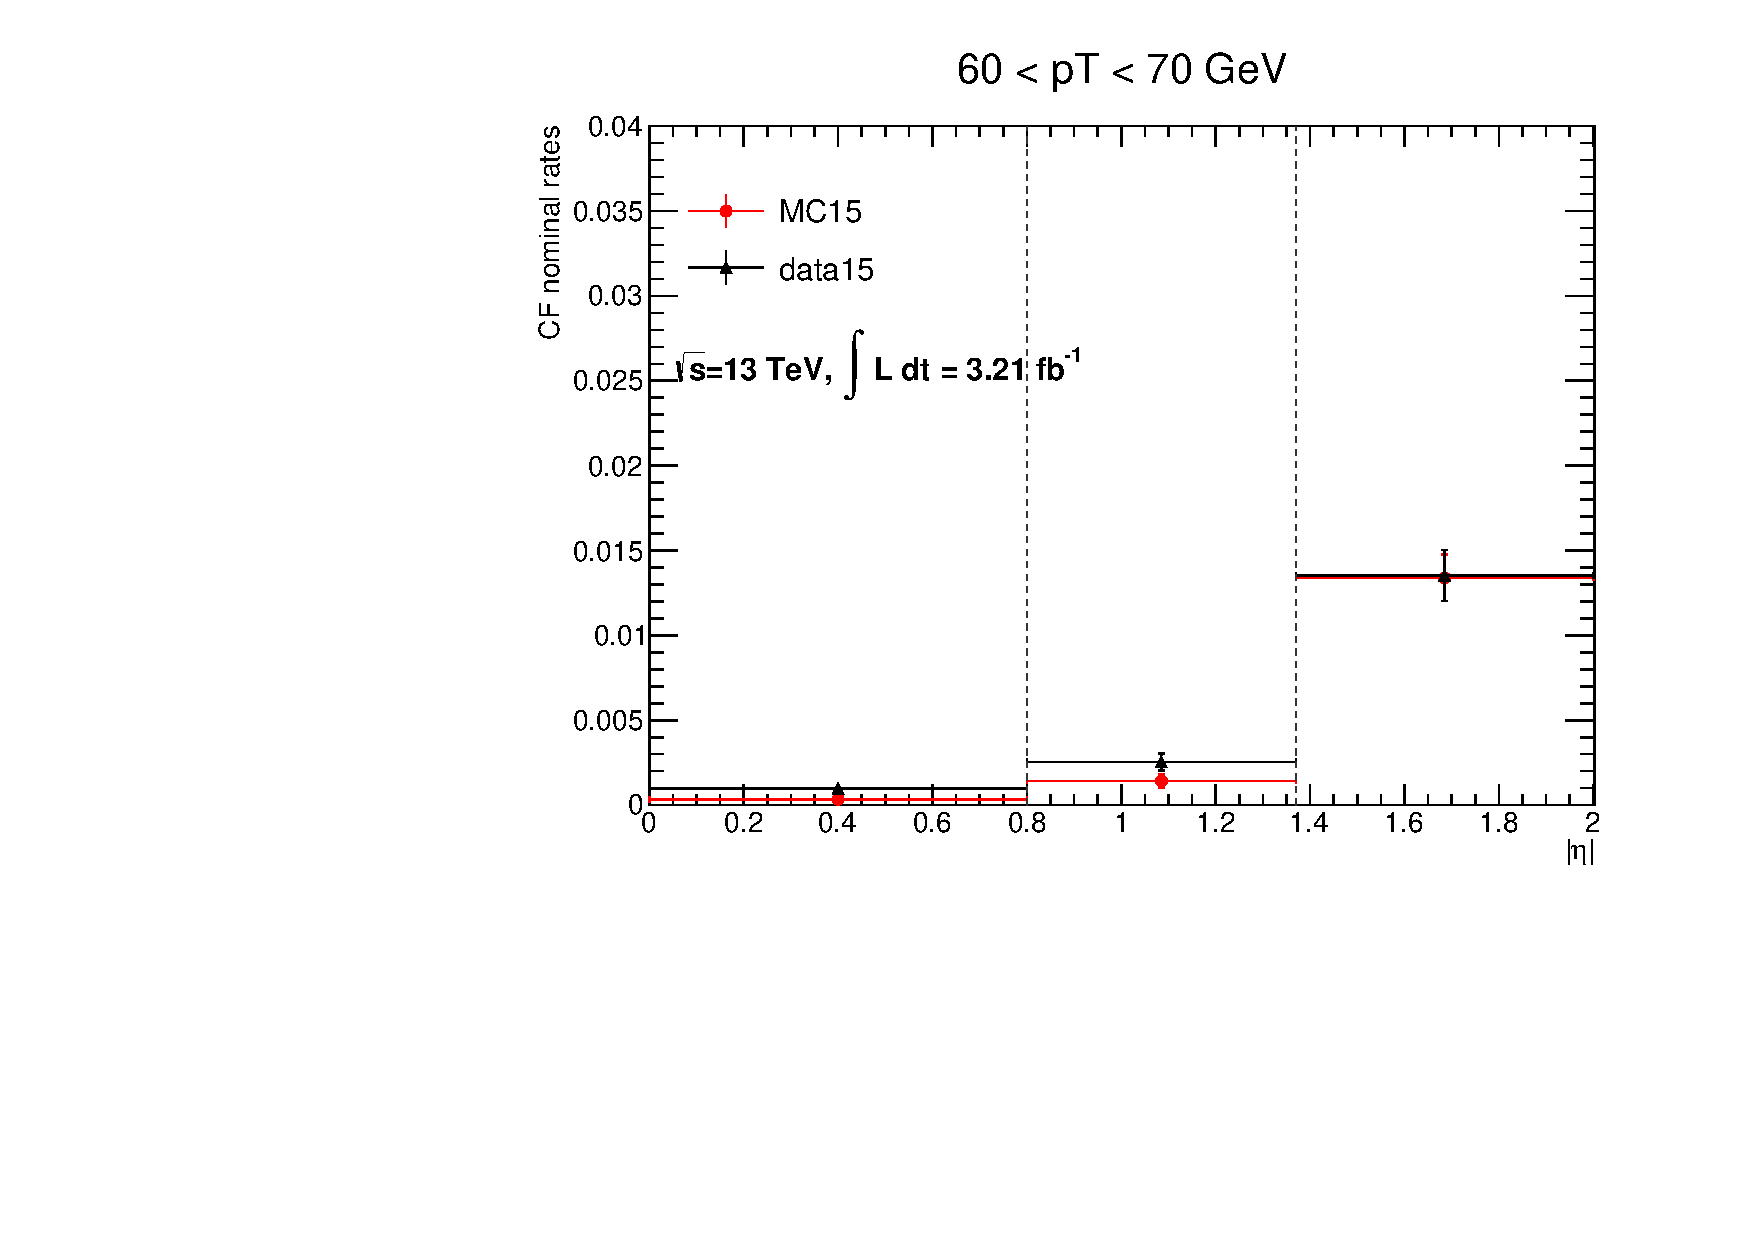
\includegraphics[width=0.4\textwidth]{FIGURES/BKG/chargeFlip/CFrates___dataVSmc___PTbin5.pdf}
\vfill
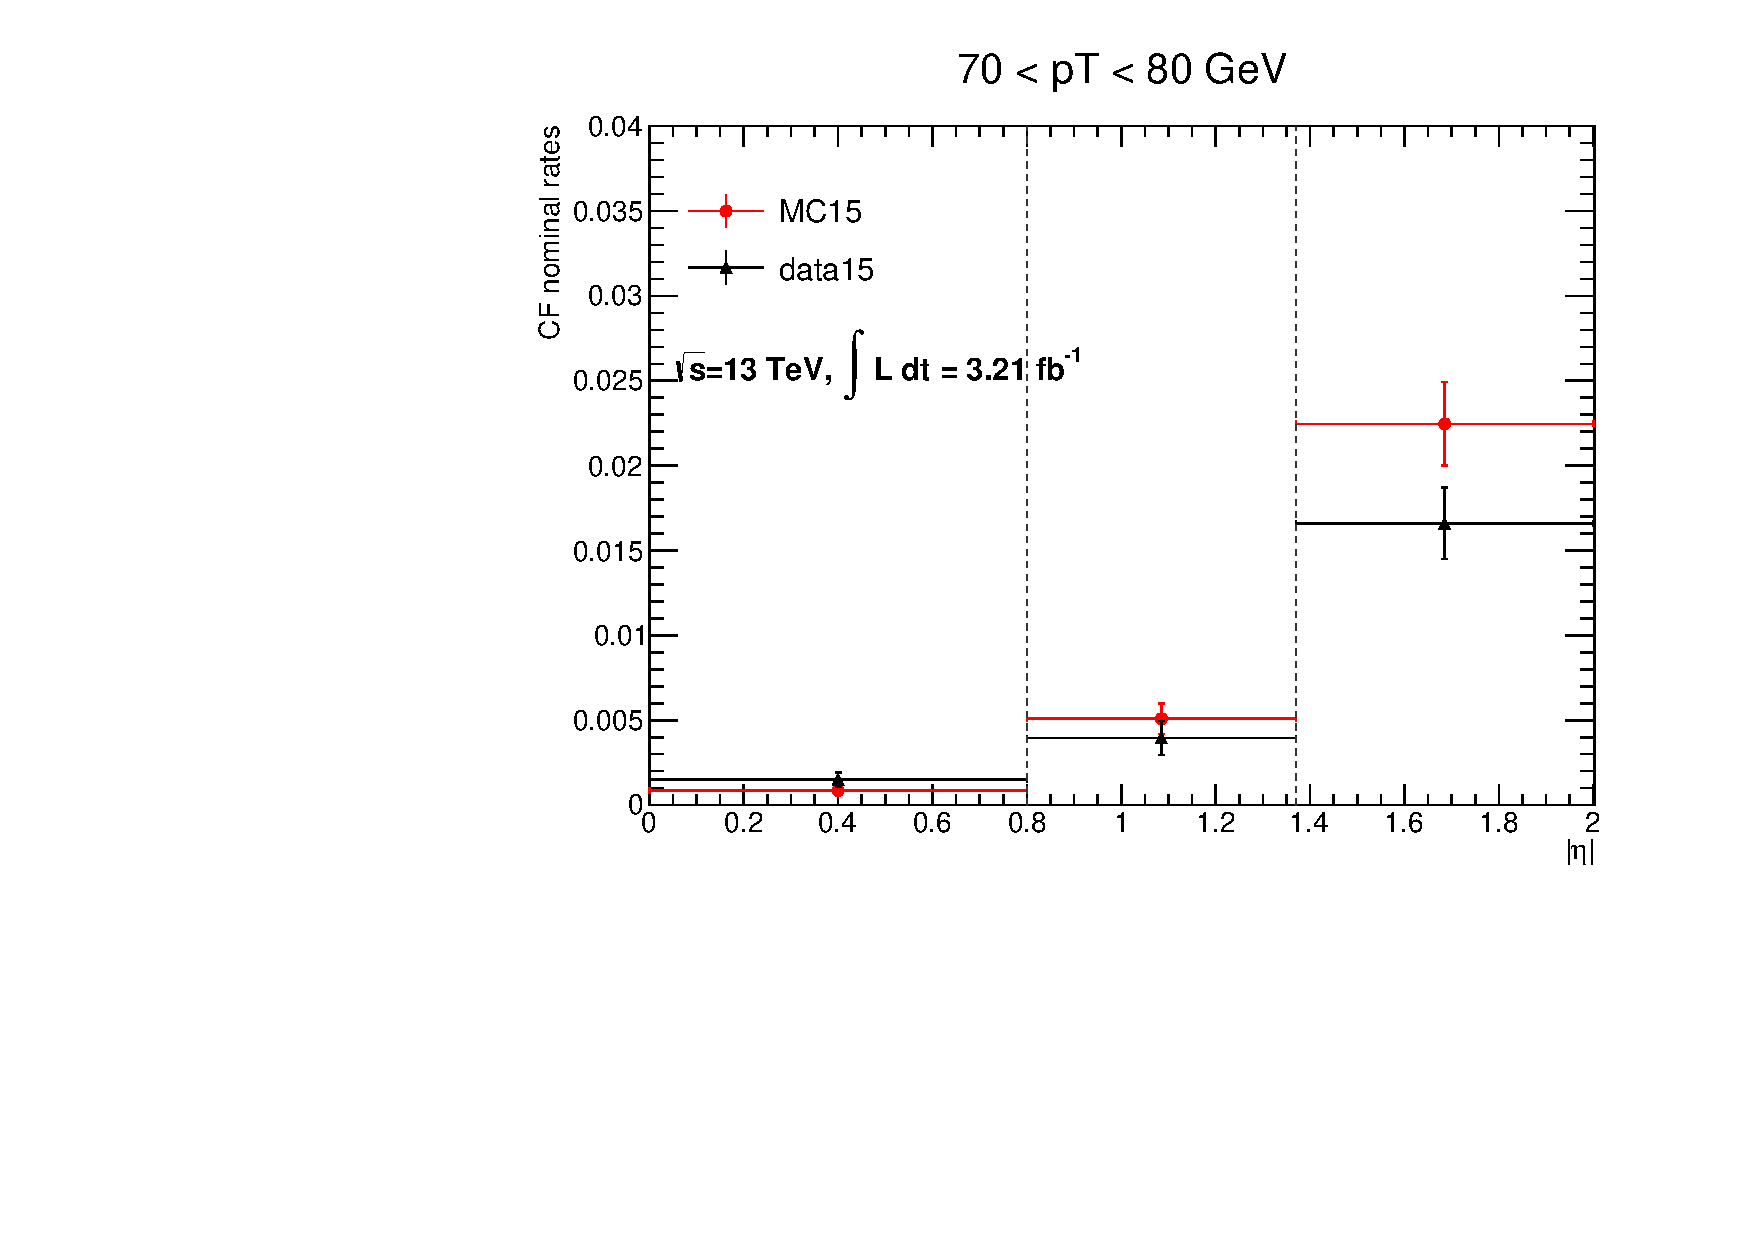
\includegraphics[width=0.4\textwidth]{FIGURES/BKG/chargeFlip/CFrates___dataVSmc___PTbin6.pdf}
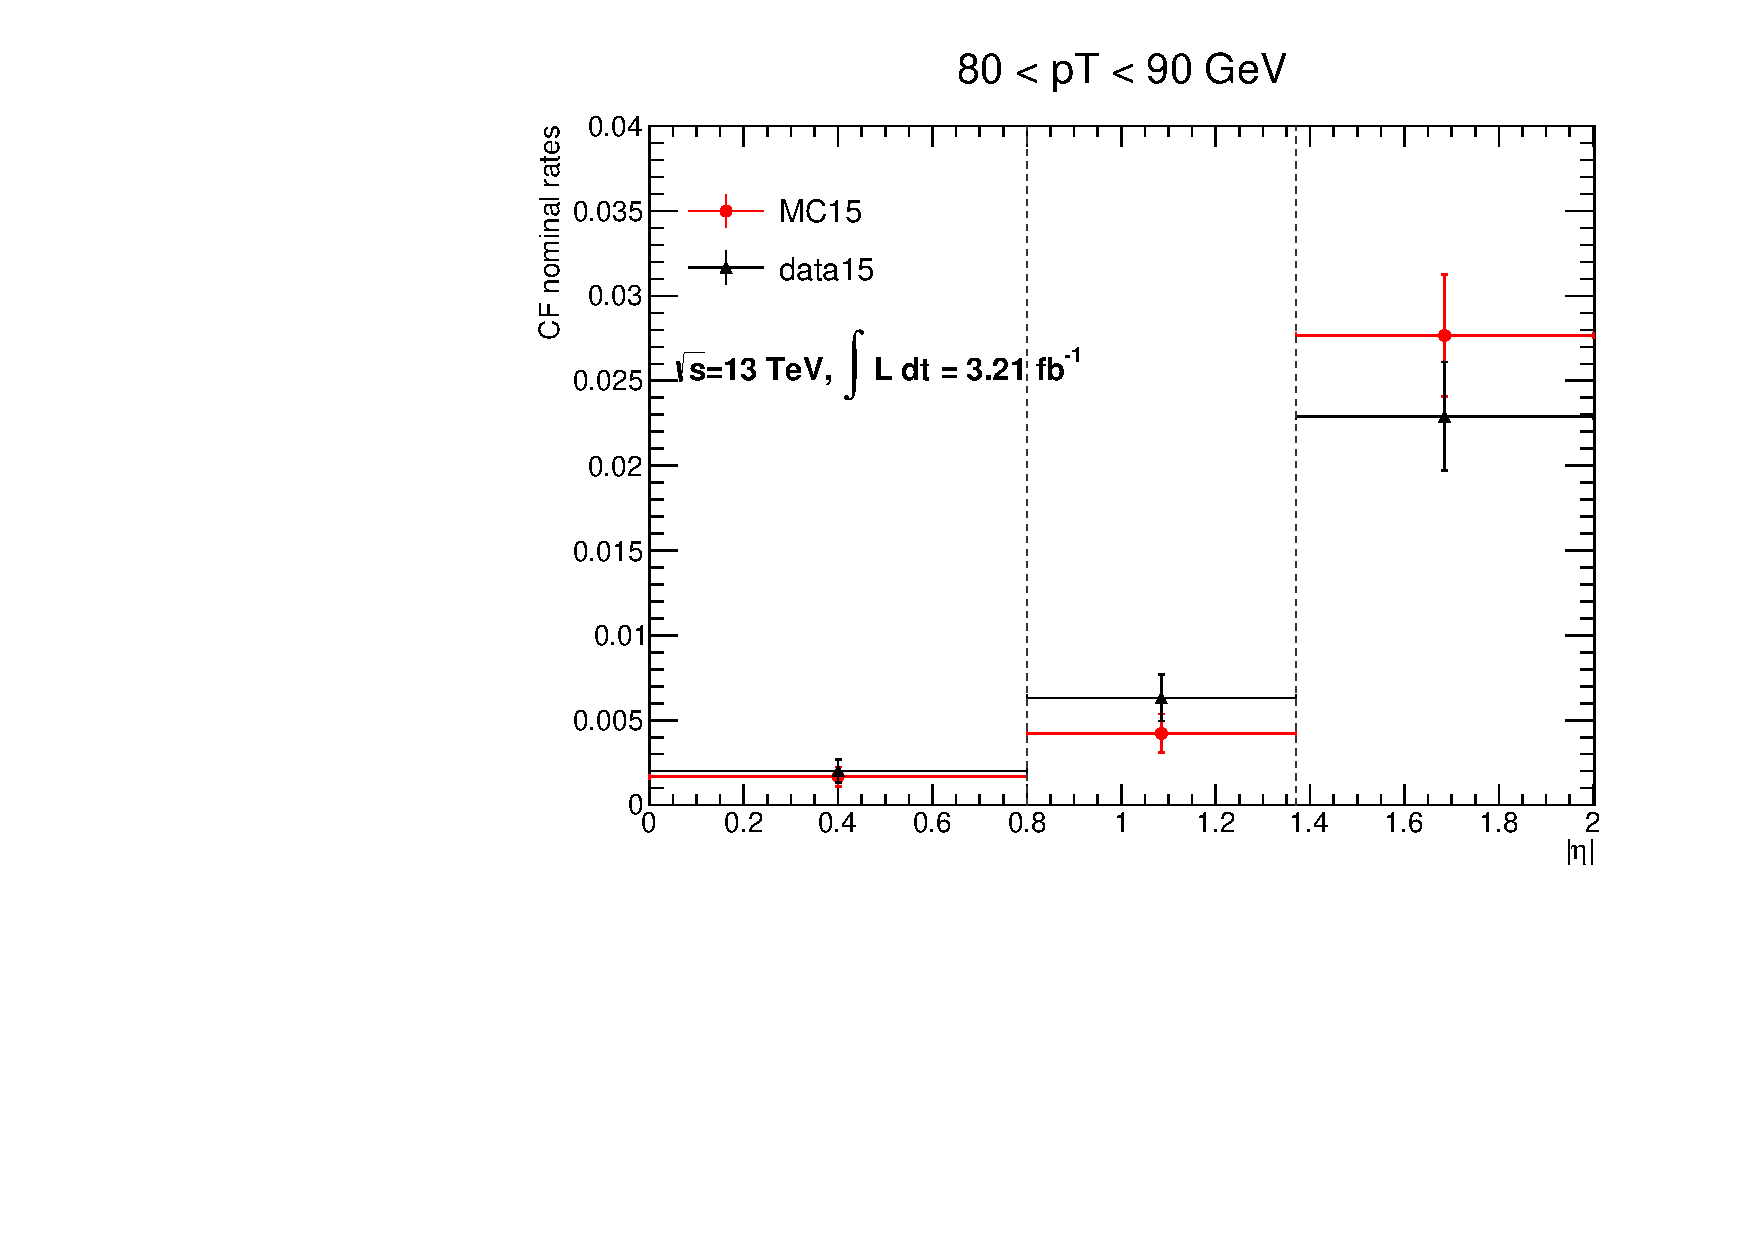
\includegraphics[width=0.4\textwidth]{FIGURES/BKG/chargeFlip/CFrates___dataVSmc___PTbin7.pdf}
\vfill
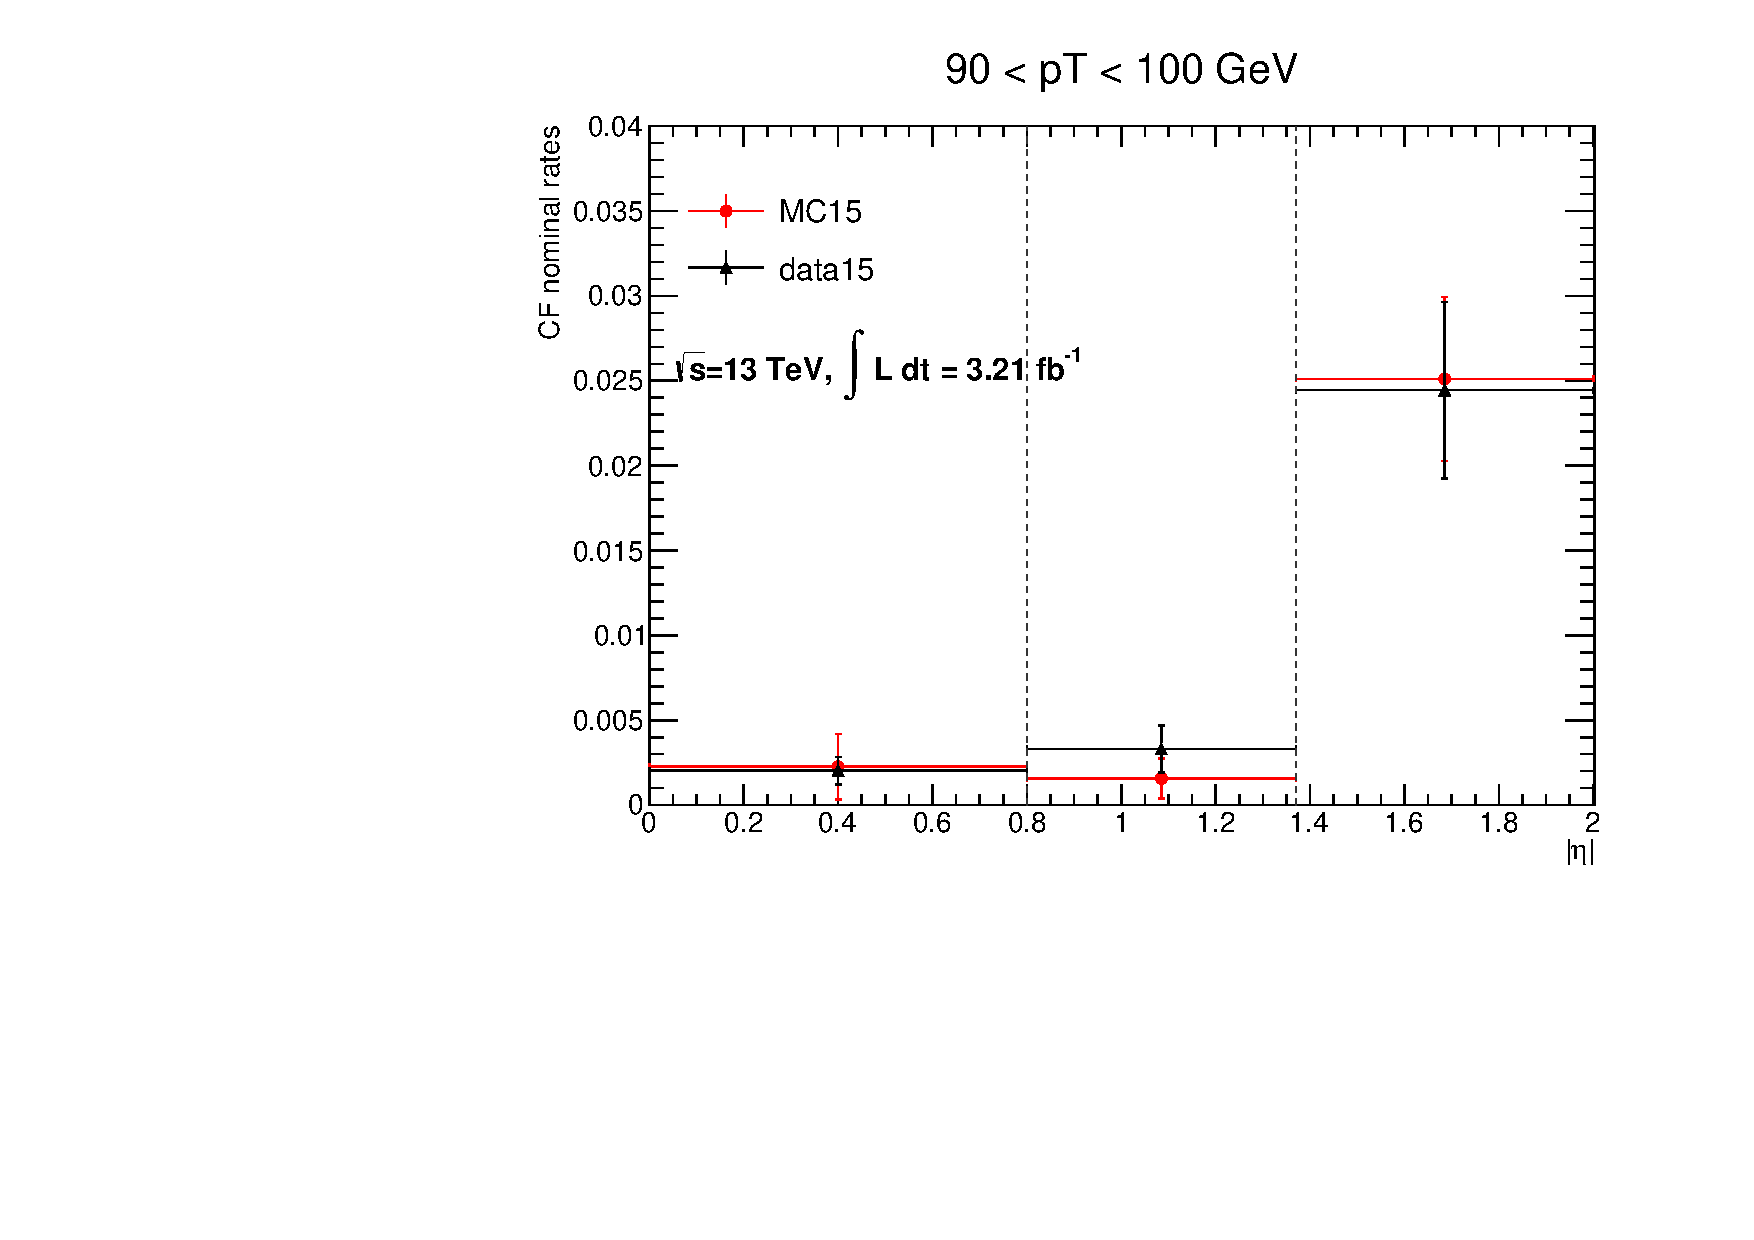
\includegraphics[width=0.4\textwidth]{FIGURES/BKG/chargeFlip/CFrates___dataVSmc___PTbin8.pdf}
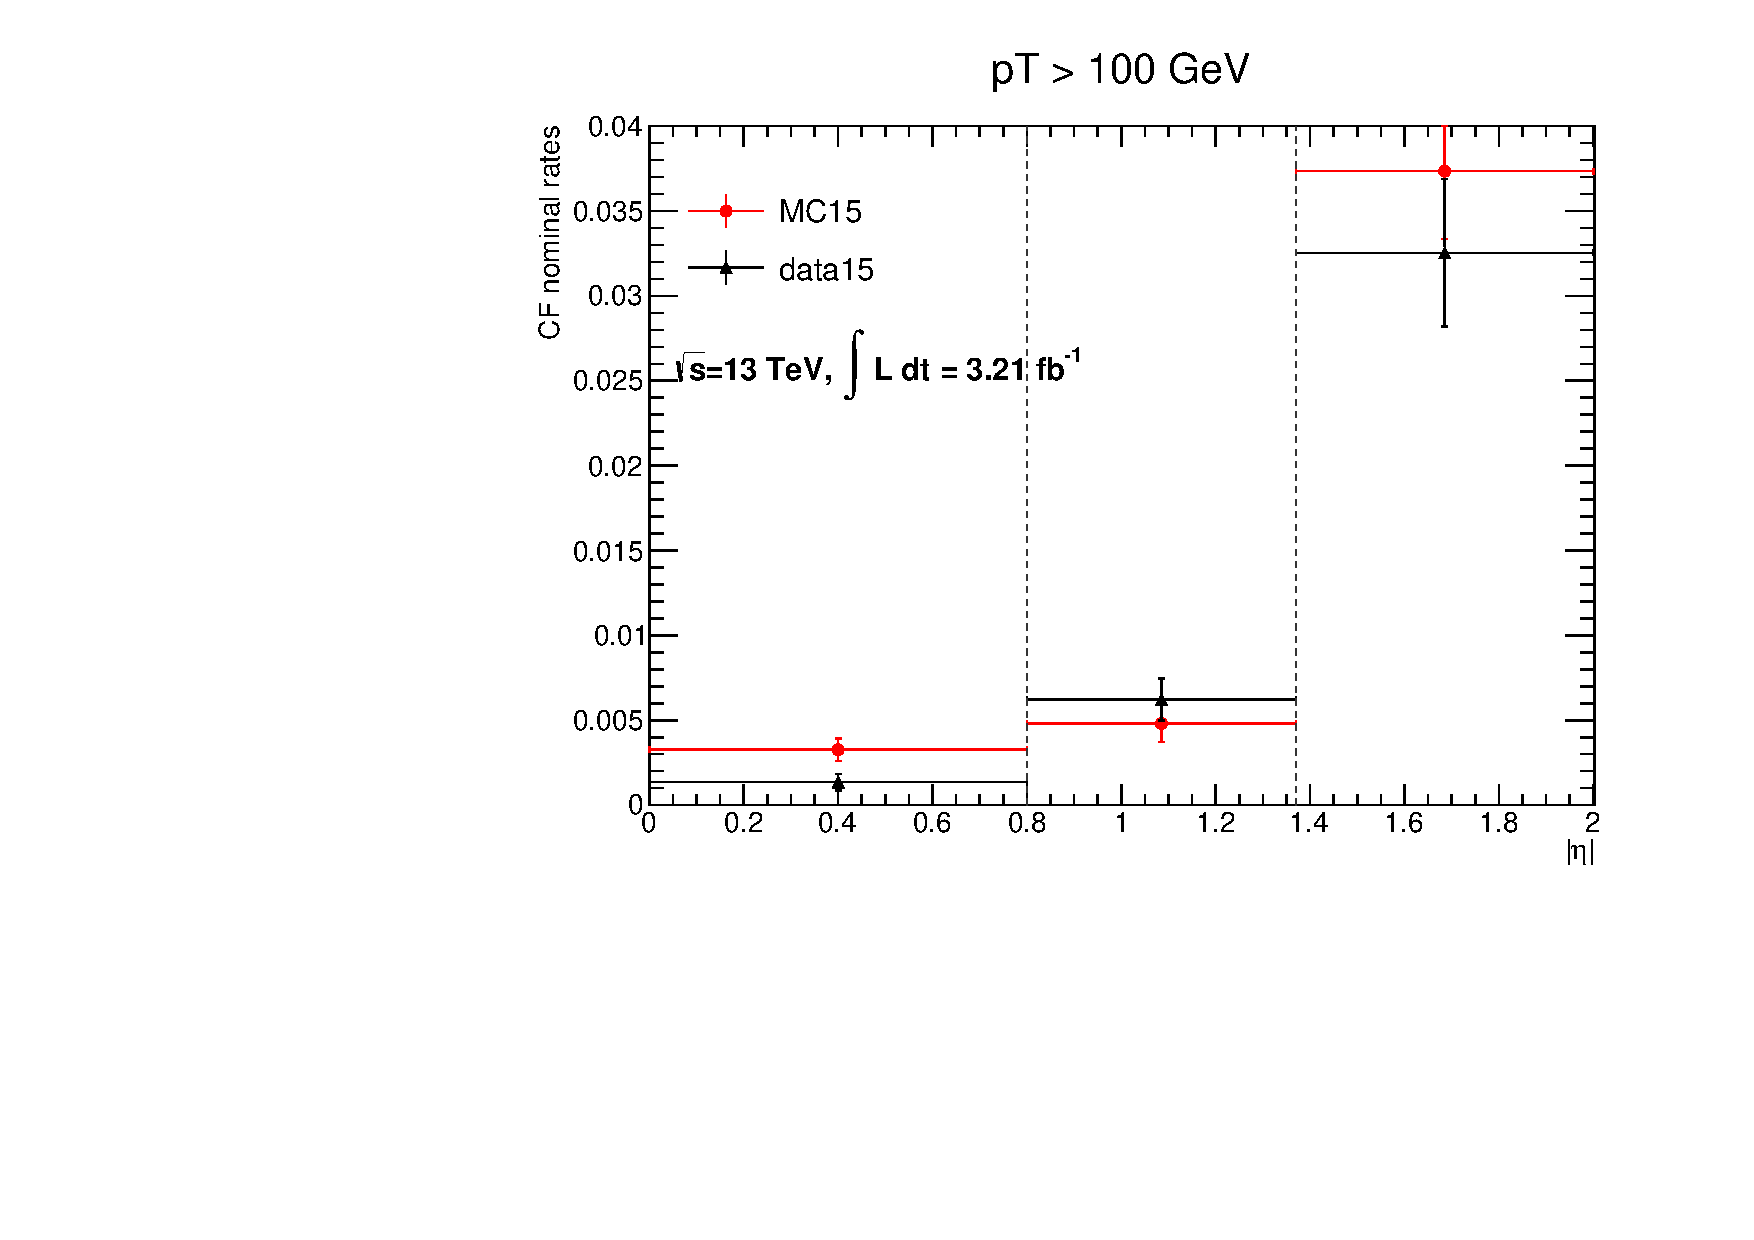
\includegraphics[width=0.4\textwidth]{FIGURES/BKG/chargeFlip/CFrates___dataVSmc___PTbin9.pdf}
\caption{\label{fig:CFratesNominal_1} Charge flip rates extracted from data (black dots) and from MC $Z\to e^+e^-$ (red dots) for electrons satisfying the signal requirements, as a function of $\eta$ and in various $\pt$ bins. Statistical and systematic uncertainties are shown.}
\end{figure}
%------------------------------------------------


%------------------------------------------------
\begin{figure}[h!]
\centering
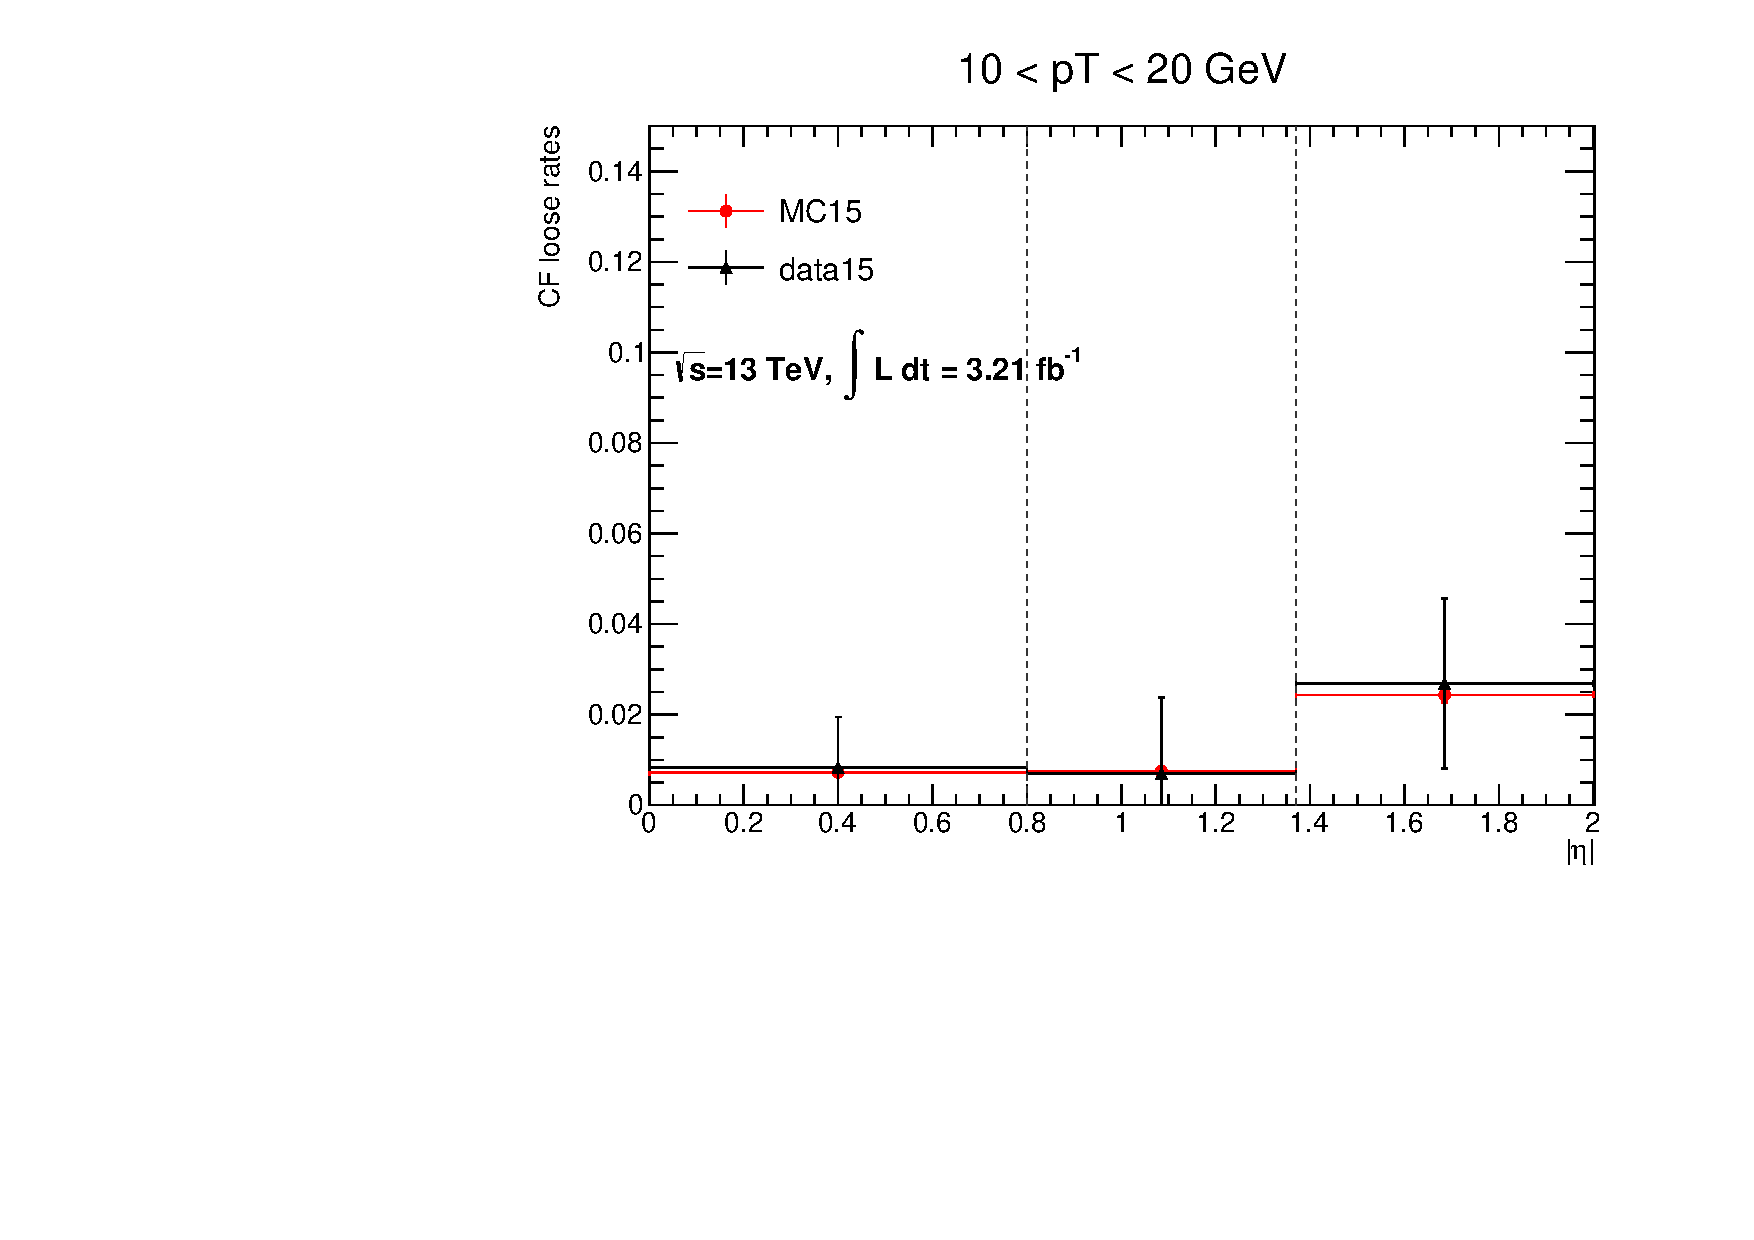
\includegraphics[width=0.4\textwidth]{FIGURES/BKG/chargeFlip/CFratesLOOSE___dataVSmc___PTbin0.pdf}
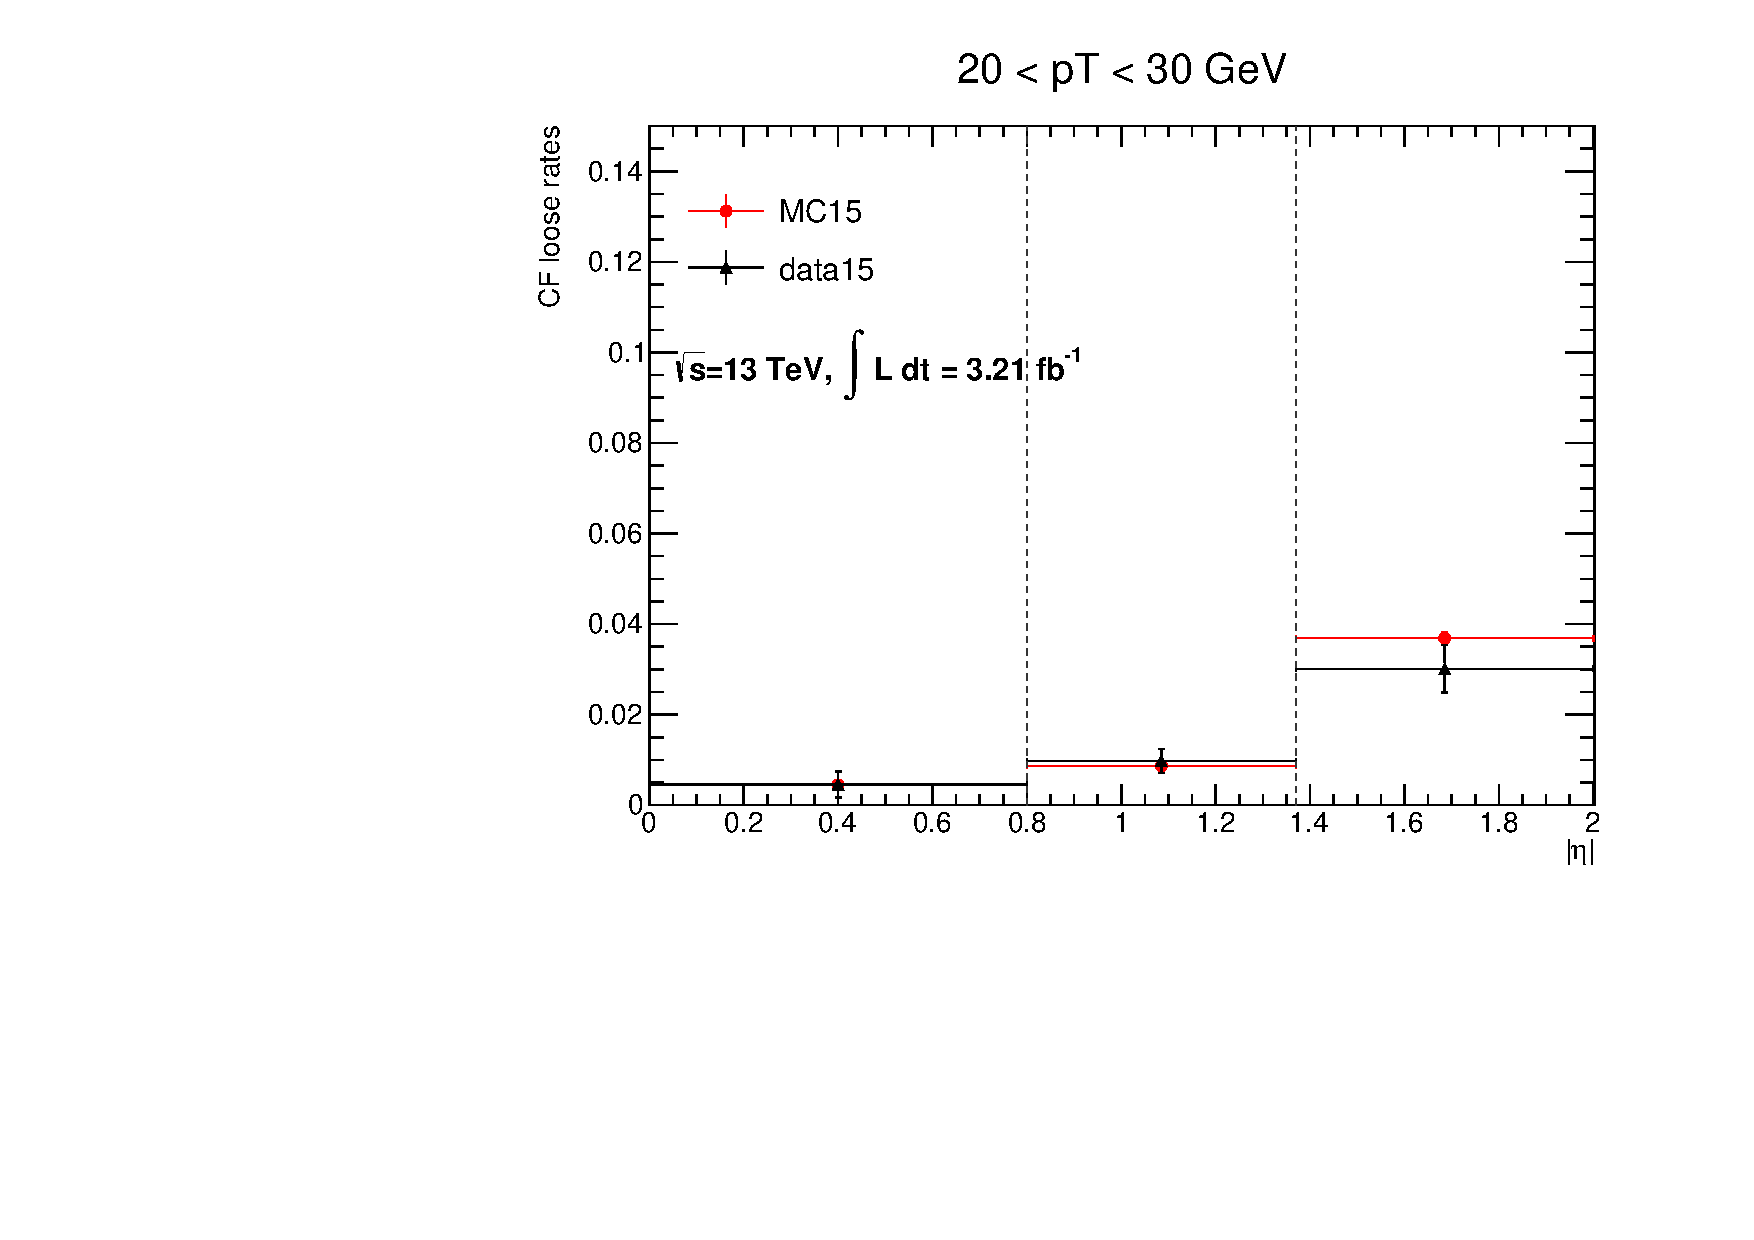
\includegraphics[width=0.4\textwidth]{FIGURES/BKG/chargeFlip/CFratesLOOSE___dataVSmc___PTbin1.pdf}
\vfill
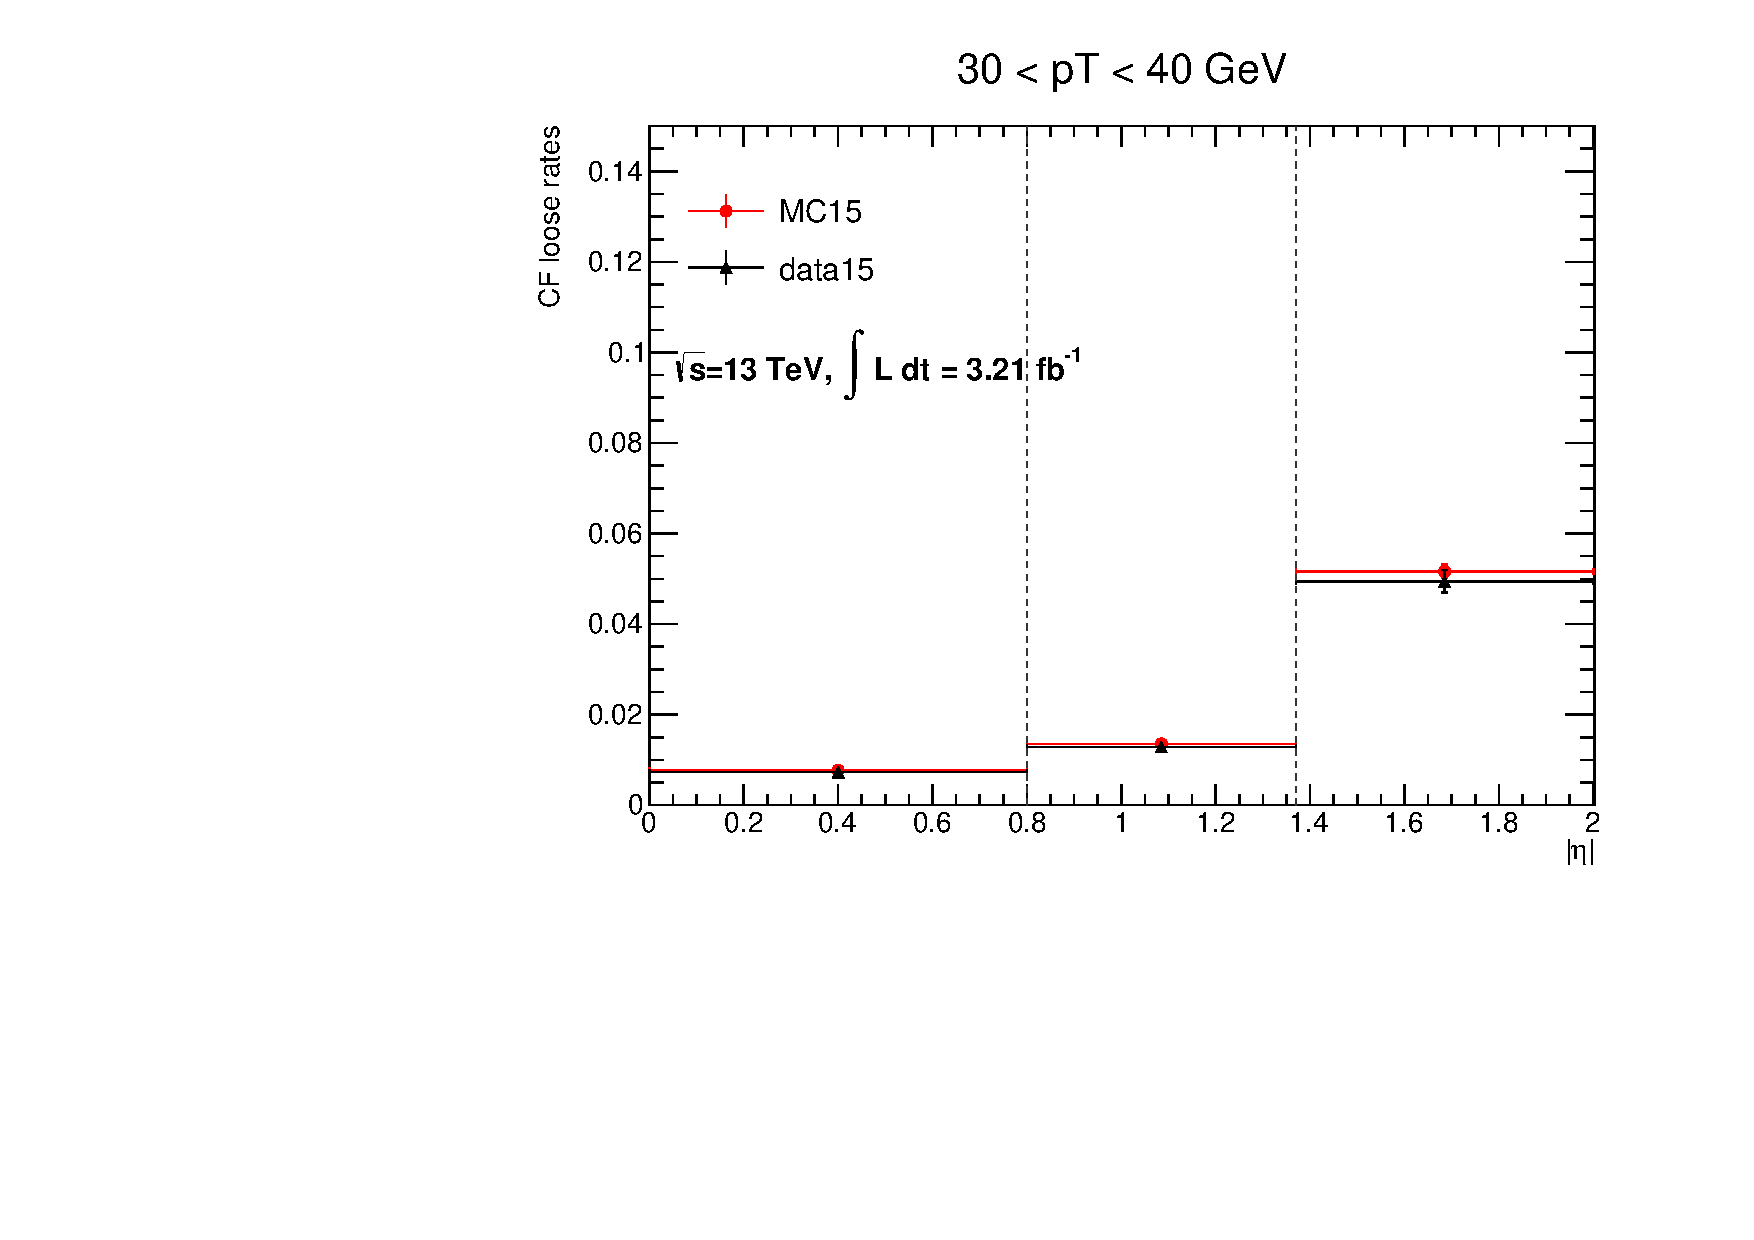
\includegraphics[width=0.4\textwidth]{FIGURES/BKG/chargeFlip/CFratesLOOSE___dataVSmc___PTbin2.pdf}
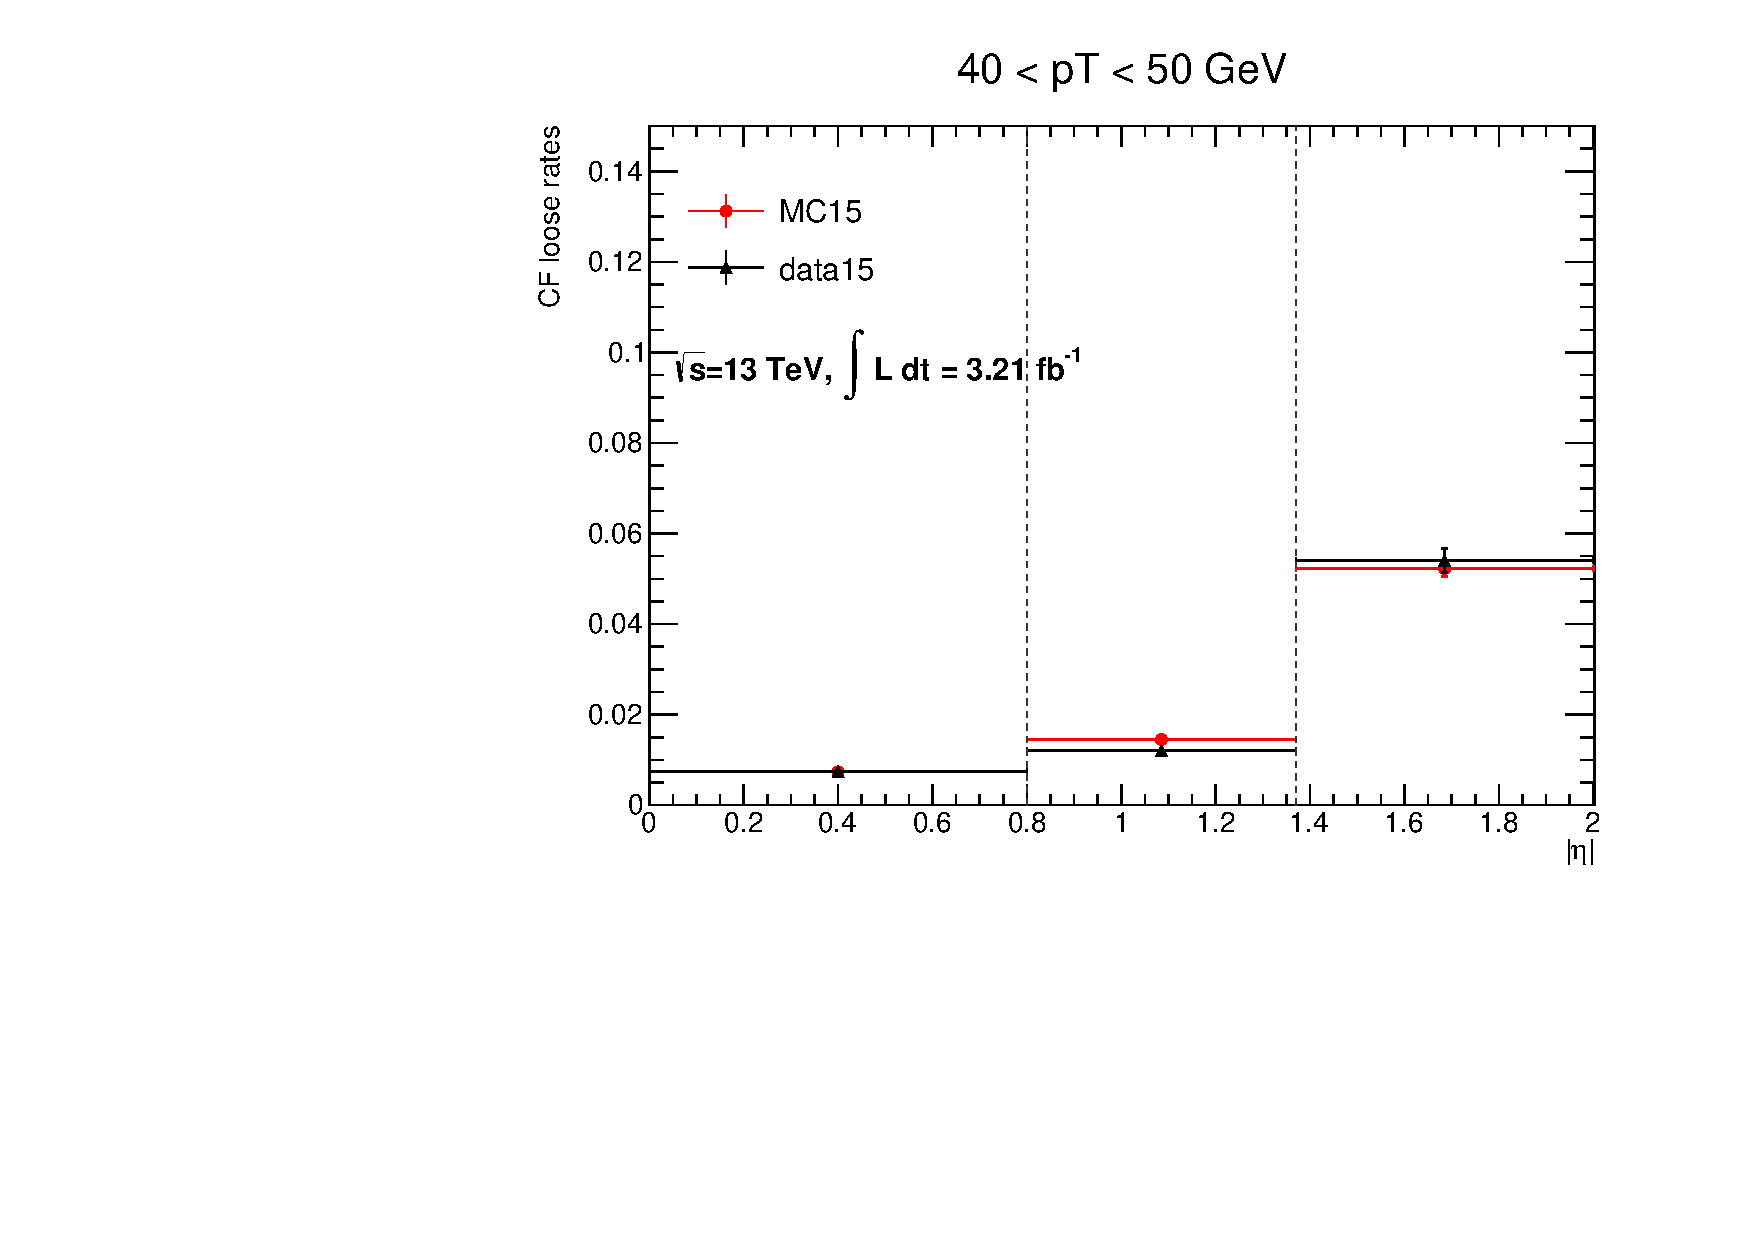
\includegraphics[width=0.4\textwidth]{FIGURES/BKG/chargeFlip/CFratesLOOSE___dataVSmc___PTbin3.pdf}

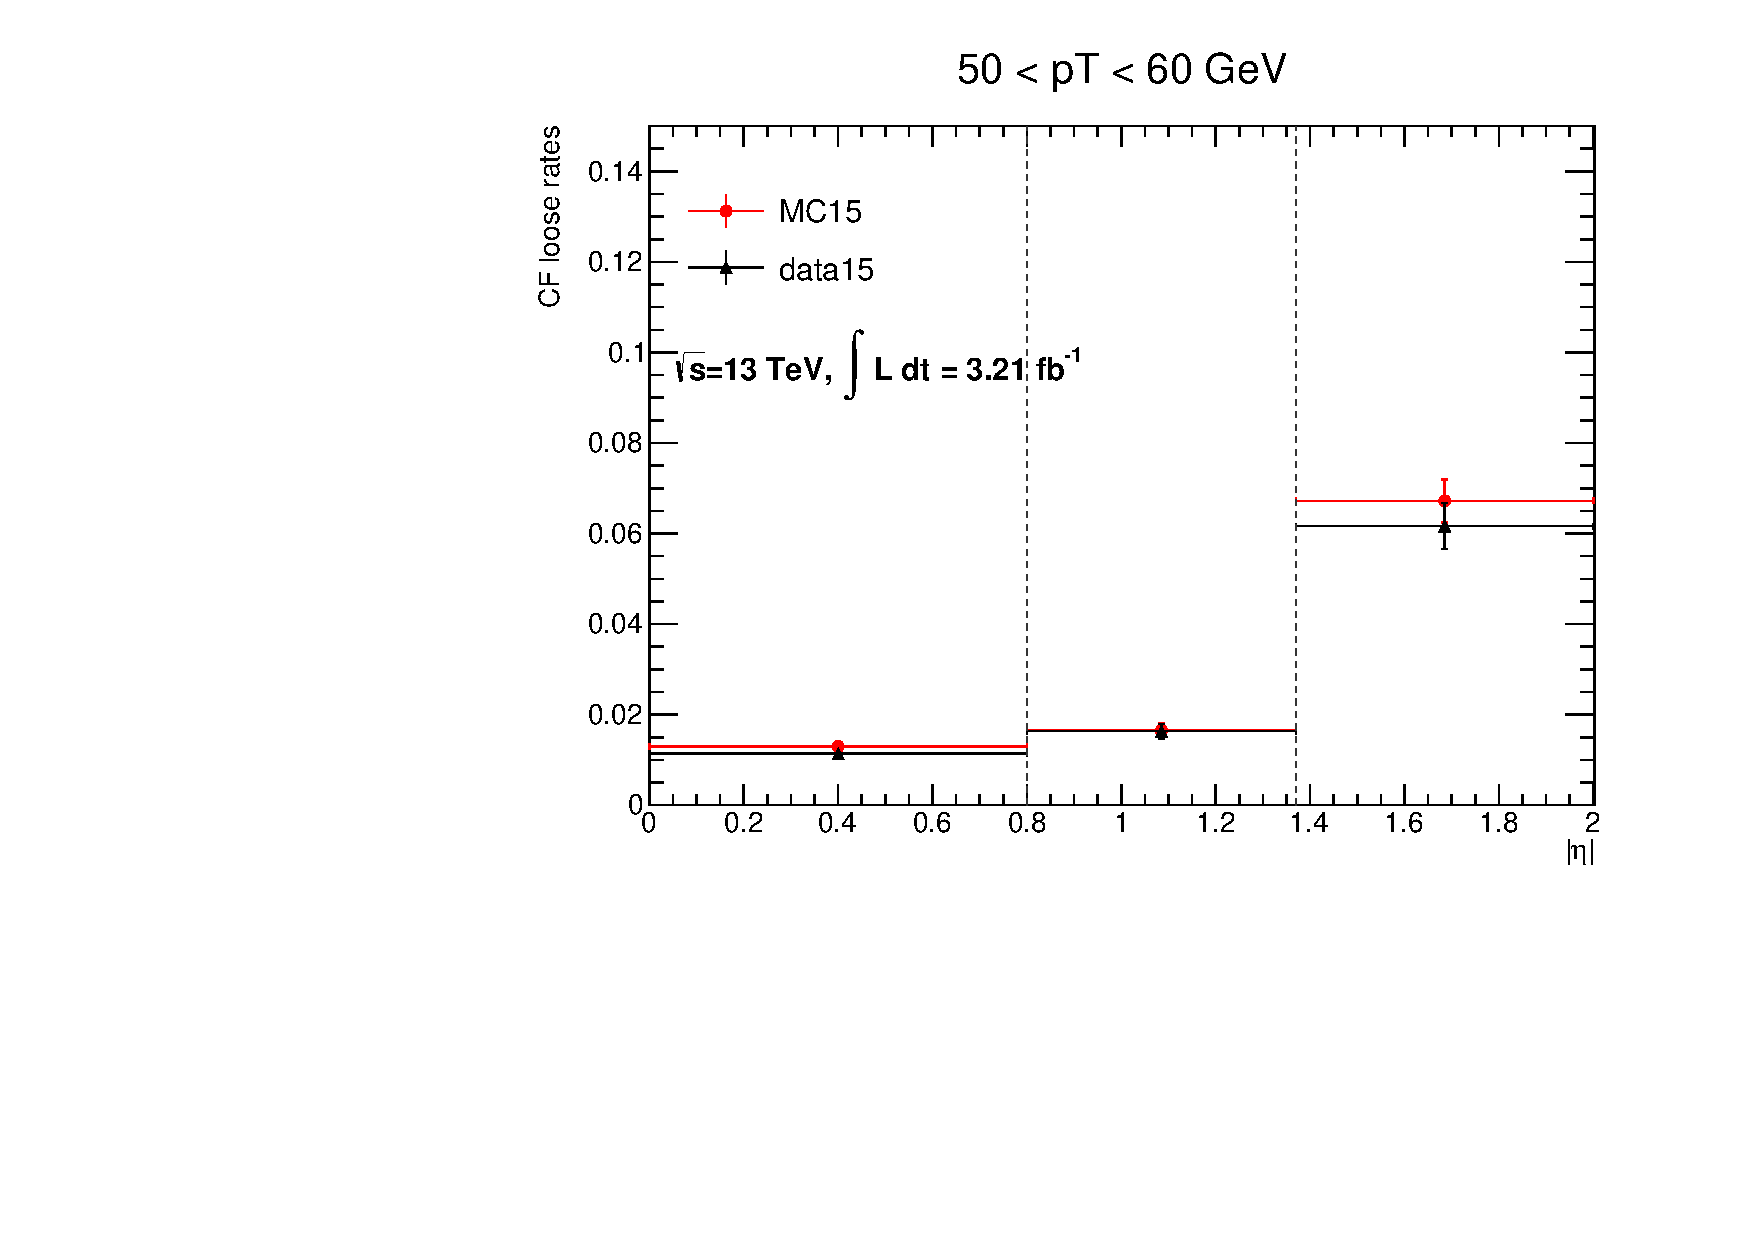
\includegraphics[width=0.4\textwidth]{FIGURES/BKG/chargeFlip/CFratesLOOSE___dataVSmc___PTbin4.pdf}
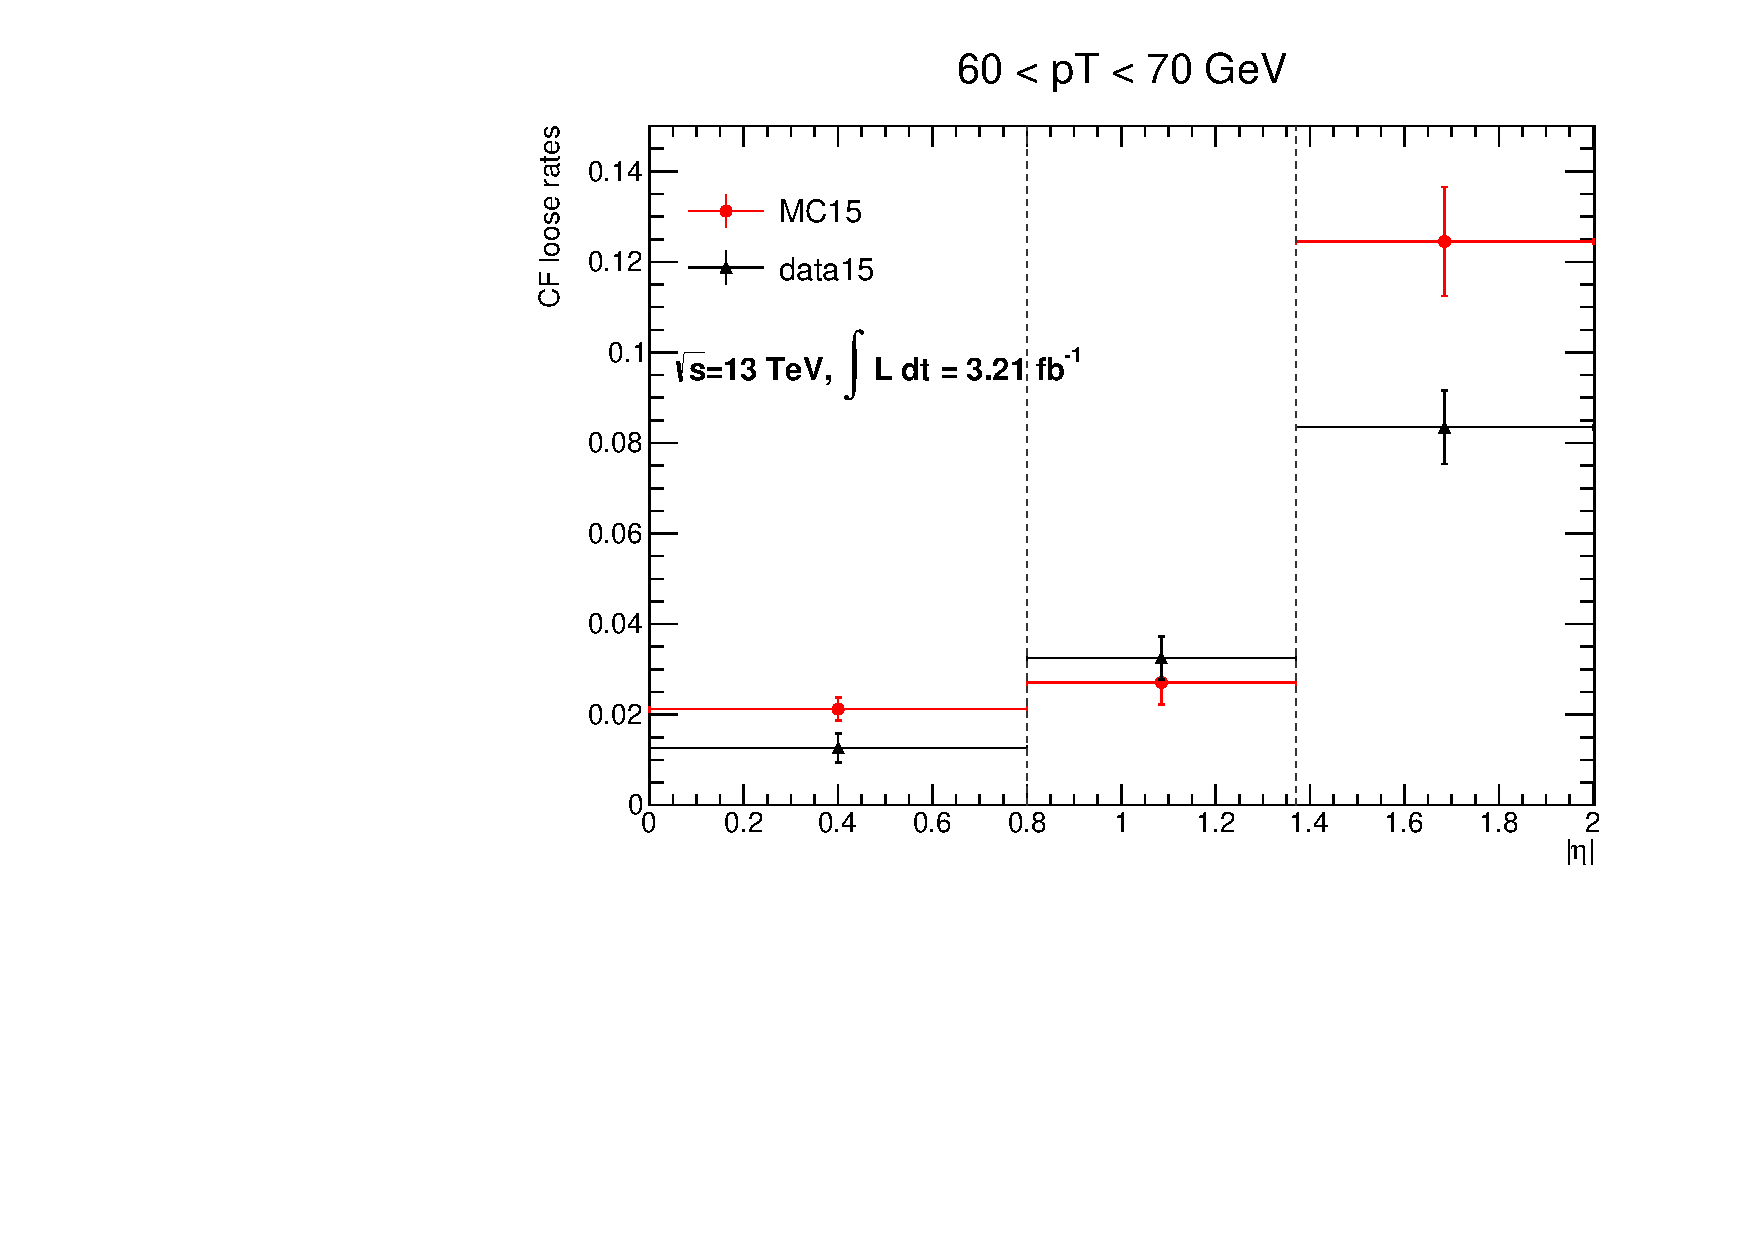
\includegraphics[width=0.4\textwidth]{FIGURES/BKG/chargeFlip/CFratesLOOSE___dataVSmc___PTbin5.pdf}
\vfill
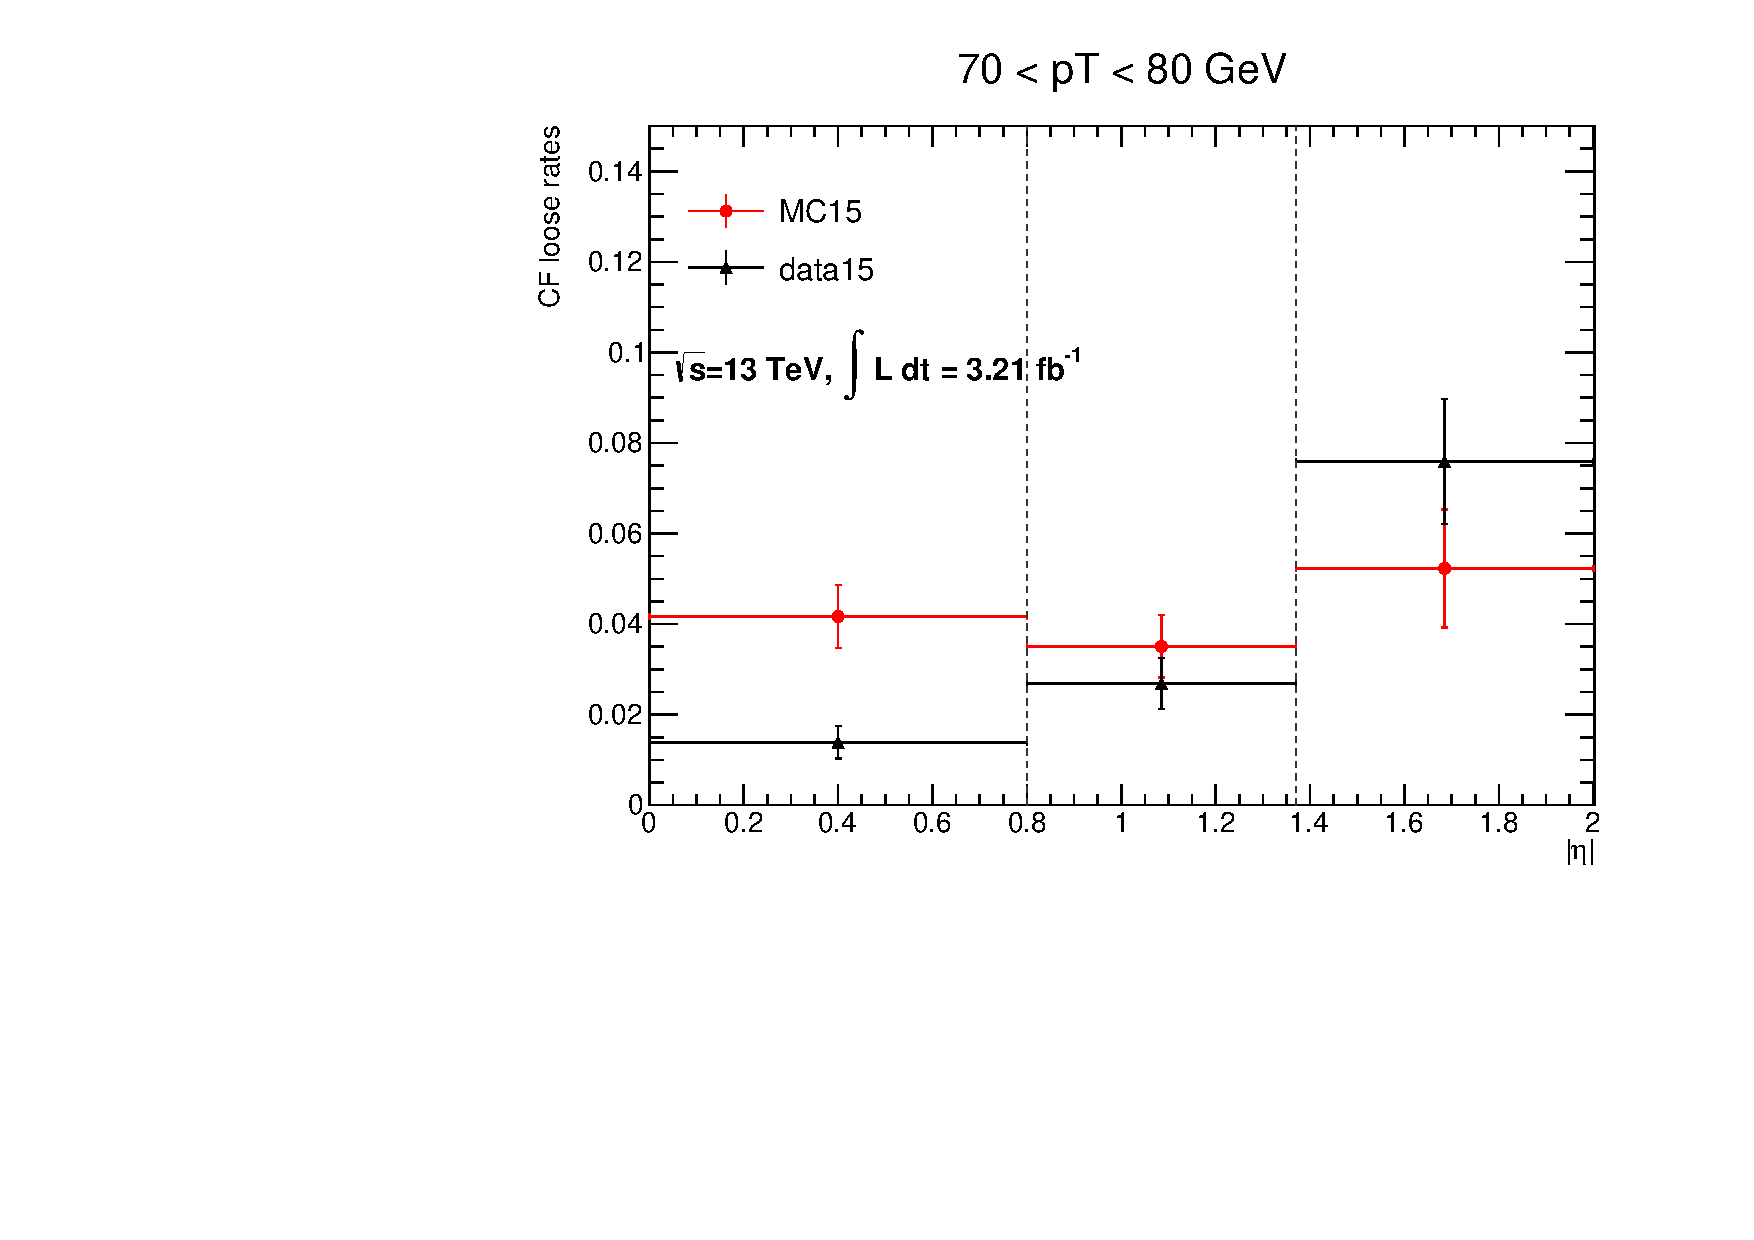
\includegraphics[width=0.4\textwidth]{FIGURES/BKG/chargeFlip/CFratesLOOSE___dataVSmc___PTbin6.pdf}
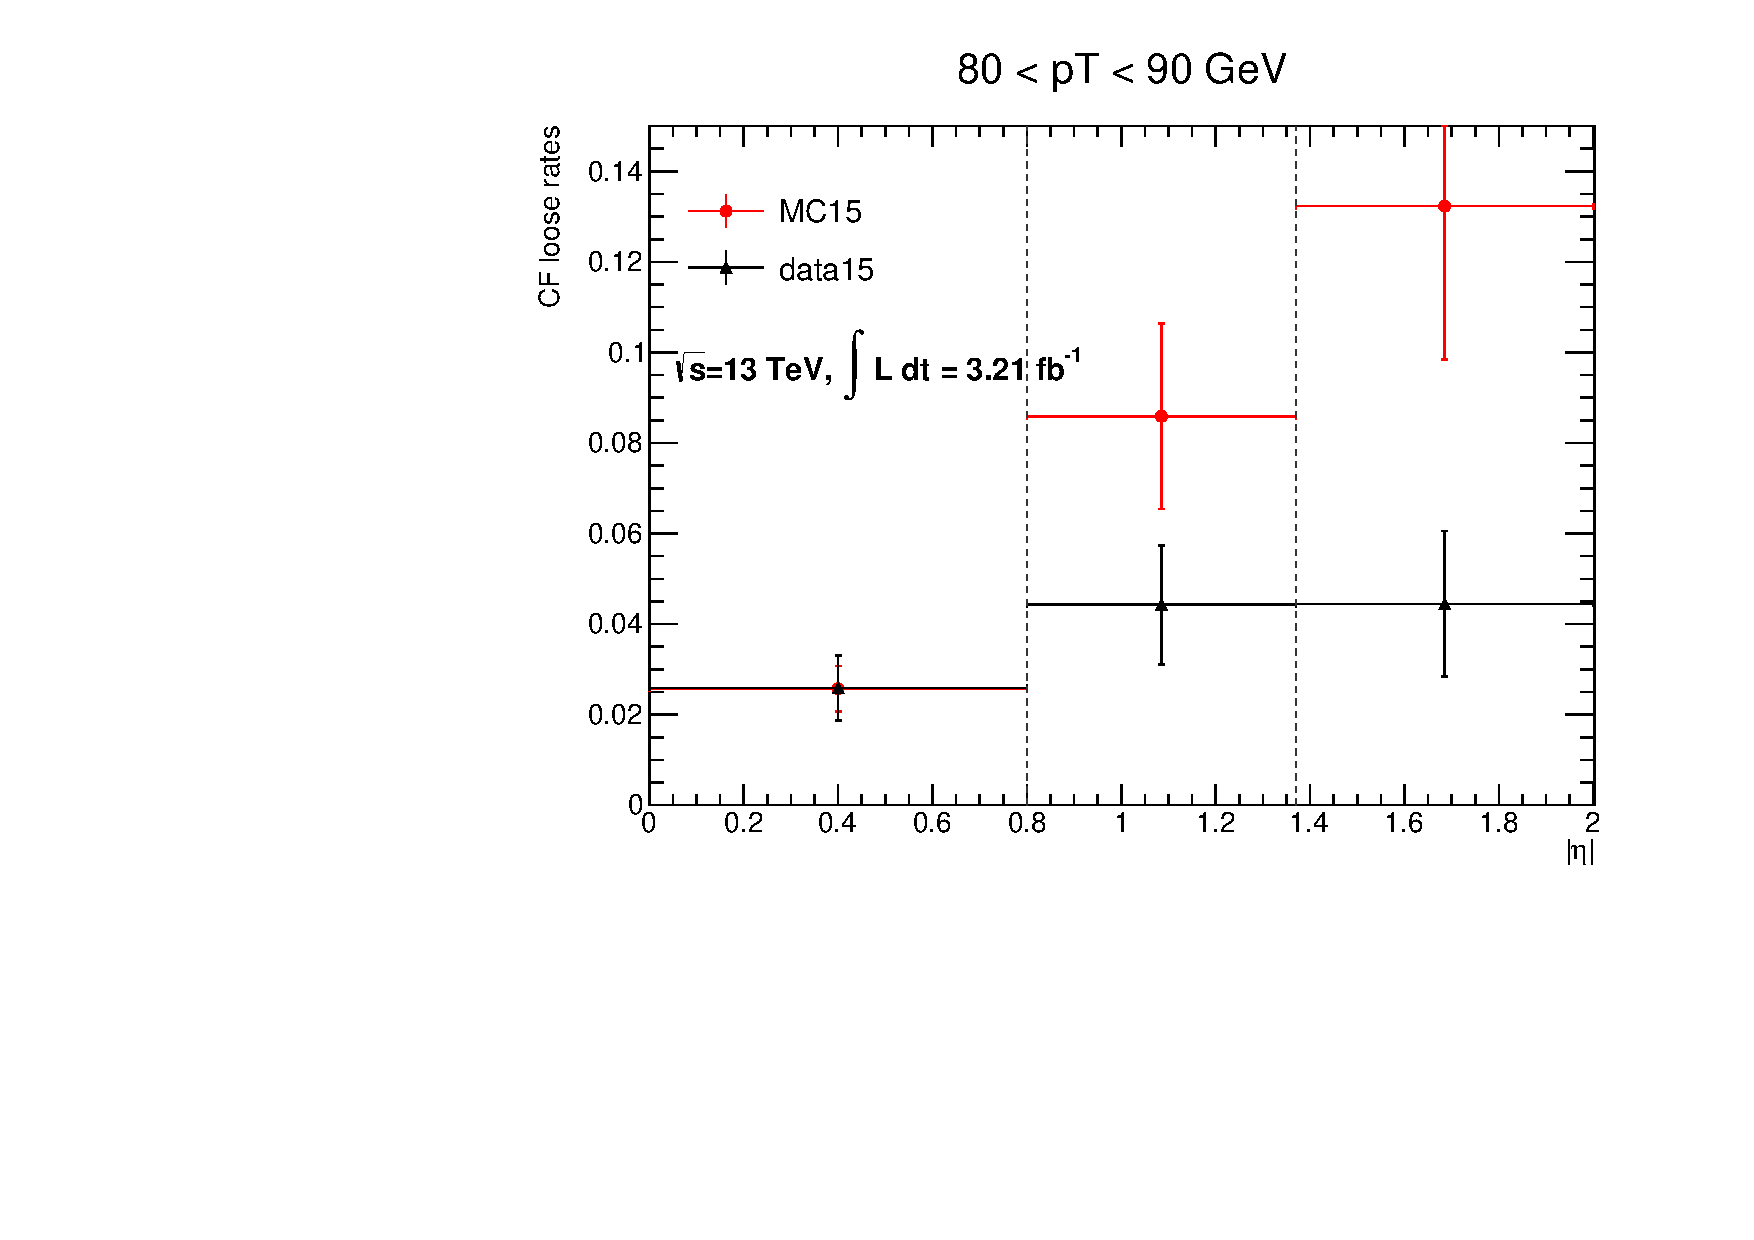
\includegraphics[width=0.4\textwidth]{FIGURES/BKG/chargeFlip/CFratesLOOSE___dataVSmc___PTbin7.pdf}
\vfill
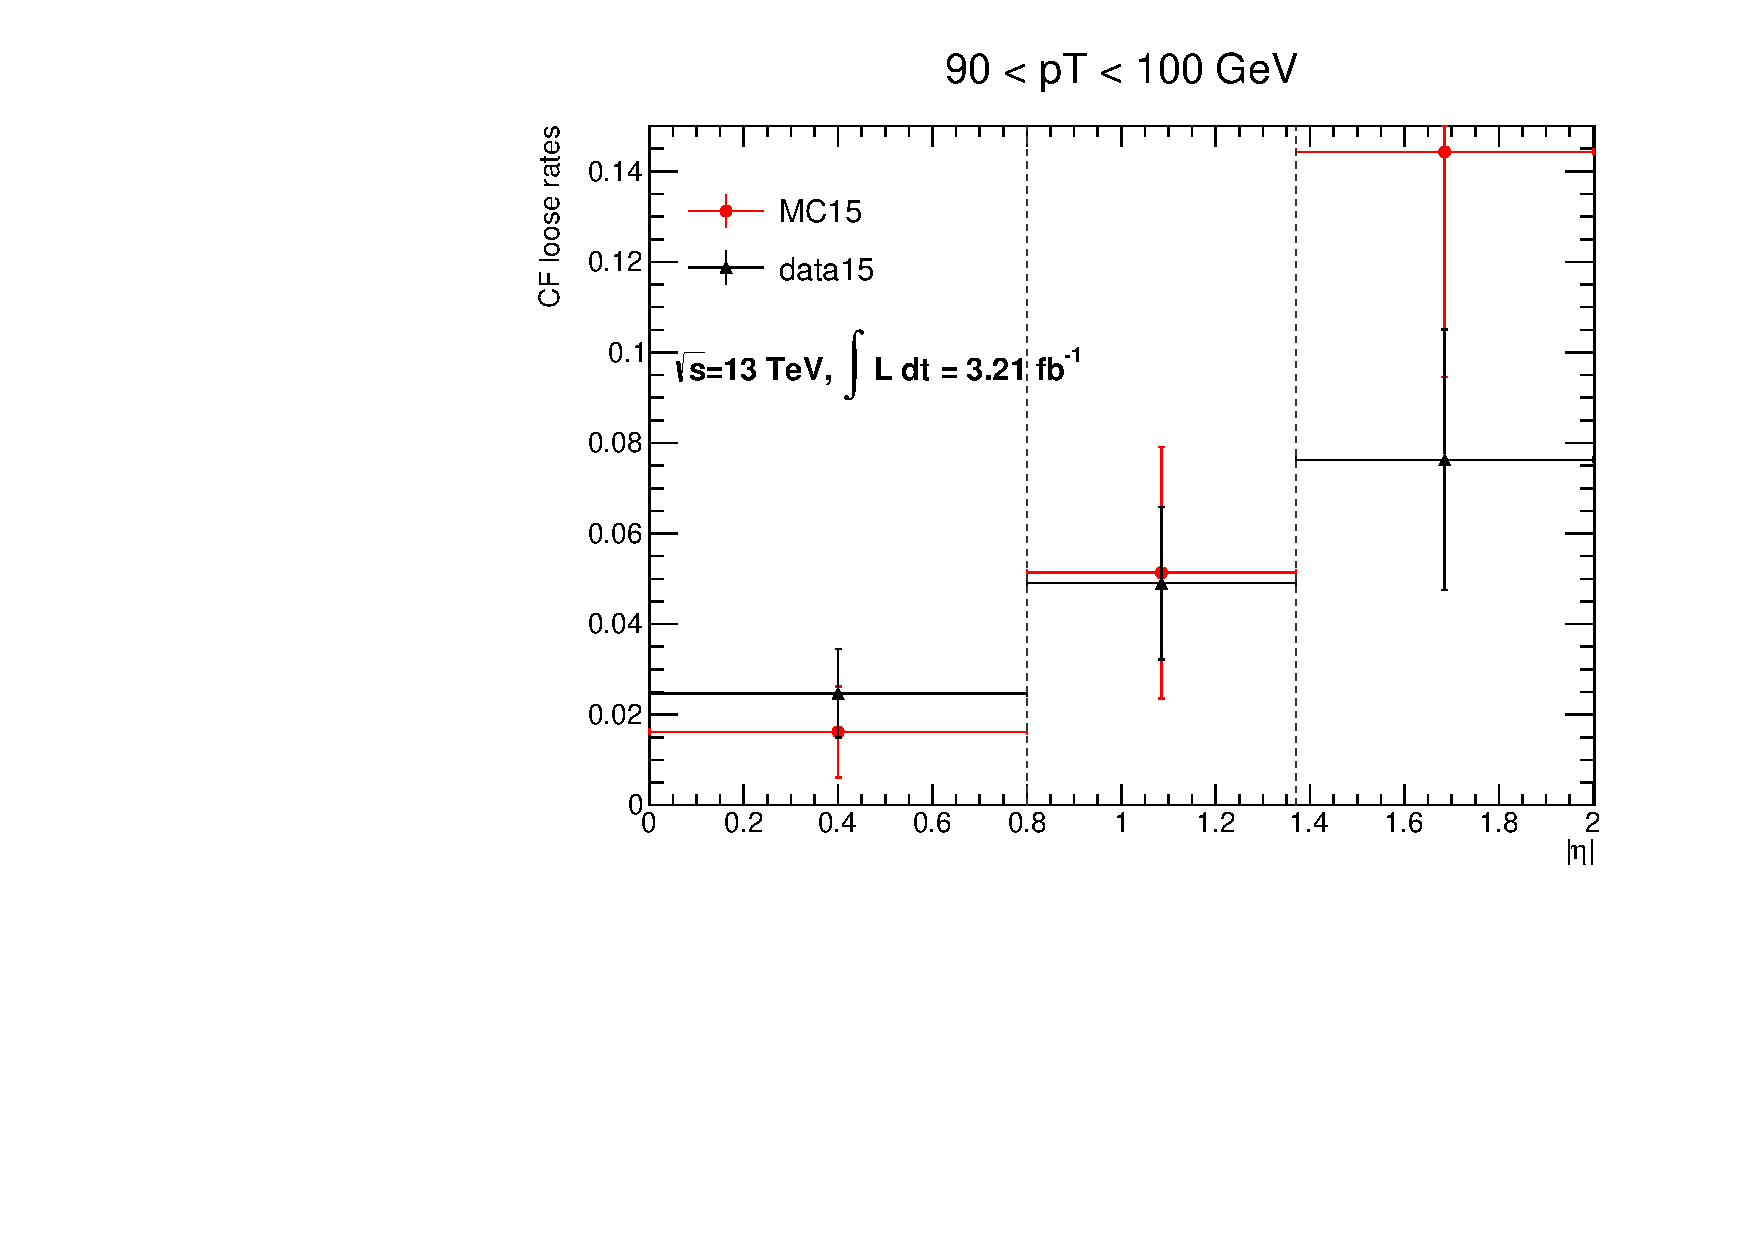
\includegraphics[width=0.4\textwidth]{FIGURES/BKG/chargeFlip/CFratesLOOSE___dataVSmc___PTbin8.pdf}
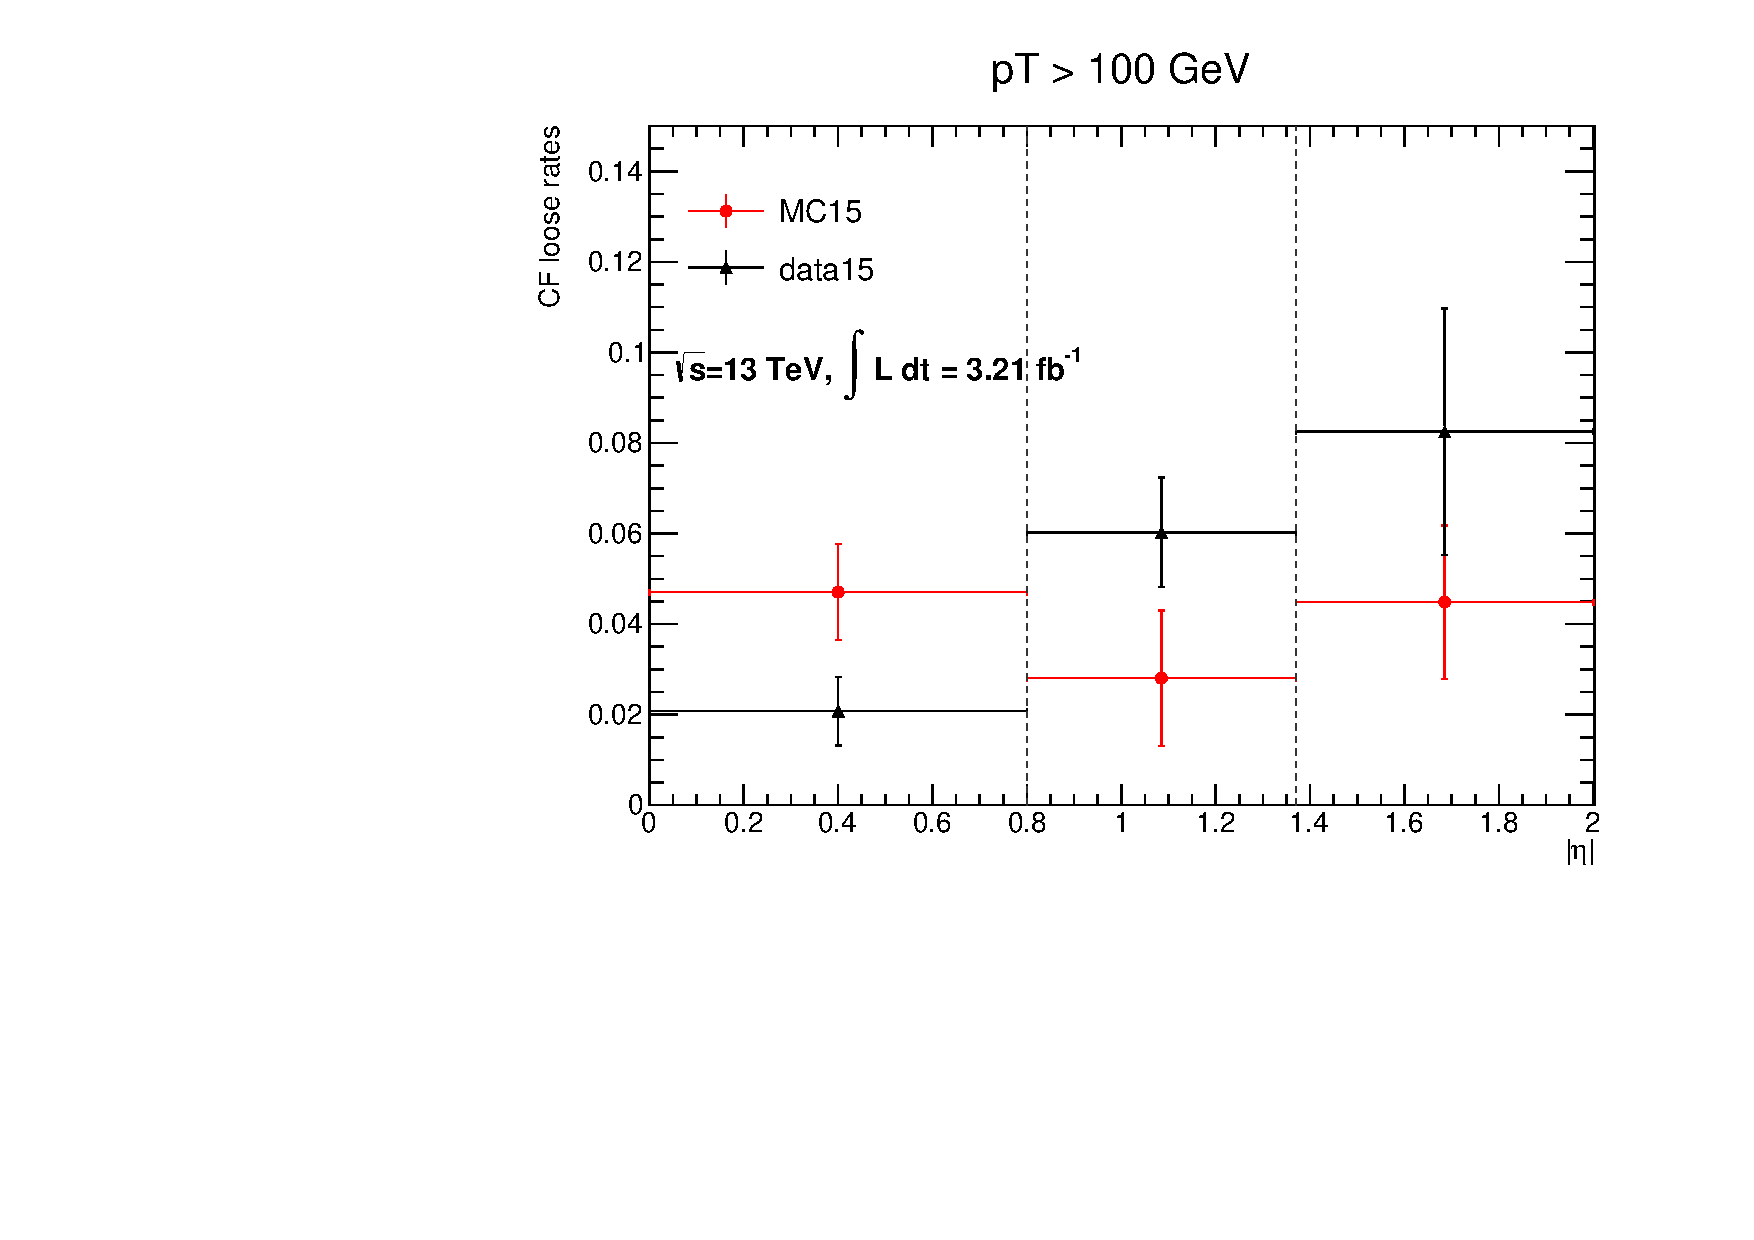
\includegraphics[width=0.4\textwidth]{FIGURES/BKG/chargeFlip/CFratesLOOSE___dataVSmc___PTbin9.pdf}
\caption{\label{fig:CFratesLoose_2} Charge flip rates extracted from data (black dots) and from MC $Z\to e^+e^-$ (red dots) for electrons failing the signal requirements, as a function of $\eta$ and in various $\pt$ bins. Statistical and systematic uncertainties are shown.}
\end{figure}
%------------------------------------------------
\FloatBarrier


\subsubsection{Systematics}
\label{subsec:CFsysSection}

The uncertainties on the charge mis-identification rates coming from the background subtraction procedure are computed and assigned as systematics. As mentioned in the previous section, the standard measurement is computed using a central-band width of $75<m_{ee}<100$~GeV and side-band regions of 25~GeV for the background subtraction. To evaluate the systematics, the charge flip rates were extracted for five different configurations: 
\begin{enumerate}
\item $75<m_{ee}<100$~GeV, no background subtraction; 
\item $75<m_{ee}<100$~GeV, side-band of 20~GeV;
\item $75<m_{ee}<100$~GeV, side-band of 25~GeV (standard measurement);
\item $75<m_{ee}<100$~GeV, side-band of 30~GeV; 
\item $80<m_{ee}<110$ GeV GeV, side-band of 25 GeV
\end{enumerate}
We then extract four different variations by comparing those five configurations. The effect of applying the background subtraction itself (called background ON and OFF) is computed by comparing configurations 1 vs. 3. The Z mass window width effects are computed by comparing configurations 3 vs. 5, while the side-band width effects are calculated by comparing configuration 3 vs. 2 and 3 vs. 4. Then the largest deviation in each bins is taken as the systematic uncertainty on the charge flip rates. 

Those variations are shown on Figure~\ref{fig:CFsys} for a $\pt$ range of 20-30 GeV for both type of events where electrons satisfied the signal requirements on left and where electrons don't satisfied the signal requirements (auxiliary measurement) on right. The black dots represent the standard measurement and coloured dots represent the different configurations used to compute the systematics. Figure~\ref{fig:CFsysTot} shows the total systematic uncertainties in each $[\pt,\eta]$ bin after combining the different contributions associated to the background subtraction method. The upper plot stand for the electron passing the signal requirements while lower plot is for electrons failing the signal requirements.

\begin{figure}[htb!]
\centering
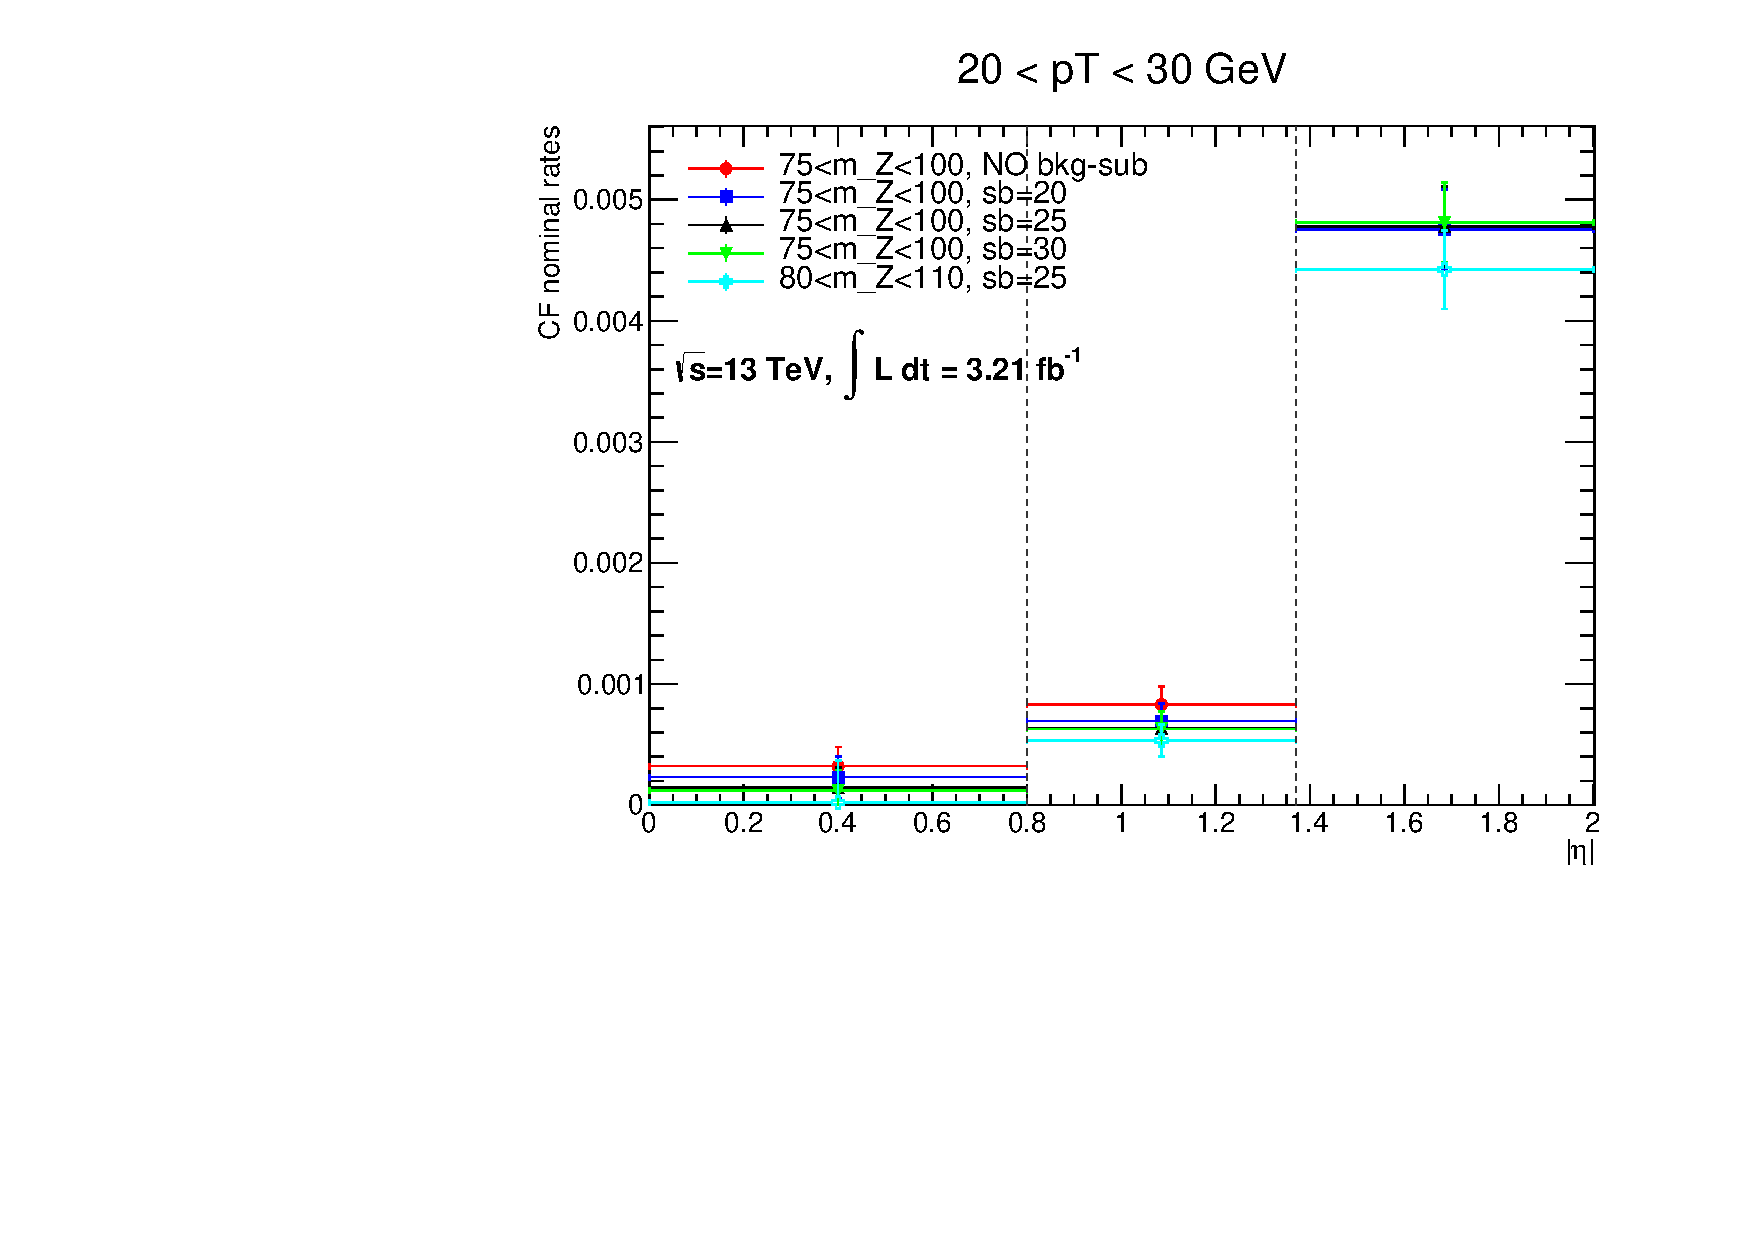
\includegraphics[width=0.48\textwidth]{FIGURES/BKG/chargeFlip/CFrates___SYStypes___PTbin1.pdf}
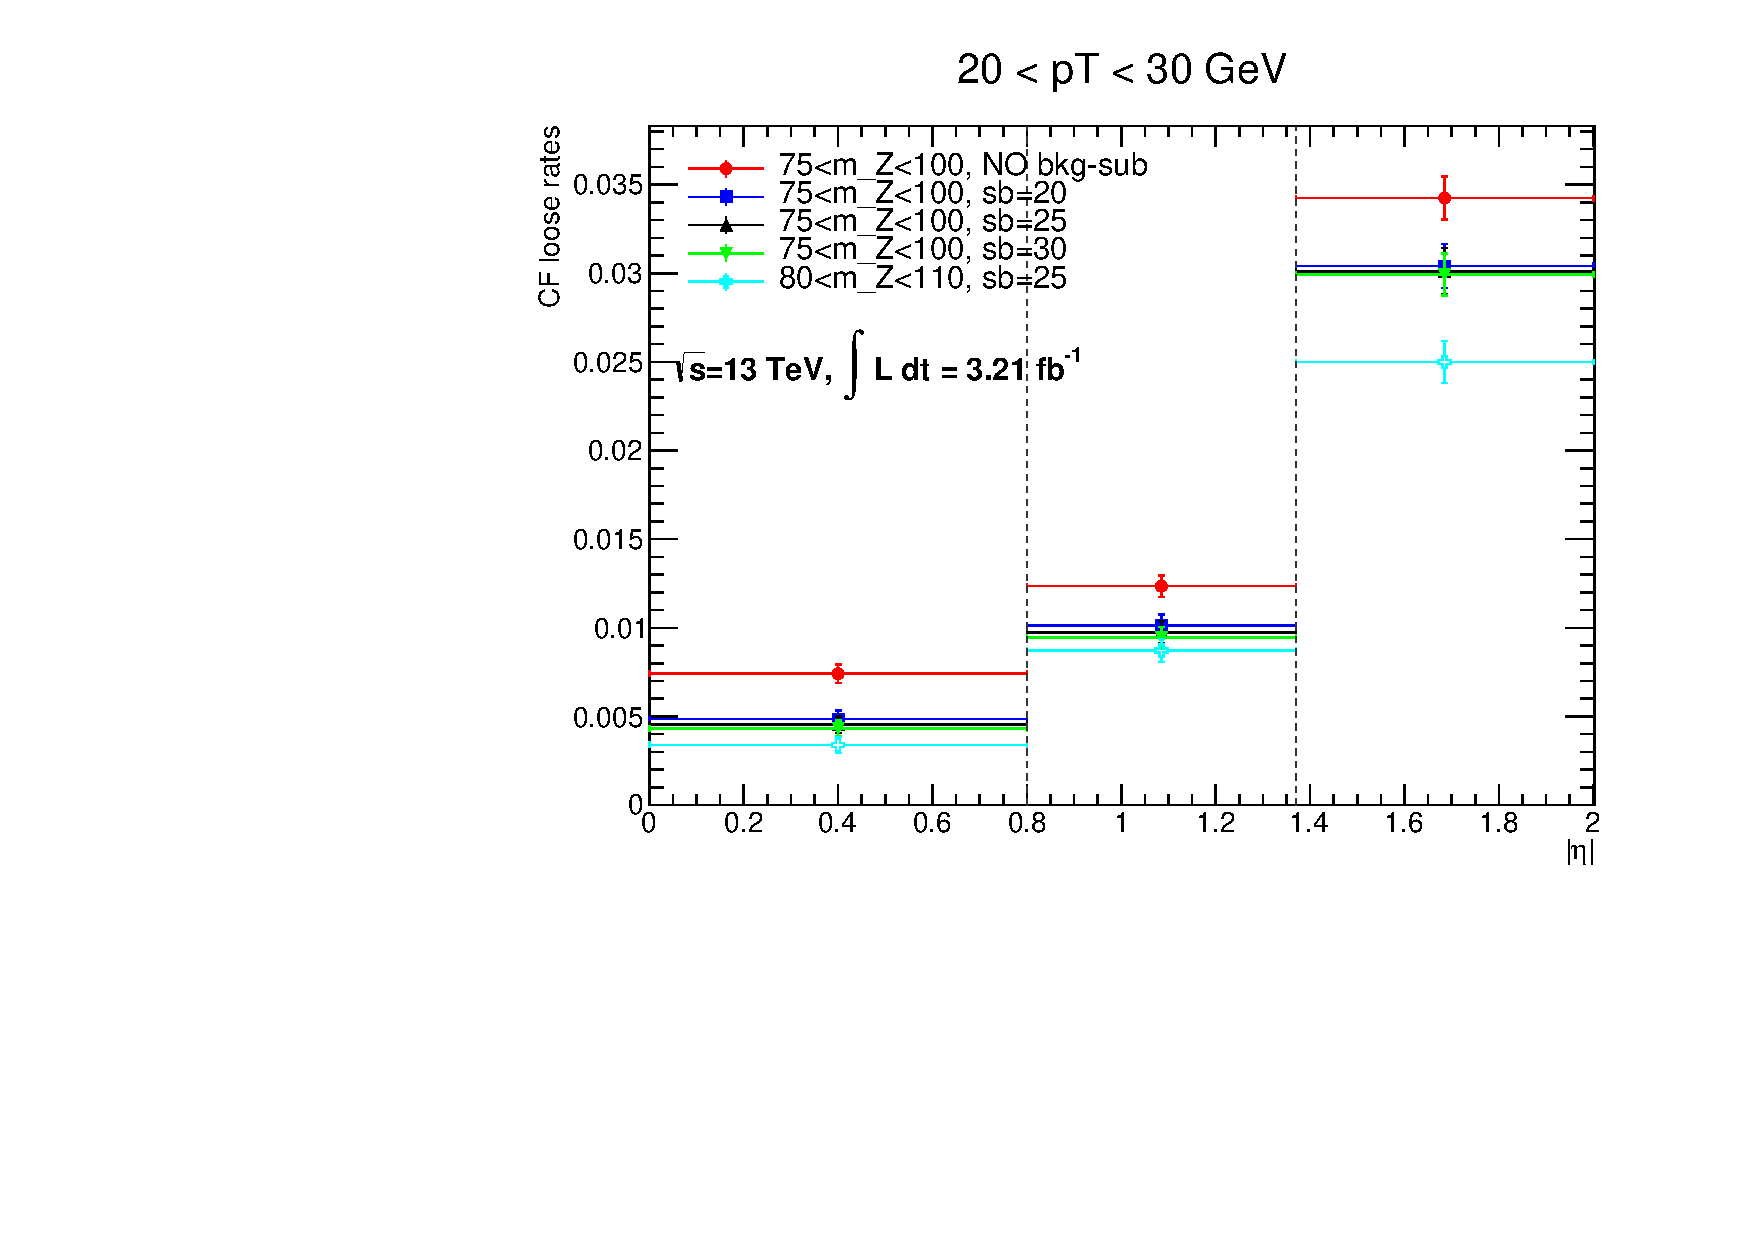
\includegraphics[width=0.48\textwidth]{FIGURES/BKG/chargeFlip/CFratesLOOSE___SYStypes___PTbin1.pdf}
\caption{\label{fig:CFsys} Charge flip rates in data for $20<\pt<30$ GeV bin using five different configurations of background subtraction for electrons satisfying the signal requirements on left handed plot and for electrons failing the signal requirements on the right handed plot. In each bin the largest deviation from the standard measurement (black dots) is taken to be the systematic uncertainty.}
\end{figure}

\begin{figure}[h!]
\centering
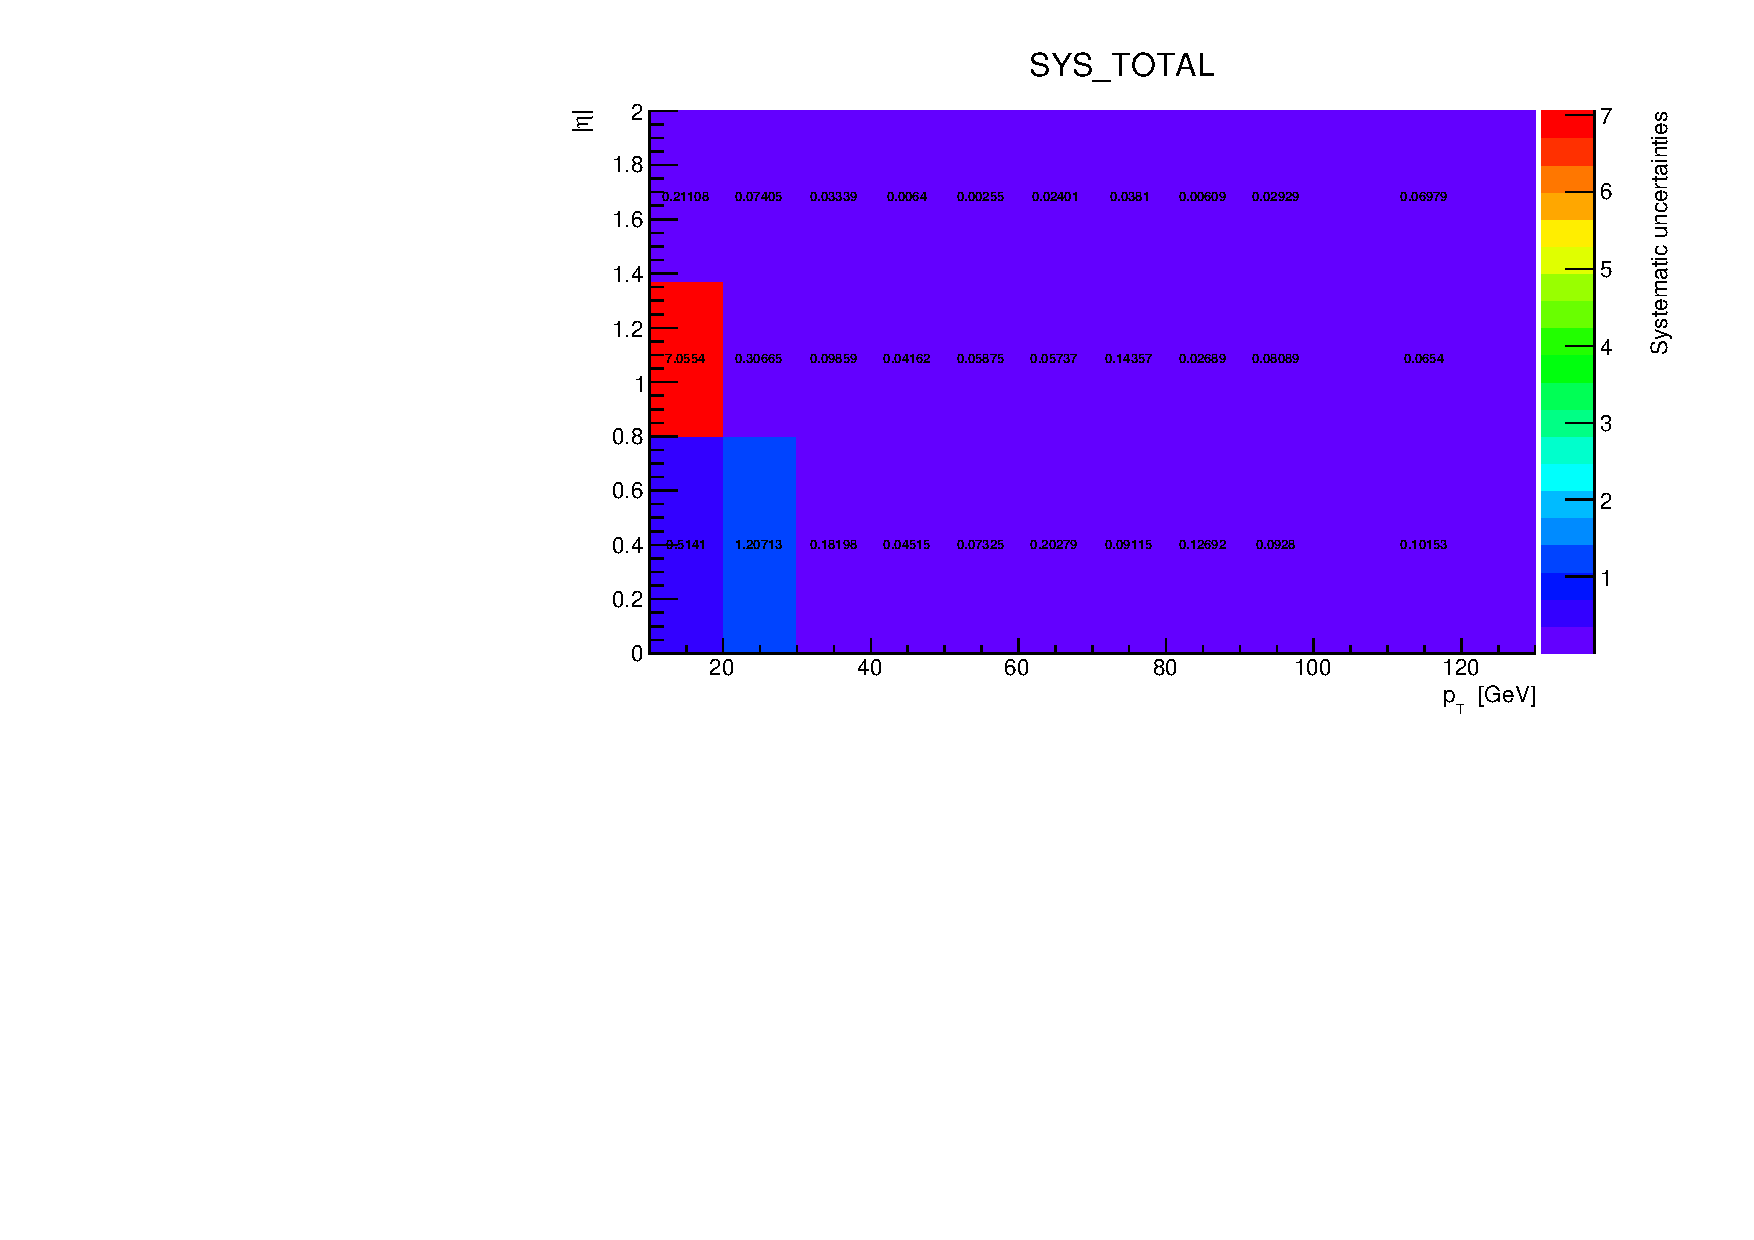
\includegraphics[width=0.65\textwidth]{FIGURES/BKG/chargeFlip/2D_histo_SYS_TOTAL.pdf}
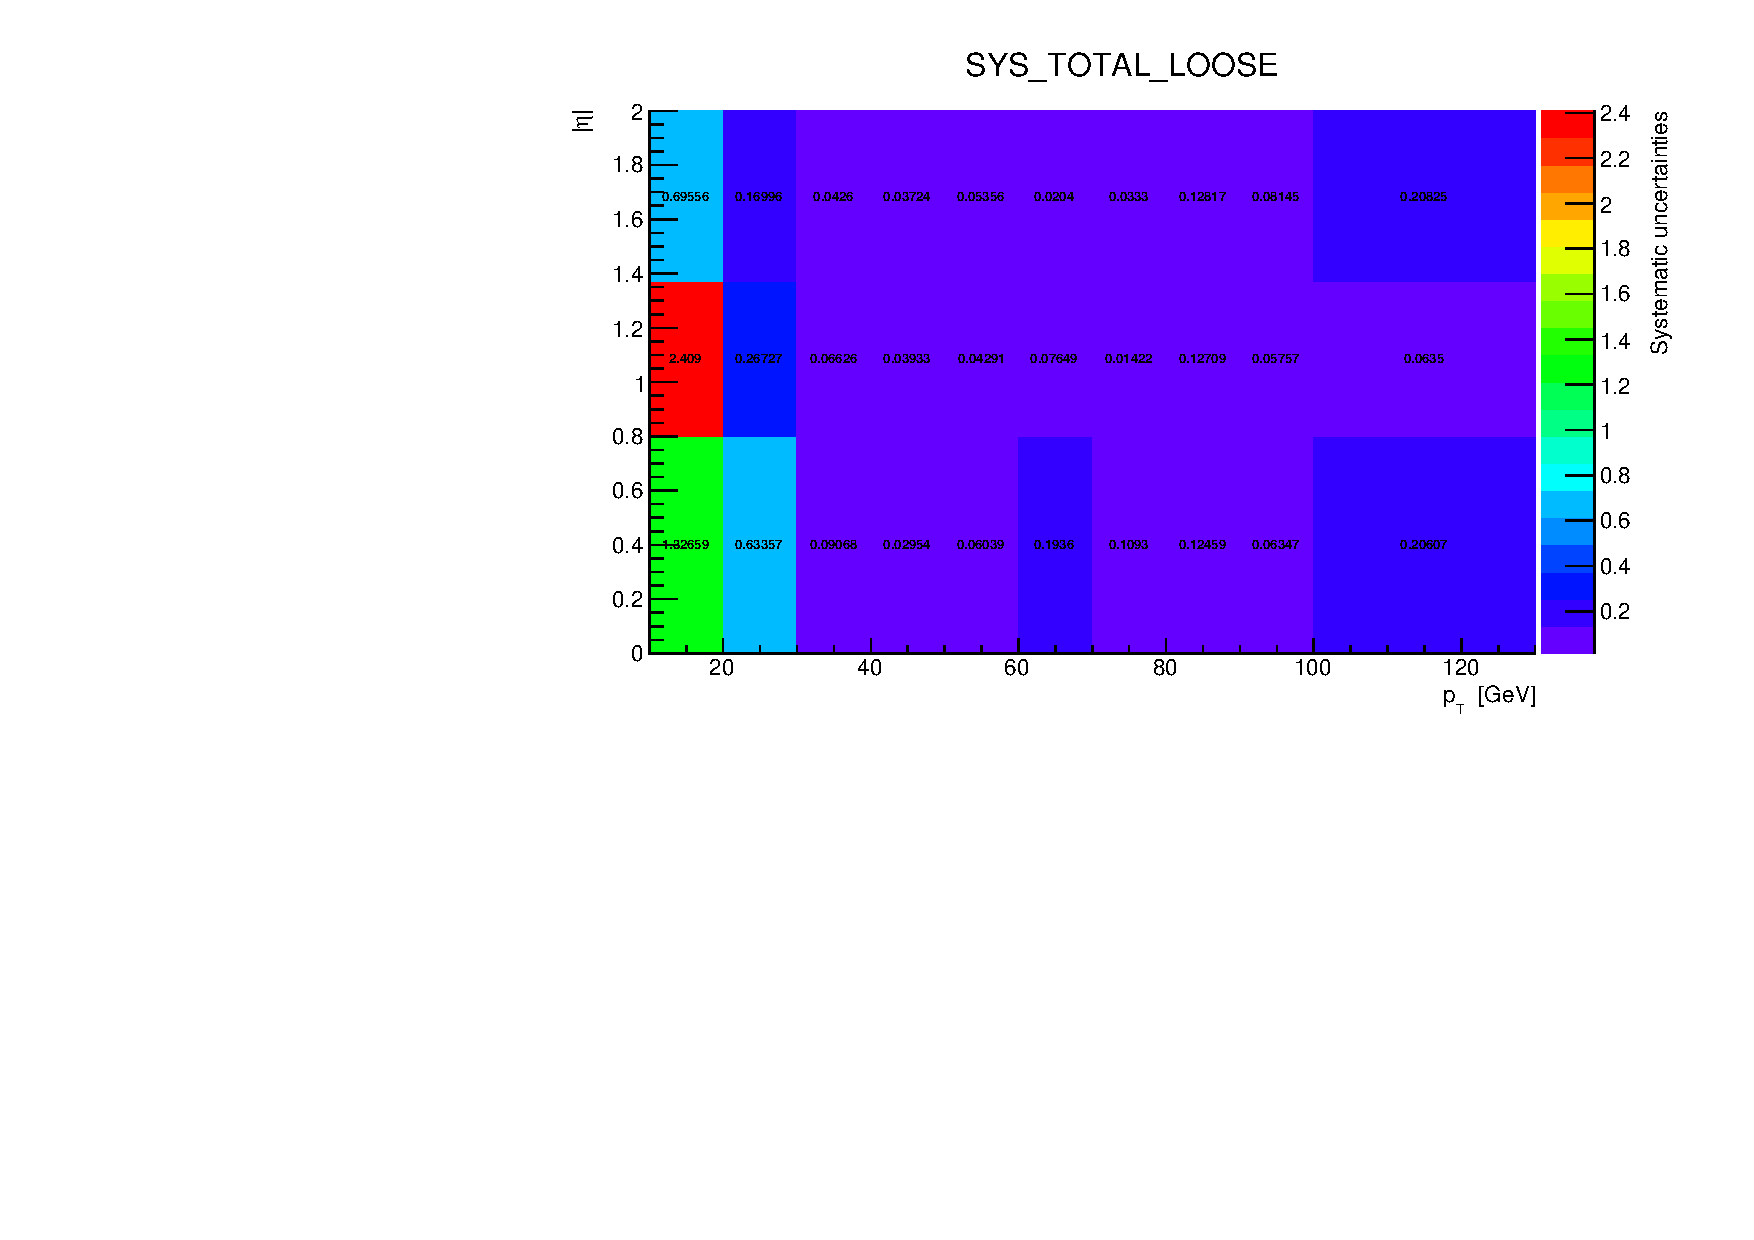
\includegraphics[width=0.65\textwidth]{FIGURES/BKG/chargeFlip/2D_histo_SYS_TOTAL_LOOSE.pdf}
\caption{\label{fig:CFsysTot} Total systematic uncertainties evaluated in each bins by taking the largest deviation coming from the comparison of different configurations in background subtraction method (in data) for electrons satisfying the signal requirements on the upper plot and for electrons failing the signal requirements on the lower plot.}
\end{figure}


%%%%%%%%%%%%%%%%%%%%%%%%%%%%%
\subsection{Backgrounds with fake leptons: general information}
\label{sec:bkg_fakes} 
The term ``fake lepton'' denotes here generically non-prompt leptons produced in heavy flavor meson decays, 
converted photons, light hadrons faking the electron shower, in-flight decays of kaons or pions to muons, etc.  
Common properties shared by these objects are a bad response to the electron/muon identification cuts, 
non-zero impact parameters, and the reconstructed leptons are often not well isolated. 
These properties can be used to discriminate the fake leptons against the prompt and isolated leptons we are interested in (and which we call ``real leptons''). 

We rely on two different and complementary methods to estimate the fake leptons yields in the signal regions, 
either purely data-driven or relying on the MC simulations, 
which are described respectively in Sections~\ref{sec:bkg_matrix_method} and~\ref{sec:bkg_mctemplate_method}; 
we also cross-check the fake background estimate for the special case of the SR3b signal region with a third method described in section~\ref{sec:bkg_abcd_method}. 
First two methods have already been employed successfully in the Run-1 analysis~\cite{noteSS3L}. 
The rest of this section provides some details about the dominant sources of fake leptons close to the signal regions according to the simulations predictions. 


%%%%%%%%%%%%%%%%%%%%%%%%%%%%%
\subsubsection{Fake lepton sources close to the signal regions} 
\label{sec:truthComposition_SR}

We studied in the MC simulations the sources of fake leptons close to the signal regions, which we briefly summarize here. 
This information is important notably for the setup of the related background estimate (the matrix method) and the assignment of systematic uncertainties. 
It is also genuinely interesting as it may help further rejecting fake leptons by focusing on the relevant source and devising appropriate discriminants. 

Ideally we would study directly the composition of the signal regions; 
however, the limited MC statistics does not really allow to do so with a high level of confidence on the results. 
Therefore, to have more reliable conclusions, we performed these studies in a set of regions with relaxed selection criteria compared to the signal regions (i.e. no \meff\ cut, looser cuts on ($b$-) jet multiplicity and \met, etc.). 
Such criteria are detailed in Table~\ref{tab:TruthComposition_SR}. 
However, the conclusions obtained in this section can be extrapolated to the signal regions, 
notably since the source of fake leptons due to $t\bar t$ processes dominates over other sources both in the relaxed and in the ``nominal'' signal regions. 

The sources of fake leptons are identified through the classification performed by the \texttt{MCTruthClassifier} tool, 
following the approach defined in section~\ref{sec:truth_matching}. 
In this present section, only \ttbar\ and $V$+jets Monte Carlo samples (as presented in Section~\ref{sec:BGSamples}) are analysed, 
since we expected the other potential sources (QCD processes such as $pp\to b\bar b$, diboson\ldots) to be very minor in the signal regions. 
To increase the available statistics, we did not apply the requirements on the charges of the leptons here. 

\begin{table}[h!]
\caption{The relaxed signal regions used to study the origin of fake leptons in simulation.}
\hspace{0.5cm}
\label{tab:TruthComposition_SR}
\centering
%\resizebox{0.8\textwidth}{!}{
\begin{tabular}{|c|c|c|c|}
\hline
\hline
Signal region  &      $N_{lept}$             & $N_{b-jets}^{20}$               & Other variables \\
\hline
\hline
SR0b &  $\ge$2  &    $==$0        &     $N_{jets}^{25} \ge$ 3, \met\ ~$>$~70 \GeV \\
\hline
SR1b     &  $\ge$2  &    $\ge$1        &     $N_{jets}^{25} \ge$ 3, \met\ ~$>$~70 \GeV \\
\hline
SR2b     &   $\ge$2  &   $\ge$2        &   -    \\
\hline
\end{tabular}%}
\end{table}
 

\par{\bf Fake electron sources\\}
The fake electrons are classified in a few general categories depending on the origin of the electron 
(conversion from prompt photons, light hadron fakes including $\pi^0\to\gamma\gamma$, non-prompt taus, bottom and charm meson semileptonic decays). 
The relative abundances of these sources are shown in Fig~\ref{Fig:truthComposition_EL_by_source_vs_pt} for different $p_T$ cuts on the electrons, 
in the relaxed signal regions defined in Table~\ref{tab:TruthComposition_SR}. 
They are presented for both baseline and signal electrons definitions~--~the former being useful to understand the events input to the matrix method in the signal regions. 
For completeness, the number of events in each category and the associated statistical uncertainties 
are shown in Appendix~\ref{App:FakeLep} (Fig~\ref{Fig:truthComposition_EL_by_source_vs_pt_MORE}). 
The dependency on other kinematic variables like \met, \meff, etc. is shown in the same appendix. 

Generally a strong dependency is observed on the fake electron \pt. 
At the baseline level, in the relaxed SR0b and SR1b regions 
the dominant sources of fake electrons arise from both light hadron fakes and bottom hadrons decays; 
however, at the signal level the dominant source is the bottom hadrons decays, beside at high \pt\ ($>$30~\GeV) where the light flavor sources are higher than 30\%. In a selection with $\ge 2$ $b$-jets, most of the fakes arise from light hadrons decays.
%, apart in the low \pt region (as low as 10~\GeV) at signal level where bottom decays contribute equally.

Fig~\ref{Fig:truthComposition_EL_pT_spectrum} presents the $p_T$ spectrum of the fake electrons in the relaxed signal regions, 
distinguishing the $t\bar t$ and $V+$ jets processes. 
In all signal regions the background will be dominated by fake electrons from \ttbar processes. 
The first \pt bin ($p_T<20$ GeV) is depleted since due to the $p_T$ requirements in the lepton selection, 
only events with three leptons may fill this bin, which are less frequent in \ttbar. 

\begin{figure}[p]
\centering
\subfigure[Baseline electrons, ``relaxed'' SR0b] 
{\includegraphics[width=0.49\textwidth]{Truth_Composition/Baseline/Vj_1EL_pT_Var_DEF4.pdf}}
\subfigure[Signal electrons, ``relaxed'' SR0b]{
\includegraphics[width=0.49\textwidth]{Truth_Composition/Signal/Vj_1EL_pT_Var_DEF4.pdf}
}
\subfigure[Baseline electrons, ``relaxed'' SR1b]
{\includegraphics[width=0.49\textwidth]{Truth_Composition/Baseline/Vj_1EL_pT_Var_DEF5.pdf}}
\subfigure[Signal electrons, ``relaxed'' SR1b]{
\includegraphics[width=0.49\textwidth]{Truth_Composition/Signal/Vj_1EL_pT_Var_DEF5.pdf}
}
\subfigure[Baseline electrons, ``relaxed'' SR2b]
{\includegraphics[width=0.49\textwidth]{Truth_Composition/Baseline/Vj_1EL_pT_Var_DEF6.pdf}}
\subfigure[Signal electrons, ``relaxed'' SR2b]{
\includegraphics[width=0.49\textwidth]{Truth_Composition/Signal/Vj_1EL_pT_Var_DEF6.pdf}
}
\caption
{Sources of fake electron as a function of the electron $p_T$, as predicted by MC simulations (combined $t\bar t$ and $V+$ jets) 
in the relaxed signal regions defined in Table~\ref{tab:TruthComposition_SR}. The results are shown for baseline (left) or signal electrons (right).} 
\label{Fig:truthComposition_EL_by_source_vs_pt}
\end{figure}
%%
\begin{figure}[p]
\centering
\subfigure[Baseline electrons, ``relaxed'' SR0b]
{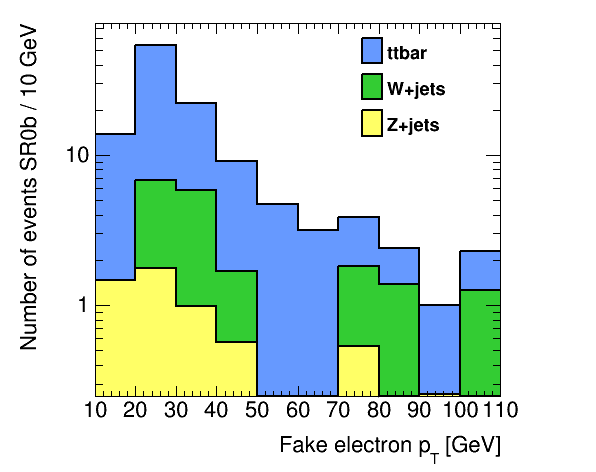
\includegraphics[width=0.49\textwidth]{Truth_Composition/BaseEL_SR0bPt}}
\subfigure[Signal electrons, ``relaxed'' SR0b]{
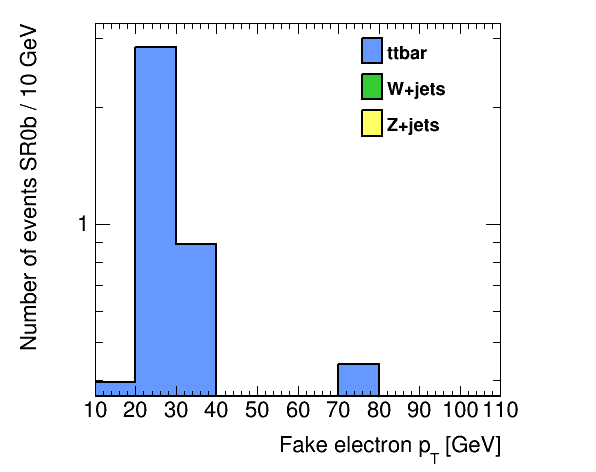
\includegraphics[width=0.49\textwidth]{Truth_Composition/SigEL_SR0bPt}
}
\subfigure[Baseline electrons, ``relaxed'' SR1b]
{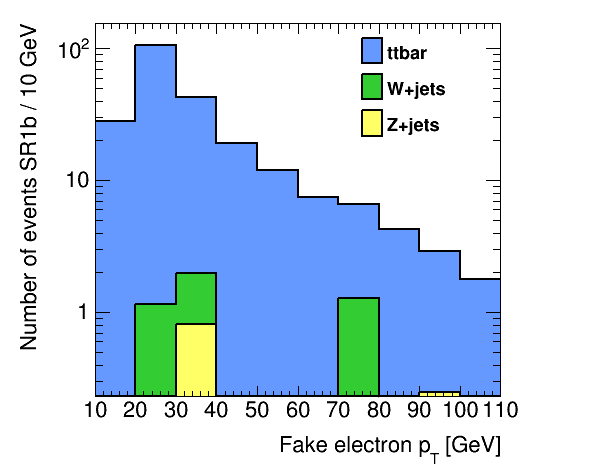
\includegraphics[width=0.49\textwidth]{Truth_Composition/BaseEL_SR1bPt}}
\subfigure[Signal electrons, ``relaxed'' SR1b]{
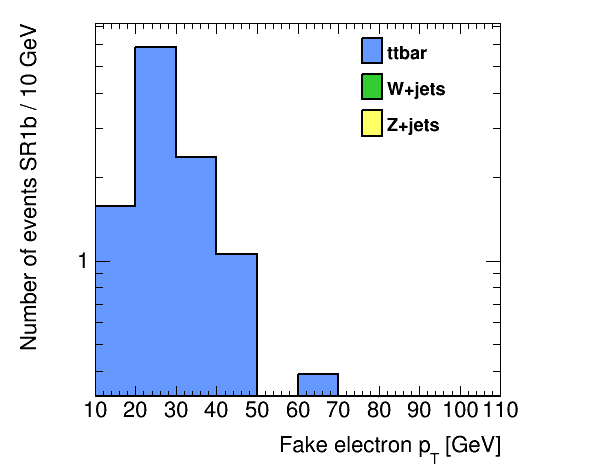
\includegraphics[width=0.49\textwidth]{Truth_Composition/SigEL_SR1bPt}
}
\subfigure[Baseline electrons, ``relaxed'' SR2b]
{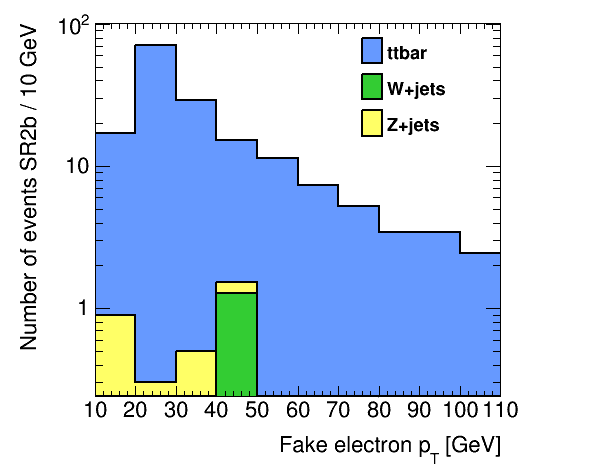
\includegraphics[width=0.49\textwidth]{Truth_Composition/BaseEL_SR2bPt}}
\subfigure[Signal electrons, ``relaxed'' SR2b]{ 
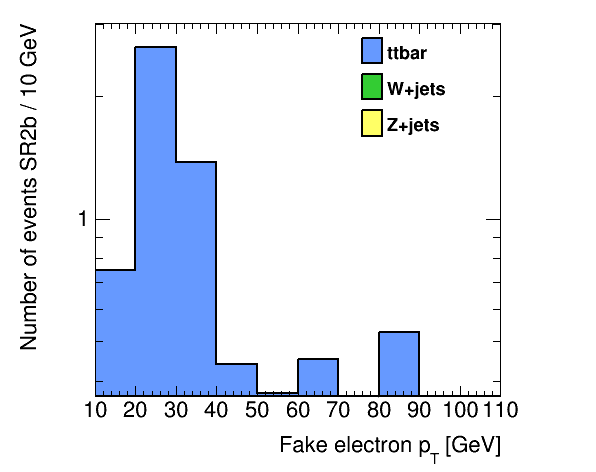
\includegraphics[width=0.49\textwidth]{Truth_Composition/SigEL_SR2bPt}
}
\caption
{Transverse momentum distribution of the fake electrons as predicted by MC simulations in the relaxed signal regions defined in Table~\ref{tab:TruthComposition_SR}. Electrons originating from $t\bar t$ or $V+$ jets events are distinguished. }
\label{Fig:truthComposition_EL_pT_spectrum}
\end{figure}


\par{\bf Fake muon sources\\}
We classified fake muons into four categories, according to the decision of the \texttt{MCTruthClassifier} tool, and depending on the heavy flavor content of the hadron at the origin of the muon (light, tau, bottom and charm). We show the relative abundances of these sources in Fig~\ref{Fig:truthComposition_MU_by_source_vs_pt} for different $p_T$ cuts on the muons, in the relaxed signal regions defined in Table~\ref{tab:TruthComposition_SR}. They are presented for both baseline and signal muons definitions. The number of events in each category and the associated statistical uncertainties are shown in Appendix~\ref{App:FakeLep} (Fig~\ref{Fig:truthComposition_MU_by_source_vs_pt_MORE}). The dependency of other kinematic variables like \met, \meff, etc. is shown in the same appendix.

One can see that the dominant source are always non-prompt muons arising from charmed or bottom hadron decays, in all \pt regions. In general, the non-prompt muons come mainly from $b$-sources (the fraction of such events is around 70$\%$ or more), 
except in the SR2b selection: this is interpreted as the fact that in $t\bar t$ events, tagging the 2 $b$-jets (as is required in this region) strongly reduces the rate of non-prompt muons originating from these, as the small impact parameter required for that muon to satisfy signal cuts contradicts the $b$-jet tagging which relies on the presence of displaced tracks and a secondary vertex. Fig~\ref{Fig:truthComposition_MU_pT_spectrum} presents the $p_T$ spectrum of these fake muons in the relaxed signal regions, distinguishing the $t\bar t$ and $V+$ jets processes. For all selections, the background will be dominated by low $p_T$ fake muons originating from $t\bar t$. 

\begin{figure}[p]
\centering
\subfigure[Baseline muons, ``relaxed'' SR0b]
{\includegraphics[width=0.49\textwidth]{Truth_Composition/Baseline/Vj_1MU_pT_Var_DEF4.pdf}}
\subfigure[Signal muons, ``relaxed'' SR0b]{
\includegraphics[width=0.49\textwidth]{Truth_Composition/Signal/Vj_1MU_pT_Var_DEF4.pdf}
}
\subfigure[Baseline muons, ``relaxed'' SR1b]
{\includegraphics[width=0.49\textwidth]{Truth_Composition/Baseline/Vj_1MU_pT_Var_DEF5.pdf}}
\subfigure[Signal muons, ``relaxed'' SR1b]{
\includegraphics[width=0.49\textwidth]{Truth_Composition/Signal/Vj_1MU_pT_Var_DEF5.pdf}
}
\subfigure[Baseline muons, ``relaxed'' SR2b]
{\includegraphics[width=0.49\textwidth]{Truth_Composition/Baseline/Vj_1MU_pT_Var_DEF6.pdf}}
\subfigure[Signal muons, ``relaxed'' SR2b]{
\includegraphics[width=0.49\textwidth]{Truth_Composition/Signal/Vj_1MU_pT_Var_DEF6.pdf}
}
\caption
{Sources of fake muons as a function of the muon $p_T$, as predicted by MC simulations (combined $t\bar t$ and $V+$ jets) 
in the relaxed signal regions defined in Table~\ref{tab:TruthComposition_SR}. The results are shown for baseline (left) or signal muons (right).}
\label{Fig:truthComposition_MU_by_source_vs_pt}
\end{figure} 
%%
\begin{figure}[p]
\centering
\subfigure[Baseline muons, ``relaxed'' SR0b]
{\includegraphics[width=0.49\textwidth]{Truth_Composition/BaseMU_SR0bPt}}
\subfigure[Signal muons, ``relaxed'' SR0b]{
\includegraphics[width=0.49\textwidth]{Truth_Composition/SigMU_SR0bPt} 
}
\subfigure[Baseline muons, ``relaxed'' SR1b]
{\includegraphics[width=0.49\textwidth]{Truth_Composition/BaseMU_SR1bPt}}
\subfigure[Signal muons, ``relaxed'' SR1b]{
\includegraphics[width=0.49\textwidth]{Truth_Composition/SigMU_SR1bPt}
}
\subfigure[Baseline muons, ``relaxed'' SR2b]
{\includegraphics[width=0.49\textwidth]{Truth_Composition/BaseMU_SR2bPt}}
\subfigure[Signal muons, ``relaxed'' SR2b]{
\includegraphics[width=0.49\textwidth]{Truth_Composition/SigMU_SR2bPt}
}
\caption
{Transverse momentum distribution of the fake muons as predicted by MC simulations in the relaxed signal regions defined in Table~\ref{tab:TruthComposition_SR}. Muons originating from $t\bar t$ or $V+$ jets events are distinguished. }
\label{Fig:truthComposition_MU_pT_spectrum}
\end{figure} 

%%%%



%%%%%%%%%%%%%%%%%%%%%%%%%%%%%
\subsection{Backgrounds with fake leptons: the matrix method}
\label{sec:bkg_matrix_method}
The matrix method is a purely data-driven approach used to estimate the amount of fake leptons in the regions of interest (i.e. validation regions, signal regions, etc). It relies on the different response of the prompt and fake leptons to identification, isolation and impact parameters requirements: the fake leptons have low probabilities to satisfy these requirements, unlike the prompt leptons. 
No attempt is made to consider the different categories of fake leptons separately for the extraction of fake rates, but systematic uncertainties are assigned to cover possible differences. 

\par{\bf Methodology\\}
A combination of tight requirements on discriminant variables such as the electron identification, the lepton isolation and impact parameters is defined (see Tabe~\ref{tab:lepdef}). The reconstructed leptons are then classified in two categories ("tight" and "loose"), depending on their success satisfying the tight requirements or not. If $\epsilon$ and $\zeta$ are respectively the probabilities for a prompt/fake lepton to satisfy the requirements, linear relationships can be established between the mean values of the rates of prompt/fakes and tight/loose leptons, which for the 1-lepton case are: 
\begin{align}
\label{eqn:matrixmethod}
<N_\text{tight}> &= \epsilon <N_\text{prompt}> + \zeta <N_\text{fake}> \\\notag
<N_\text{loose}> &=  (1-\epsilon) <N_\text{prompt}> + (1-\zeta) <N_\text{fake}>
\end{align}

This system of equations can be used to evaluate the number of prompt and fake leptons given the observed number of tight and loose leptons. 
In this analysis we are using a generalization of this method, able to handle events with arbitrary number of leptons -- the well know dynamic matrix method. 
It was already used in the Run-1 analysis and is described in detail in~\cite{noteSS3L,TomThesis}. 

The method relies of the prior knowledge of the probabilities $\epsilon$ and $\zeta$, 
which need to be measured in dedicated samples enriched in prompt and fake leptons, as presented in Sections~\ref{sec:RealRate_DD} and~\ref{sec:FakeRate_DD}.
The uncertainties on the probabilities for fake leptons constitute the main source of uncertainties in the asymptotic regime. 
In the low statistics regime, one has to cope with the fact that the loose and tight leptons categories are not enough populated 
to provide reliable estimates: for example predictions of negative yields are a possible outcome. In general these estimates are accompanied by large statistical uncertainties. 

Finally, one should note that the charge flip electron background interferes with the matrix method 
as the charged flipped electrons are notably more prone to fail impact parameter or tight identification requirements, 
and the related efficiencies are distinct from both those of prompt and fake electrons. 
They correspond so to speak to a third category of objects, while the matrix method is based on the assumption that only two categories are present. One way to solve the issue is to rely on the linearity of the matrix method estimate with respect to its input number of events~: therefore one can simply subtract the estimated charge flip background in the tight and loose leptons categories, from the observed data. 
This requires a dedicated measurement of the charge flip rate for electrons failing the tight requirement (Section~\ref{sec:bkg_chflips}). 



%%%%%%%%%%%%%%%%%%%%%%%%%%
\subsubsection{Measurement of the $\epsilon$ probabilities (prompt leptons)}
\label{sec:RealRate_DD}
The real efficiency is measured in a high purity data sample with the standard $Z$ tag-and-probe method. The \texttt{HLT\_e24\_lhmedium\_iloose\_L1EM20VH} and \texttt{HLT\_mu20\_iloose\_L1MU15} single lepton triggers triggers are used to select the events. A tag lepton, used to identify the $Z\to \ell\ell$ process, should fulfil the signal leptons requirements (Table~\ref{tab:lepdef}), have a \pt larger than 25~GeV and be matched with the relevant single lepton trigger. An additional probe lepton, used for the efficiency measurement, should satisfy the baseline selection (Table~\ref{tab:lepdef}). For each tag-and-probe lepton pair both leptons are alternatively considered as the possible tag, as it allows to increase the statistics and to remove any bias in the choice of the tag. To enrich the selection in $Z\to \ell\ell$ events, the invariant mass of the tag-and-probe pairs is required to be in the $80 < m_{\ell\ell} < 100$~GeV interval. The efficiency is measured as a function of \pt and $\eta$\footnote{The electron efficiency $\eta$ binning is driven by the calorimeter geometry removing the calorimeter crack region.}. For illustration, Figure~\ref{Fig:InvMass_realEff} shows the invariant mass of the tag-and-probe pair distribution in data for events which pass or fail the signal cuts.        

\begin{figure}[h!]
\centering
\subfigure{
\includegraphics[width=0.45\textwidth]{BKG/realEff/OS_PASSFAIL_EL.pdf}
\includegraphics[width=0.45\textwidth]{BKG/realEff/OS_PASSFAIL_MU.pdf}
}
\caption{Invariant mass of the tag-and-probe electron (left) and muon (right) opposite-sign pair, for probes passing/failing the signal requirements. }
\label{Fig:InvMass_realEff}
\end{figure}

A sizable background contamination is observed for the $\pt < 20$ GeV electrons. This contamination is estimated using a background template method inspired by the one used by the $e/\gamma$ CP group to measure reconstruction and identification efficiencies measurements~\cite{ATLAS-CONF-2014-032}. Related systematic uncertainties are set by varying the $m_{ee}$ measurement window and the background template method. Besides, the \texttt{HLT\_2e12\_lhloose\_L12EM10VH} trigger used in the analysis induces a sizable bias to the measurement. As both electrons with and without di-electron trigger match can enter in the signal regions\footnote{If the event is trigger by the di-electron trigger, the two leading electrons are match to the trigger whereas the third one is not. Also, if the event is triggered by the $E_{\mathrm{T}}^{miss}$ trigger the electrons are not match to any triggers.}, a systematic uncertainty is set to cover this effect. As the real muon efficiency is fully dominated by the track isolation cut, the measurement of the track isolation efficiencies performed by the muon CP group using the same $Z$ tag-and-probe technique is very similar. Therefore the systematic uncertainties associated to track isolation efficiency measurement provided by the Muon CP group can be used to assess the systematic uncertainties associated to the muon tag-and-probe measurement method.

A last source of systematic uncertainty is considered to account for the extrapolation from events with well isolated leptons, where the real lepton efficiencies are extracted, to the signal regions characterized by a more busy environment, with several ($b$)-jets. Possible dependencies of the efficiencies to other variables (i.e. $\Delta R(\ell, \text{jet})$, number of jets, etc) have been checked, and the difference with respect to the nominal parametrization is ensured to be within the assigned systematic uncertainty. The opportunity of measuring the efficiencies with a tag-and-probe method based on \ttbar\ events has been studied in order to measure the real lepton efficiencies with events with topology closer to the Signal Regions with leptons close to ($b$)-jets. However, preliminary conclusions shown that the statistics uncertainties associated to this method are too large to perform a measurement with a fine \pt and $\eta$ binning. Therefore we chose to consider this method only when more statistics will be available. More details are given in Appendix~\ref{App:RealEfficiency}. \\


\par{\bf Results\\}
The resulting real efficiencies, measured with the 2015 data at 13 TeV ($3.2~\mathrm{fb}^{-1}$), are shown in Figure~\ref{Fig:Results_realEff}. The electrons efficiencies are dominated by the calorimeter isolation cut at $\pt < 25$ GeV and by the loose to tight likelihood identification cut at $\pt > 25$ GeV. The associated efficiencies increase from $44-70\%$ at low $\pt$ up to $92-94\%$ above 80~GeV. The real muon efficiencies, largely dominated by the track isolation cut, vary from $85\%$ at low $\pt$ to $>95\%$ above 35~GeV. \\
  
\begin{figure}[h!]
\centering
\subfigure{
\includegraphics[width=0.45\textwidth]{BKG/realEff/Data_RealEfficiencies_Vs_pt_eta_electrons_ZTandP}
\includegraphics[width=0.45\textwidth]{BKG/realEff/Data_RealEfficiencies_Vs_pt_eta_muons_ZTandP}
}
\vspace{-0.2cm}
\caption{Electron (left) and muon (right) real efficiencies as a function of \pt and $\eta$, in data. The $\eta$ binning used in the electron case corresponds to the geometry of the electromagnetic calorimeter. For muons a homogeneous $\eta$ binning is considered. The error bars corresponds to the quadratic sum of the statistical and tag-and-probe measurement systematic uncertainties.}
\label{Fig:Results_realEff}  
\end{figure}


\par{\bf Systematic uncertainties\\}
Three different sources are considered to assign the systematics uncertainty on the real lepton efficiency: 
\begin{itemize}
	\item Real efficiency measurement : 27 variations of the tag-and-probe method are considered to assess the electron measurement systematics. As done in the $e/\gamma$ CP group~\cite{ATLAS-CONF-2014-032} alternative $m_{ee}$ windows and 9 variations of the background subtraction methods are considered. The largest contribution to the systematics arises from the $m_{ee}$ window variation. This is expected as the proportion of electrons affected by bremsstrahlung depends on $m_{ee}$. The resulting relative systematics vary from $5-7\%$ in the low \pt range to $\sim 0.5\%$ for $\pt >$ 40 GeV. The systematic uncertainties associated to the muon efficiencies measurement vary from $1\%$ in the low \pt range to $O(0.5\%)$ for $\pt >$ 20 GeV.
	\item Di-lepton trigger inefficiency : The bias induced in the real electron efficiency is computed by comparing the efficiency computed with and without trigger match. The resulting relative systematic uncertainty is found to be at most $4\%$ in the $20 < \pt < 35$ GeV range, $2\%$ in the $35 < \pt < 60$ GeV range and $O(0.5\%)$ for electrons in the $\pt > 60$ GeV range.
        \item Extrapolation to signal regions : This systematic is evaluated comparing the real efficiency measured in MC samples for processes such as $Z\to\ell\ell$,~\ttbar\ and a SUSY benchmark model $\tilde{g}\tilde{g} \rightarrow t\overline{t}t\overline{t} \tilde{\chi}^0_1 \tilde{\chi}^0_1$ with $m_{\tilde{g}} - m_{\tilde{\chi}^0_1} > 1000$~GeV. The latter provides an extreme case of boosted tops leading to less well isolated leptons, ensuring that the considered uncertainties are conservative. The corresponding systematics uncertainties, parametrized as a function of the lepton $\pt$ and $\Delta R(\ell,\text{jet})$, are shown in Table~\ref{tab:Real_efficiency_syst}.
\end{itemize}
For both electrons and muons, the statistical uncertainties are found to be negligible with respect to the systematic ones. The signal region extrapolation systematic uncertainties are dominant for muons and electrons close to a jet ($\Delta R(e,\mathrm{jet}) < 0.6$). For electrons with $\Delta R(e,\mathrm{Jet}) > 0.6$, all the systematic uncertainties are at the same order magnitude at low \pt ($\pt < 30$ GeV), while the signal region extrapolation uncertainty dominates in the $\pt > 30$ GeV range. All the systematic are considered as correlated between \pt and $\eta$ bins and more details can be found in Appendix~\ref{App:RealEfficiency}. Despite the large signal region extrapolation systematic uncertainties, the impact of the real lepton efficiencies uncertainties on the estimation of the fake background is marginal with respect to ones from the fake leptons efficiencies.



%%%%%%%%%%%%%%%%%%%%%%%%%%%%%%%%%%%%%%%%%%%%%%%%%%%%%%%%%%%%%
%
\begin{table}[h!]
     \centering
     \begin{tabular}{|l|c|c|}
     \hline
	 \multicolumn{3}{|c|} {\textbf{electrons}}\\
	 \hline 
	 \hline
                 &$0.4 < \Delta R(l,jet) < 0.6$ & $\Delta R(l,jet) > 0.6$\\
	 \hline
	 $\pt < 60$ GeV  &  $8\%$ & $4\%$\\
	 \hline
	 $\pt > 60$ GeV  &  $5\%$  & $5\%$\\
	 \hline		
	 \hline
	 \multicolumn{3}{|c|} {\textbf{muons}} \\  
         \hline
         \hline
                &$0.4 < \Delta R(l,jet) < 0.6$ & $\Delta R(l,jet) > 0.6$\\  
         \hline
         $p_{\mathrm{T}} < 15$ GeV      &    $28\%$    &  $10\%$ \\ 
         \hline
         $15 < p_{\mathrm{T}} < 35$ GeV &    $18\%$    &  $7\%$  \\ 
         \hline
         $35 < p_{\mathrm{T}} < 50$ GeV &    $10\%$    &  $5\%$  \\  
         \hline
         $50 < p_{\mathrm{T}} < 80$ GeV &    $5\%$     &  $3\%$  \\  
         \hline
         $p_{\mathrm{T}} > 80$ GeV      &    $1\%$     &  $1\%$  \\ 
         \hline
         \end{tabular}
\caption{SUSY signal extrapolation systematic uncertainty on the real lepton efficiency measurements.}
\label{tab:Real_efficiency_syst}
\end{table}



%%%%%%%%%%%%%%%%%%%%%%%%%%
\subsubsection{Measurement of the $\zeta$ probabilities (fake leptons)}
\label{sec:FakeRate_DD}

This parameter is measured in dedicated control regions enriched in fake leptons, using a Tag$\&$Probe method. 
Compared to the lepton identification efficiency, the fake lepton efficiency is much harder to determine 
due to the difficulty to identify an event selection that would provide both a high purity and enough statistics, especially for leptons with $\pt>40$~\GeV. 
In the Run-1 (8~\TeV) analysis, the selection was requiring at least two same-sign leptons together with a jet, 
and the fake electron probabilities were determined separately for events with or without $b$-jets. 
Other analyses have been using inclusive selections with a single lepton (dominated by QCD), which have the advantage to be much more populated, but on the other hand are less representative of the properties of fake leptons that can be found in the signal regions. 

A similar approach to Run-1 is used to perform the measurement with the Run-2 data. We select events with two same-sign leptons ($p_T>10$ GeV, satisfying the baseline requirements), one of which (referred to as ``tag'') 
should satisfy the signal requirements and be rather energetic (e.g. $p_T>40$ GeV). For the electron fake rate measurement, the tag should fire (and be matched) to \texttt{HLT\_mu26\_imedium} primary single muon trigger. For the muon fake rate measurement, the events are selected with \texttt{HLT\_mu18\_mu8noL1} di-lepton trigger.
The requirements imposed on the tag allow to enrich the selection in semileptonic $V+$ jets or $t\bar t$ processes with one fake lepton, similar to the signal regions contents, while rejecting QCD events in which the sources of fakes might differ. 
Selected events should also contain at leas one $b$-jet, to enrich the sample in fake leptons from $t\bar t$ processes 
which were seen in MC to dominate the contributions to all signal regions. 
To reduce the contamination in diboson and \ttbar+V processes, any event with a third baseline lepton with \pt~$>$~10~GeV is rejected. The remaining prompt SS background is subtracted using Monte Carlo samples, 
while the charge flip background is subtracted using OS data events re-weighted by the charge flip rate obtained in data, as explained in Section~\ref{sec:bkg_chflips}. To minimize the signal contamination and the overlap with the signal regions, an upper cut of 125~GeV on \met is considered. Finally, the fake rate is measured as the ratio between the number of tight ($N_T$) and tight + loose ($N_T$ + $N_L$) leptons~\footnote{Loose = baseline lepton not passing the signal requirements.}:

\begin{align} 
	\zeta = \frac{N_T-N_T^\text{bkg}}{N_T + N_L -N_T^\text{bkg} -N_L^\text{bkg}},
	\quad (\Delta\zeta)_\text{stat} = \frac 1{N_T+N_L}\sqrt{(1-\zeta)^2 N_T + \zeta^2 N_L}
\end{align}
the latter expression indicates the statistical uncertainty assigned to the measured rate, 
derived with a first order approximation. 

In general the probabilities vary largely with $\pt$ thus require binned measurements. Given the low statistics in data, we chose the performed the measurement only in two \pt bins [10,20]~GeV and $\geq$20~GeV for electrons and three \pt bins for muons ([10,15]~GeV, [15,20]~GeV and $\geq$20~GeV). The dependency on other kinematic variables is studied in $V$+jets and \ttbar\ MC samples, and the difference with respect to nominal measurement is ensured to be within the assigned systematic uncertainty. 

Before showing the actual measurements in data, we present studies based on \ttbar\ and $V$+jets Monte Carlo samples (yielding fake leptons). They provide essentially three important pieces of information: 
\begin{itemize}
\item the nature of the fake lepton sources in the regions used for the data measurements. 
This helped devising regions that have a composition as close as possible to the signal regions (see Section~\ref{sec:truthComposition_SR}) while trying to keep enough statistics for the measurement. 
\item whether, and to which extent, the fake rates differ between the different sources of fake leptons. 
This is a crucial input to define the systematic uncertainties assigned on the measured fake rates and their extrapolation to the signal regions. 
\item how the fake rates depend on various variables related to the topology and the kinematics of the event (lepton $p_T$, number of jets, \met, \meff\ldots)
\end{itemize}
The leptons can be easily identified through truth-matching information, 
therefore the event selections used in these studies are looser than the ones used for the data measurements. 


%%
\par{\bf Nature of the fake leptons\\}
We use $V$ + jets and \ttbar\ MC samples to design a control region enriched in fake leptons that will be further defined in data to measure the lepton fake rates. 
This control region should have a similar composition and sources of fake leptons as the defined signal regions. 
During the optimization studies, it is found that the $W$ and $Z$ + jets processes (with a jet faking an electron) 
can be highly reduced by requiring at least one $b$-jet in the event (CR$_{1bF}$). 
This is illustrated in Figure~\ref{Fig:Fake_Composition_CR} for electrons (top) and muons (bottom). 
The nature of the fake leptons in this control region is shown in Figures~\ref{Fig:truthComposition_ELFR_CR}~-~\ref{Fig:truthComposition_MUFR_CR}, top. 
For completeness, Figures~\ref{Fig:truthComposition_ELFR_CR}~-~\ref{Fig:truthComposition_MUFR_CR} (bottom) 
show also the origin of fake leptons in a control region region with at least 2 $b$-jets (CR$_{2bF}$). 
The latter is used to examine the difference between the nominal fake rate (measured in CR$_{1bF}$) 
and the fake rate representative for regions with at least two $b$-jets in the event (and measured in CR$_{2bF}$). 
Generally, a similar origin of the fake leptons as in the signal regions is obtained. 

\begin{figure}[h!]
\centering
\subfigure{
\includegraphics[width=0.45\textwidth]{FIGURES/Truth_Composition/FakeRate_CR/BaseEL_CRAllPt}
\includegraphics[width=0.45\textwidth]{FIGURES/Truth_Composition/FakeRate_CR/BaseEL_CR1bPt}
}
\subfigure{
\includegraphics[width=0.45\textwidth]{FIGURES/Truth_Composition/FakeRate_CR/BaseMU_CRAllPt}
\includegraphics[width=0.45\textwidth]{FIGURES/Truth_Composition/FakeRate_CR/BaseMU_CR1bPt}
}
\vspace{-0.2cm}
\caption{Transverse momentum distribution of the fake electrons as predicted by MC simulations after the baseline lepton selection (left) and after requiring at least one $b$-jet in the event (right). Fake electrons (top) and muons (bottom) originating from $t\bar t$ or $V+$ jets events are distinguished. $L$~=~3~\ifb.}
\label{Fig:Fake_Composition_CR}  
\end{figure}
 %%
\begin{figure}[h!]
\centering
\subfigure[Baseline electrons, CR$_{1bF}$] 
{\includegraphics[width=0.49\textwidth]{Truth_Composition/FakeRate_CR/baseline/Vj_1EL_pT_Var_DEF2}}
\subfigure[Signal electrons, CR$_{1bF}$]{
\includegraphics[width=0.49\textwidth]{Truth_Composition/FakeRate_CR/signal/Vj_1EL_pT_Var_DEF2}
}
\subfigure[Baseline electrons, CR$_{2bF}$]
{\includegraphics[width=0.49\textwidth]{Truth_Composition/FakeRate_CR/baseline/Vj_1EL_pT_Var_DEF6.pdf}}
\subfigure[Signal electrons, CR$_{2bF}$]{
\includegraphics[width=0.49\textwidth]{Truth_Composition/FakeRate_CR/signal/Vj_1EL_pT_Var_DEF6.pdf}
}
\caption
{Sources of fake electron as a function of the electron $p_T$, as predicted by MC simulations (combined $t\bar t$ and $V+$ jets) in CR$_{1bF}$ (top) and CR$_{2bF}$ (bottom). The results are shown for baseline (left) or signal electrons (right).} 
\label{Fig:truthComposition_ELFR_CR}
\end{figure}
%%
\begin{figure}[h!]
\centering
\subfigure[Baseline muons, CR$_{1bF}$] 
{\includegraphics[width=0.49\textwidth]{Truth_Composition/FakeRate_CR/baseline/Vj_1MU_pT_Var_DEF2}}
\subfigure[Signal muons, CR$_{1bF}$]{
\includegraphics[width=0.49\textwidth]{Truth_Composition/FakeRate_CR/signal/Vj_1MU_pT_Var_DEF2}
}
\subfigure[Baseline muons, CR$_{2bF}$]
{\includegraphics[width=0.49\textwidth]{Truth_Composition/FakeRate_CR/baseline/Vj_1MU_pT_Var_DEF6.pdf}}
\subfigure[Signal muons, CR$_{2bF}$]{
\includegraphics[width=0.49\textwidth]{Truth_Composition/FakeRate_CR/signal/Vj_1MU_pT_Var_DEF6.pdf}
}
\caption
{Sources of fake muons as a function of the muon $p_T$, as predicted by MC simulations (combined $t\bar t$ and $V+$ jets) in CR$_{1bF}$ (top) and CR$_{2bF}$ (bottom). The results are shown for baseline (left) or signal muons (right).} 
\label{Fig:truthComposition_MUFR_CR}  
\end{figure}
%%


%%
\par{\bf Fake lepton rate in $V$ + jets and in \ttbar\ MC\\}
In this paragraph we present the fake rate measured separately for different sources of fake leptons in $V$ + jets and \ttbar\ MC. 
The truth classification presented in~\ref{sec:truth_matching} is employed to build the different categories. No cut on number of $b$-jets or light jets is applied.

Figure~\ref{Fig:Vjets_FR_ELE} presents the fake rate for electrons arising from hadron decays (light flavor), 
non-prompt electrons (heavy flavor) and converted prompt photons, in $V$+jets MC sample. 
For completeness we also show separately the fake rate for electrons arising from $b$-mesons and $c$-mesons decays. 
Results in \ttbar\ MC are shown in figure~\ref{Fig:TTBAR_FR_ELE}. 
Generally the fake rate is highly dependent on the origin of the fake lepton. 
Thus, it is very important to design at best a control region with a similar composition as the signal regions 
to perform the measurement of the fake rate. 
The fake rates measured in $V$ + jets and in \ttbar\ MC samples differ by a factor greater than 2 in the low \pt range 
for non-prompt electrons, the dominant source in the (relaxed) signal regions.

%%
\begin{figure}[p!]
\centering
\subfigure[Electrons, all sources] 
{\includegraphics[width=0.49\textwidth]{BKG/fakeEff/FakeRate_MC/Only_Vjets/Var0_FakeEL_Reg_Incl_EM_EE_pt}}
\subfigure[Electrons, hadron decays]{
\includegraphics[width=0.49\textwidth]{BKG/fakeEff/FakeRate_MC/Only_Vjets/LightFL/Var0_FakeEL_Reg_Incl_EM_EE_pt}
}
\subfigure[Electrons, converted prompt photons]
{\includegraphics[width=0.49\textwidth]{BKG/fakeEff/FakeRate_MC/Only_Vjets/ConvFL/Var0_FakeEL_Reg_Incl_EM_EE_pt}}
\subfigure[Non-prompt electrons]{
\includegraphics[width=0.49\textwidth]{BKG/fakeEff/FakeRate_MC/Only_Vjets/HeavyFL/Var0_FakeEL_Reg_Incl_EM_EE_pt}
}
\subfigure[Electrons, $b$-mesons decays]
{\includegraphics[width=0.49\textwidth]{BKG/fakeEff/FakeRate_MC/Only_Vjets/BFL/Var0_FakeEL_Reg_Incl_EM_EE_pt}}
\subfigure[Electrons, $c$-mesons decays]{
\includegraphics[width=0.49\textwidth]{BKG/fakeEff/FakeRate_MC/Only_Vjets/CFL/Var0_FakeEL_Reg_Incl_EM_EE_pt}
}
\caption
{Electron fake rate in $V$+jets MC sample. Results are shown separately for different sources of fake electrons.} 
\label{Fig:Vjets_FR_ELE}  
\end{figure}
%%
\begin{figure}[p!]
\centering
\subfigure[Electrons, all sources] 
{\includegraphics[width=0.49\textwidth]{BKG/fakeEff/FakeRate_MC/Only_ttBar/Var0_FakeEL_Reg_Incl_EM_EE_pt}}
\subfigure[Electrons, hadron decays]{
\includegraphics[width=0.49\textwidth]{BKG/fakeEff/FakeRate_MC/Only_ttBar/LightFL/Var0_FakeEL_Reg_Incl_EM_EE_pt}
}
\subfigure[Electrons, converted prompt photons]
{\includegraphics[width=0.49\textwidth]{BKG/fakeEff/FakeRate_MC/Only_ttBar/ConvFL/Var0_FakeEL_Reg_Incl_EM_EE_pt}}
\subfigure[Non-prompt electrons]{
\includegraphics[width=0.49\textwidth]{BKG/fakeEff/FakeRate_MC/Only_ttBar/HeavyFL/Var0_FakeEL_Reg_Incl_EM_EE_pt}
}
\subfigure[Electrons, $b$-mesons decays]
{\includegraphics[width=0.49\textwidth]{BKG/fakeEff/FakeRate_MC/Only_ttBar/BFL/Var0_FakeEL_Reg_Incl_EM_EE_pt}}
\subfigure[Electrons, $c$-mesons decays]{
\includegraphics[width=0.49\textwidth]{BKG/fakeEff/FakeRate_MC/Only_ttBar/CFL/Var0_FakeEL_Reg_Incl_EM_EE_pt}
}
\caption
{Electron fake rate in \ttbar\ MC sample. Results are shown separately for different sources of fake electrons.} 
\label{Fig:TTBAR_FR_ELE}  
\end{figure}
%%


Figure~\ref{Fig:Vjets_FR_MU} presents the fake rate for muons arising from hadron decays (light flavor) and for non-prompt muons (heavy flavor), in $V$+jets MC sample. 
For completeness we also show separately the fake rate for muons arising from $b$-mesons and $c$-mesons decays. 
Results in \ttbar\ MC are shown in figure~\ref{Fig:TTBAR_FR_MU}. 
The fake rate measured in a region dominated by muons arising from $c$-mesons decays from $V$+jets (in particular from $W$+jets) is up to 50\% higher 
than the fake rate measured in a region dominated by $c$-mesons sources from \ttbar. 
This is mainly because in \ttbar\ the fake muon actually comes from processes like $B\to cX$, hence they are less isolated. 
The $W$+jets processes are not contributing significantly in any of the signal regions, 
thus the fake rate is not additionally measured in a region dominated by such processes. 

%%
\begin{figure}[p!]
\centering
\subfigure[Muons, all sources] 
{\includegraphics[width=0.49\textwidth]{BKG/fakeEff/FakeRate_MC/Only_Vjets/Var0_FakeMU_Reg_Incl_EM_MM_pt}}
\subfigure[Muons, hadron decays]{
\includegraphics[width=0.49\textwidth]{BKG/fakeEff/FakeRate_MC/Only_Vjets/LightFL/Var0_FakeMU_Reg_Incl_EM_MM_pt}
}
\subfigure[Non-prompt muons]{
\includegraphics[width=0.49\textwidth]{BKG/fakeEff/FakeRate_MC/Only_Vjets/HeavyFL/Var0_FakeMU_Reg_Incl_EM_MM_pt}
}
\subfigure[Muons, $b$-mesons decays]
{\includegraphics[width=0.49\textwidth]{BKG/fakeEff/FakeRate_MC/Only_Vjets/BFL/Var0_FakeMU_Reg_Incl_EM_MM_pt}}
\subfigure[Muons, $c$-mesons decays]{
\includegraphics[width=0.49\textwidth]{BKG/fakeEff/FakeRate_MC/Only_Vjets/CFL/Var0_FakeMU_Reg_Incl_EM_MM_pt}
}
\caption
{Muon fake rate in $V$+jets MC sample. Results are shown separately for different sources of fake muons.} 
\label{Fig:Vjets_FR_MU}  
\end{figure}
%%
\begin{figure}[p!]
\centering
\subfigure[Muons, all sources] 
{\includegraphics[width=0.49\textwidth]{BKG/fakeEff/FakeRate_MC/Only_ttBar/Var0_FakeMU_Reg_Incl_EM_MM_pt}}
\subfigure[Muons, hadron decays]{
\includegraphics[width=0.49\textwidth]{BKG/fakeEff/FakeRate_MC/Only_ttBar/LightFL/Var0_FakeMU_Reg_Incl_EM_MM_pt}
}
\subfigure[Non-prompt muons]{ 
\includegraphics[width=0.49\textwidth]{BKG/fakeEff/FakeRate_MC/Only_ttBar/HeavyFL/Var0_FakeMU_Reg_Incl_EM_MM_pt}
}
\subfigure[Muons, $b$-mesons decays]
{\includegraphics[width=0.49\textwidth]{BKG/fakeEff/FakeRate_MC/Only_ttBar/BFL/Var0_FakeMU_Reg_Incl_EM_MM_pt}}
\subfigure[Muons, $c$-mesons decays]{
\includegraphics[width=0.49\textwidth]{BKG/fakeEff/FakeRate_MC/Only_ttBar/CFL/Var0_FakeMU_Reg_Incl_EM_MM_pt}
}
\caption
{Muon fake rate in \ttbar\ MC sample. Results are shown separately for different sources of fake muons.} 
\label{Fig:TTBAR_FR_MU}  
\end{figure}
%%

%%
\par{\bf Fake lepton rate in $W\gamma$ MC\\}
The $W\gamma$ yields close-to and in the SRs are studied by comparing the contribution between $W\gamma$ and other processes using Monte Carlo prediction.
This study shows negligible contribution from $W\gamma$ processes in all SRs.
Compared to other sources leading to fake leptons, Wgamma contributes less than 1\% in regions close-to SR1b and SR3b.
As the electron fake rate is highly dependent on the fake lepton sources, we measure the fake rate also in Wgamma MC samples. 
This allows us to quantify the difference between the nominal fake rate used in the analysis and the fake rate corresponding to photon conversion sources. 
A fake rate around 9\% is obtained. Considering the small contribution and compatible fake efficiency, the $W\gamma$ process could be ignored in the fake rate measurement.

%%
\par{\bf Fake electron efficiency measurement\\}
As the $ee$ channel is dominated by charge flip electrons, the measurement in data is performed using $e\mu$ pairs 
in which the muon is considered to be the tag lepton. 
The numbers of events with tight and loose probe electrons used for the measurement are shown in Table~\ref{table:fake_electron_bjet} 
for data and for Monte Carlo (which are used for the prompt SS subtraction). 
For illustration, Figure~\ref{Fig:CR_fake_ele} shows the $p_T$ distribution of numerator and denominator in data and MC. 
Forcompletness, we choose to show the detector background sources from \ttbar\ and $V$+jets (here the charge-flip is estimated from \ttbar). 
One can see that the MC prediction agrees rather well with data, and the selection is fully dominated by $t\bar t$ processes, as targeted. 
The measured electron fake rates (with their statistical uncertainties) in data, and in $V$+jets and \ttbar\ MC are shown in Table~\ref{table:fake_electron_bjet_Data_MC}. 
The fake rate in data, in the second \pt bin is found to be larger than in MC. This difference is within the assigned systematic uncertainties. 

%%
\begin{figure}[h!]
\centering
\subfigure[CR$_{1bF}$, baseline probe electron]
{\includegraphics[width=0.49\textwidth]{BKG/fakeEff/el_baseline.pdf}}
\subfigure[CR$_{1bF}$, signal probe electron]{
\includegraphics[width=0.49\textwidth]{BKG/fakeEff/el_signal.pdf}
}
\caption
{Probe electron \pt distribution in data and MC.}
\label{Fig:CR_fake_ele}
\end{figure}
%%

%
\begin{table}
\centering
%\resizebox{\textwidth}{!}{
\begin{tabular}{|c|c|c|} \hline
Samples & $10 <p_T<20$ \GeV\ & $p_T > 20$\GeV\ \\ \hline  \hline
\multicolumn{3}{|c|}{Events with a tight probe electron}  \\ \hline
Data & $33.00$ & $39.00$  \\ \hline
Multi-boson & $0.60 \pm 0.14$ & $1.73 \pm 0.30$  \\
$\ttbar+W/Z$ & $0.42 \pm 0.04$ & $3.14 \pm 0.10$  \\
Other & $0.26 \pm 0.06$ & $1.30 \pm 0.14$  \\
Charge flip & $1.26 \pm 0.05 \pm 0.88$ & $11.02 \pm 0.31 \pm 1.73$  \\ \hline  \hline
\multicolumn{3}{|c|}{Events with a loose probe electron}  \\ \hline
Data & $387.00$ & $186.00$  \\ \hline
Multi-boson & $0.68 \pm 0.16$ & $0.99 \pm 0.27$  \\
$\ttbar+W/Z$ & $0.66 \pm 0.05$ & $1.01 \pm 0.06$  \\
Other & $0.50 \pm 0.10$ & $0.51 \pm 0.09$  \\
Charge flip & $12.89 \pm 0.46 \pm 16.16$ & $28.07 \pm 0.93 \pm 4.44$  \\ \hline  \hline
\multicolumn{3}{|c|}{When tag muon fails signal cuts} \\ \hline
Data & $30.00$ & $9.00$  \\ \hline
Multi-boson & $0.12 \pm 0.05$ & $0.06 \pm 0.04$  \\
$\ttbar+W/Z$ & $0.02 \pm 0.01$ & $0.04 \pm 0.01$  \\
Other & $0.03 \pm 0.02$ & $0.01 \pm 0.02$  \\ \hline
\end{tabular}% }
\caption{Number of selected events with a tag muon and a tight/loose probe electron in data and MC, as used for the electron fake rate computation (first two tables), in the presence of at least one b-jet. Only statistical uncertainties are shown, including the uncertainties on the charge flip rates. The third table shows for reference the number of events in which the ``tag'' muon fails the signal requirements.}
\label{table:fake_electron_bjet}
\end{table}
%
\begin{table}
\centering
\begin{tabular}{|c|c|c|} \hline
Sample & $10 <p_T<2$ \GeV\ & $p_T > 20$\GeV\ \\\hline\hline
Data & 0.076 $\pm$ 0.014 $\pm$ 0.038 &  0.123 $\pm$ 0.024 $\pm$ 0.065\\ 
MC   & 0.047 $\pm$  0.001  &  0.042 $\pm$ 0.001 \\\hline 
\end{tabular}
\caption{Measured electron (absolute) fake rate in data and in MC, including the presence of at least one b-jet. The statistical and the systematic uncertainties are displayed for the data measurements, and only the statistical uncertainty for the MC measurements. The results in MC correspond to a luminosity of 3~\ifb.}
\label{table:fake_electron_bjet_Data_MC}
\end{table}


%%
\par{\bf Fake muon efficiency measurement\\}
Same-sign dimuon pairs are used for the measurement in data, similarly to the electron case; 
the criteria for the selection of the tag muon are identical, and it is in addition required to have a larger transverse momentum than the probe muon. 
The measurement can be performed only up to 40~GeV, and above the same value as in the [20, 40]~\GeV \pt bin is used. 
 
The numbers of events with tight and loose probe muons used for the measurement are shown in Table~\ref{table:fake_muon} 
for data and for Monte Carlo (which are used for the prompt SS subtraction). 
Figure~\ref{Fig:CR_fake_mu} shows the $p_T$ distribution of numerator and denominator in data and MC. 
For completeness we choose to show the detector background estimation from \ttbar\ and $V$+jets MC samples. 
Data and MC prediction are in fair agreement and the selection is dominated by $t\bar t$ events. 
The measured muon fake rates (with their statistical uncertainties) are shown in Table~\ref{table:fake_muon_bjet_Data_MC}. 
Both the results in data and in $V$+jets and \ttbar\ MC are shown. A good agreement between the two measurements is obtained. 

%%
\begin{figure}[h!]
\centering
\subfigure[CR$_{1bF}$, baseline probe muon]
{\includegraphics[width=0.49\textwidth]{BKG/fakeEff/mu_baseline.pdf}}
\subfigure[CR$_{1bF}$, signal probe muon]{
\includegraphics[width=0.49\textwidth]{BKG/fakeEff/mu_signal.pdf}
}
\caption
{Probe muon \pt distribution in data and MC.}
\label{Fig:CR_fake_mu}
\end{figure}
%%


\begin{table}
\centering
\begin{tabular}{|c|c|c|c|} \hline
Samples & $10 <p_T<15$ \GeV\ & $15 <p_T<20$ \GeV\ & $p_T > 20$ \GeV\ \\ \hline  \hline
\multicolumn{4}{|c|}{Events with a tight probe muon}  \\ \hline
Data & $45.00$ & $15.00$ & $18.00$  \\ \hline
Multi-boson & $0.07 \pm 0.17$ & $0.31 \pm 0.11$ & $1.45 \pm 0.23$  \\
$\ttbar+W/Z$ & $0.48 \pm 0.04$ & $0.52 \pm 0.04$ & $2.50 \pm 0.09$  \\
Other & $0.32 \pm 0.07$ & $0.24 \pm 0.07$ & $0.79 \pm 0.12$  \\  \hline \hline
\multicolumn{4}{|c|}{Events with a loose probe muon} \\ \hline
Data & $193.00$ & $92.00$ & $102.00$  \\ \hline
Multi-boson & $0.69 \pm 0.19$ & $0.31 \pm 0.10$ & $0.70 \pm 0.20$  \\
$\ttbar+W/Z$ & $0.27 \pm 0.03$ & $0.20 \pm 0.03$ & $0.42 \pm 0.04$  \\
Other & $0.32 \pm 0.07$ & $0.31 \pm 0.06$ & $0.30 \pm 0.06$  \\ \hline  \hline
\multicolumn{4}{|c|}{When tag muon fails signal cuts} \\ \hline
Data & $6.00$ & $2.00$ & $5.00$  \\ \hline
Multi-boson & $0.08 \pm 0.06$ & $0.03 \pm 0.03$ & $-0.05 \pm 0.05$  \\
$\ttbar+W/Z$ & $0.01 \pm 0.01$ & $0.01 \pm 0.01$ & $0.04 \pm 0.01$  \\
Other & $0.01 \pm 0.01$ & $0.00 \pm 0.00$ & $0.07 \pm 0.03$  \\ \hline
\end{tabular}
\caption{Number of selected events with a tag muon and a tight/loose probe muon in data and MC, as used for the muon fake rate computation (first two tables), in the presence of at least one b-jet. Only statistical uncertainties are shown, including the uncertainties on the charge flip rates. The third table shows for reference the number of events in which the ``tag'' muon fails the signal requirements, 
but in that case numbers are biased since the tag muon is matched to a trigger requiring an isolated muon.}
\label{table:fake_muon}
\end{table}
%
\begin{table}
\centering
\begin{tabular}{|c|c|c|c|} \hline
Sample & $10 <p_T<15$ \GeV\ & $15 <p_T<20$ \GeV\ & $p_T > 20$\GeV\ \\\hline\hline
Data &0.187 $\pm$ 0.026 $\pm$ 0.094 & 0.133 $\pm$ 0.034 $\pm$ 0.066 & 0.116 $\pm$ 0.035 $\pm$ 0.059 \\ 
MC   &0.131 $\pm$ 0.002 & 0.103 $\pm$ 0.002 & 0.113 $\pm$ 0.002 \\\hline 
\end{tabular}
\caption{Measured muon fake rate in data and in MC, including the presence of at least one b-jet. The statistical and the systematic uncertainties are displayed for the data measurements, and only the statistical uncertainty for the MC measurements. The results in MC correspond to a luminosity of 3~\ifb.}
\label{table:fake_muon_bjet_Data_MC}
\end{table}

%%
%\par{\bf Fake rate for very energetic leptons\\}
%The lepton fake rate at hight \pt (as high as 100 - 200~GeV) cannot be studied in data or in any of the Monte Carlo samples available for the Standard Model processes, 
%given the very low available statistics. 
%Therefore, we investigate the energetic fake leptons using SUSY signal samples (gluino pair production via on- and off-shell squarks, direct sbottom pair production, etc). 
%The composition in a region with at least one $b$-jet is found to be similar as in the signal regions. 
%The results are shown in Figure~\ref{Fig:Fake_Rate_HighPt} for electrons (left) and muons (right). 
%Generally, the fake rate is not found to significantly increase at high \pt. 
%The difference with respect to the fake rate measured at low \pt (as used in the analysis)  is within the assigned systematic uncertainty. 

 
%\begin{figure}[h!]
%\centering
%\subfigure{
%\includegraphics[width=0.45\textwidth]{BKG/fakeEff/FakeRate_HighPT/Var2_FakeEL_Reg_Incl_EM_EE_pt}
%\includegraphics[width=0.45\textwidth]{BKG/fakeEff/FakeRate_HighPT/Var2_FakeMU_Reg_Incl_EM_MM_pt}
%}
%\vspace{-0.2cm}
%\caption{Electron (left) and muon (right) fake rate for very energetic leptons in MC. Only the statistical uncertainties are shown. [Plots to be updated!]}
%\label{Fig:Fake_Rate_HighPt}  
%\end{figure} 

%%
\par{\bf Corrections for regions with two or three $b$-jets\\}
In \ttbar\ events, the fake lepton might have less chances to come from a $B$-meson decay if there are already 2 tagged jets (section~\ref{sec:truthComposition_SR}). 
As the fake rate changes between a region with 1 $b$-jet or 2 $b$-jets, 
we chose to study the fake rate separately in regions with at least 1, 2 and 3 $b$-jets in $V$+jets and \ttbar\ MC, 
and in data when the statistic allows us. 
The results in MC are shown in Figure~\ref{Fig:Fake_Rate_nbJets} for electrons (left) and for muons (right). 
The fake rate is found to have a variation of $O$(30\%). 
The fake rate measured in data in a region with $\geq$2 $b$-jets is found to be consistent with the rate measured $\geq$1 $b$-jet 
-- large statistical uncertainties are obtained. 
All results are shown in Table~\ref{table:fake_muon_nrbjets_Data_MC} . 
  
\begin{figure}[h!]
\centering
\subfigure{
\includegraphics[width=0.45\textwidth]{BKG/fakeEff/FakeRate_MC/Var2_FakeEL_Reg_Incl_EM_EE_nbJets}
\includegraphics[width=0.45\textwidth]{BKG/fakeEff/FakeRate_MC/Var2_FakeMU_Reg_Incl_EM_MM_nbJets}
}   
\vspace{-0.2cm}
\caption{Electron (left) and muon (right) fake rate in Monte-Carlo as a function of number of $b$-jets in the event. 
Only the statistical uncertainties are shown. $L$=3~\ifb.}
\label{Fig:Fake_Rate_nbJets}  
\end{figure}
%%
%
\begin{table}
\centering
\begin{tabular}{|c|c|c|c|} \hline
Sample & $\geq$1 $b$-jet & $\geq$2 $b$-jets & $\geq$3 $b$-jets \\\hline\hline  
\multicolumn{4}{|c|}{Electron fake rate} \\ \hline
Data & 0.079 $\pm$ 0.014 & 0.09 $\pm$ 0.034 & -\\ 
MC   &0.051 $\pm$ 0.001 & 0.034 $\pm$ 0.001 & 0.040 $\pm$0.005\\\hline  \hline
\multicolumn{4}{|c|}{Muon fake rate} \\ \hline
Data &0.150 $\pm$ 0.018 & 0.194 $\pm$ 0.067 & -\\ 
MC   &0.121 $\pm$ 0.002 & 0.149 $\pm$ 0.003 &0.155 $\pm$ 0.014 \\\hline 
\end{tabular}  
\caption{Muon fake rate in data and in MC, as a function of number of $b$-jets in the event. 
Only the statistical uncertainty is displayed. The results in MC correspond to a luminosity of 3~\ifb.}
\label{table:fake_muon_nrbjets_Data_MC}
\end{table}


%%
\par{\bf Dependency to other kinematic variables\\}
In data we don't have enough statistics to performed a binned measurement in $\Delta R$, number of jets in the events, \met, $\eta$, etc. 
Therefore, we check the possible dependencies of the lepton fake efficiencies to other variables in $V$+jets and \ttbar\ MC. 
The obtained results are shown in Figure~\ref{Fig:Fake_Rate_ELE_Variations} for electrons and in Figure~\ref{Fig:Fake_Rate_MU_Variations} for muons. 
The strongest variations are seen for the muon fake rate, that increases steadily with $p_T$. 
The other variations are within the uncertainties assigned to the fake rate (see below). 

\begin{figure}[hp!]
\centering
\subfigure{
\includegraphics[width=0.45\textwidth]{BKG/fakeEff/FakeRate_MC/Var2_FakeEL_Reg_Incl_EM_EE_nJets}
\includegraphics[width=0.45\textwidth]{BKG/fakeEff/FakeRate_MC/Var2_FakeEL_Reg_Incl_EM_EE_dr}
}   
\subfigure{
\includegraphics[width=0.45\textwidth]{BKG/fakeEff/FakeRate_MC/Var2_FakeEL_Reg_Incl_EM_EE_meff}
\includegraphics[width=0.45\textwidth]{BKG/fakeEff/FakeRate_MC/Var2_FakeEL_Reg_Incl_EM_EE_met}
}   
\subfigure{
\includegraphics[width=0.45\textwidth]{BKG/fakeEff/FakeRate_MC/Var2_FakeEL_Reg_Incl_EM_EE_pt}
\includegraphics[width=0.45\textwidth]{BKG/fakeEff/FakeRate_MC/Var2_FakeEL_Reg_Incl_EM_EE_eta}
}
\vspace{-0.2cm}
\caption{Electron fake rate in Monte-Carlo as a function of number of number of jets and $\Delta R(l, jet)$ (top), \meff\ and \met\ (middle), and \pt and $\eta$ (bottom) variables. Only the statistical uncertainties are shown. $L$=3~\ifb.}
\label{Fig:Fake_Rate_ELE_Variations}  
\end{figure}
%%
\begin{figure}[hp!]
\centering
\subfigure{
\includegraphics[width=0.45\textwidth]{BKG/fakeEff/FakeRate_MC/Var2_FakeMU_Reg_Incl_EM_MM_nJets}
\includegraphics[width=0.45\textwidth]{BKG/fakeEff/FakeRate_MC/Var2_FakeMU_Reg_Incl_EM_MM_dr}
}   
\subfigure{
\includegraphics[width=0.45\textwidth]{BKG/fakeEff/FakeRate_MC/Var2_FakeMU_Reg_Incl_EM_MM_meff}
\includegraphics[width=0.45\textwidth]{BKG/fakeEff/FakeRate_MC/Var2_FakeMU_Reg_Incl_EM_MM_met}
}   
\subfigure{
\includegraphics[width=0.45\textwidth]{BKG/fakeEff/FakeRate_MC/Var2_FakeMU_Reg_Incl_EM_MM_pt}
\includegraphics[width=0.45\textwidth]{BKG/fakeEff/FakeRate_MC/Var2_FakeMU_Reg_Incl_EM_MM_eta}
}
\vspace{-0.2cm}
\caption{Muon fake rate in Monte-Carlo as a function of number of number of jets and $\Delta R(l, jet)$ (top), \meff\ and \met\ (middle), and \pt and $\eta$ (bottom) variables. Only the statistical uncertainties are shown. $L$=3~\ifb.}
\label{Fig:Fake_Rate_MU_Variations}  
\end{figure}
%%


%%
\par{\bf Systematic uncertainties\\}
The measurements of fake leptons efficiencies are associated to large uncertainties which cover the nature of the fake leptons 
and the events that produce them being different between the measurement and signal regions. 
In this analysis several sources of systematic uncertainties are considered : 
\begin{itemize}
	\item{Uncertainty due to the subtraction of prompt leptons processes in the measurement region: 
	it is assigned by varying the MC normalizations by 30$\%$, 
	to cover the uncertainty on the production cross section, MC statistics, etc.}
	\item{Fake rate evolution with $p_T$: while Fig.~\ref{Fig:Fake_Rate_MU_Variations} shows a significant increase of the muon fake rate with $p_T$, 
	the MC predictions suggest that the yield of high $p_T$ fake leptons should be negligible in the signal regions (see e.g. Fig~\ref{Fig:Fake_Composition_CR}). 
	By lack of time and statistics in data, we do not address this dependency, 
	and observe that the uncertainty assigned below therefore resonably covers the observed variations for fake leptons up to $p_T=40$ GeV 
	(Fig.~\ref{Fig:Fake_Rate_ELE_Variations} and~\ref{Fig:Fake_Rate_MU_Variations}) -- and trusting the MC indications that higher $p_T$ fakes are not a concern.}
	\item{Lepton fake rate in regions with 2-3 b jets: $O(30\%)$ the relative difference between the fake rate measured with $\geq$1 $b$-jet and with $\geq$2-3 $b$-jets in MC.}
	\item{Dependency on other kinematic variables: $O(30\%)$ for both electrons and muons.}	
	%\item{Changes in the sample composition: plan to design complementary control regions to measure the fake rate in data. Not done yet (need more data).}
\end{itemize}

To cover all these sources of systematic uncertainties, we choose to apply an overall systematic uncertainty of 50\% on the fake rates treated as uncorrelated between the different bins.

A Monte-Carlo closure test is performed to validate the measurement of the lepton fake rate and electron charge-flip rate, as documented in Appendix~\ref{app:ClosureTest}.


